\documentclass[a4paper,english,hidelinks]{report}
\usepackage[utf8]{inputenc}
\usepackage[english]{babel}
\usepackage{frontpage/uiomasterfp}
\usepackage{hyperref}
\usepackage{biblatex}
\usepackage{csquotes}
\usepackage{caption}
\usepackage{subfig}
\usepackage{amsthm}
\usepackage{tikz-qtree}
\usepackage{amsmath}
\usepackage{parskip}
\usepackage{colortbl}
\usepackage{cleveref}
\usepackage{booktabs}
\usepackage{multirow}

\usepackage{graphicx}
\usepackage{amsmath}
\usepackage{tikz}
\usepackage[a4paper, total={}]{geometry}
\usepackage{tcolorbox}
\setlength{\headsep}{5pt}
\setlength{\parskip}{1em}
\usepackage{listings}
\usepackage{extarrows}
\usepackage{bold-extra}
\usepackage[vlined]{algorithm2e}

\usepackage{tabstackengine}
\setstackTAB{ }
\fixTABwidth{T}



% \definecolor{pblue}{rgb}{0.2,0.2,0.7}
\definecolor{pgreen}{rgb}{0,0.5,0}
% \definecolor{pred}{rgb}{0.7,0.2,0.2}
% \definecolor{pgrey}{rgb}{0.46,0.45,0.48}

\definecolor{brightmaroon}{rgb}{0.76, 0.13, 0.28}

\lstset{
  language=Java,
  showstringspaces=false,
  columns=flexible,
  basicstyle={\small\ttfamily},
  numbers=none,
  numberstyle=\tiny\color{gray},
  keywordstyle=\color{blue},
  commentstyle=\color{pgreen},
  stringstyle=\color{mauve},
  breaklines=true,
  breakatwhitespace=true,
  tabsize=3
}



\addbibresource{refs.bib}

\newtheorem{definition}{Definition}
\newtheorem{theorem}{Theorem}

\def\addsquare#1{\tikz\node[draw]{#1};}
\def\addcircle#1{\tikz\node[draw,circle]{#1};}

\title{CCDetect-LSP: Incremental code clone detection for IDEs}
\subtitle{Language- and IDE agnostic incremental code clone detection for IDEs}


\author{Jakob Konrad Hansen}

\begin{document}

\SetKwFunction{max}{max}
\SetKwFunction{min}{min}

\SetKwProg{algo}{Algorithm}{}{}
\SetKwFunction{access}{access}
\SetKwFunction{isLeaf}{isLeaf}
\SetKwFunction{bwt}{BWT}


\SetKwFunction{ISA}{ISA}
\SetKwFunction{LCP}{LCP}


\newcommand{\Todo}[1]{{\color{red}TODO: #1}}


% \duoforside[dept={Department of Informatics},
% program={Informatics: Programming and System Architecture},
% long]
\uiomasterfp[color=blue]


\chapter*{Abstract}

Duplicated code, code which is more or less copied to different locations in a code base
is present in almost all software today. This can especially affect the maintainability
and extensibility of the software. Algorithms and tools which facilitates detection and
management of duplicated codes is therefore an important research field. Incremental
detection algorithms, algorithms which do not need to run the entire analysis from scratch
for consecutive revisions of the code base, is especially interesting for use cases such
as when running the detection tool in an IDE. In this thesis we present CCDetect-LSP, a
duplicate code detection tool which targets the IDE scenario and implements a novel
incremental clone detection algorithm, which aims to be faster than rerunning the analysis
from scratch.


\tableofcontents

\chapter{Introduction}

Refactoring is the process of restructuring source code in order to improve the internal
behavior of the code, without changing the external behavior~\cite[9]{fowlerrefactoring}.
Refactoring source code is often performed in order to eliminate instances of bad code
quality, otherwise known as code smells.

A study conducted by Diego Cedrim et al. has shown that while programmers tend to refactor
smelly code, they are rarely successful at eliminating the smells they are
targeting~\cite{Rohit_Gheyi_Impact}. Most refactorings performed were either
``smell-neutral'', meaning that the targeted code smell is not eliminated, or ``stinky'',
meaning that the refactoring introduced more code smells than they eliminated. Automated
tools that help programmers make better refactorings and perform code analysis could be a
solution to this problem. 

Duplicate code, often called code clones, is code which is more or less copied to
different locations in a code base. Code clones occur in practically every large software
project, and code clone analysis has therefore become a highly active field of research in
the last decade. Many tools and algorithms have been developed to detect, manage and
refactor code clones~\cite[6]{Inoue_introduction_to_cc}. Code clone detection in large
software can be a time-consuming process. A consequence of this is that few existing tools
are highly integrated into the workflow of software developers and are not designed to be
run on a code base every time the code base changes. This thesis will therefore focus
on efficient code clone detection and presents a novel algorithm and tool for detecting
code clones in a real-time programming environment.

\section{Motivation and problem statement}

Many tools and algorithms exist for code clone detection. However, few of these have the
capability of efficiently detecting clones in a real-time programming environment. A
problem with existing algorithms is that most of them need to rerun the entire analysis
whenever a change to a file happens. Incremental algorithms that do not recompute all
clones from scratch are therefore interesting for use-cases such as while programming in
integrated development environments (IDEs) and for analyzing different revisions of the
same source code, but this type of algorithm has not been thoroughly explored for code
clone analysis.

Our proposed solution and tool addresses this issue by introducing a new algorithm that is
capable of detecting and updating existing code clones as source code changes, which aims
to be faster than redoing the analysis from scratch. CCDetect-LSP, the tool which
implements this algorithm, is also programming language- and IDE agnostic, allowing
programmers to seamlessly incorporate the detection of duplicated code into their existing
development environment.

\section{Our contribution}

CCDetect-LSP provides exact code clone detection capabilities in a real-time IDE
environment. The tool allows the user to list and interact with all the clones in the code
base, jump between matching clones, and get fast feedback while editing code in order to
determine which clones are introduced or eliminated.

Existing incremental clone detection tools either do not fit into an IDE scenario, are
limited in terms of what clones they display, or have not been shown to scale well in
terms of processing time or memory usage for larger codebases. Therefore, this thesis will
focus on the following areas.

\textbf{Incremental clone detection:} The main focus of this thesis is making the tool
efficient in terms of incrementally updating the analysis whenever edits are performed in
the IDE. Most clone detection algorithms either only list clones of a specific code
snippet, or calculates clones from scratch in a manner which is too slow for an IDE
scenario. Our algorithm is based on a novel application and extension of dynamic suffix
arrays for clone detection, which can be efficiently updated and find clones. While suffix
arrays have been used for clone detection before~\cite{SHINOBI}, we are not aware of any
other attempts to use suffix arrays in an incremental setting. With this algorithm,
CCDetect-LSP can display all clones in the entire code base at once, and efficiently
update the displayed clones whenever a file is edited.

\textbf{IDE and language agnostic clone detection:} CCDetect-LSP gives programmers the
ability to view clones in their IDE. Utilizing features of the language server protocol
(LSP) such as diagnostics and code-actions~\cite{lsp}, the tool provides clone analysis to
any editor which implements the LSP protocol. As far as we are aware there are no other
clone detection tools which utilizes LSP to provide clone analysis. In addition, the tool
is also language agnostic in the sense that it only needs a grammar for the parser
generator Tree-sitter, for it to be analyzed~\cite{treesitter}. 

\section{Structure}

Chapter 2 provides background on code clone analysis, existing tools and preliminary
algorithms and data structures used in the implementation. Chapter 3-5 describes the
implementation of CCDetect-LSP and the algorithms used for initial and incremental clone
detection. In chapter 6, the tool is evaluated based on multiple criteria, and compared to
other existing solutions. Chapter 7 discusses the results of the evaluation. Chapter 8
lists related and future work, and concludes the thesis.

\chapter{Background}


\section{Software quality and duplicated code}

Software quality is hard to define. The term ``quality'' is ambiguous and is in the case
of software quality, multidimensional. Quality in itself has been defined as ``conformance
to requirements''~\cite[8]{crosby1980quality}. In software, a simple measure of
``conformance to requirements'' is correctness, and a lack of bugs. However, software
quality is often measured in other metrics, including metrics which are not directly
related to functionality~\cite[29]{MetricsAndModelsInSoftwareQuality}. Whenever duplicated
code needs to changed, it will require changes in multiple locations, meaning that metrics
such as maintainability, analyzability and changeability are negatively affected.

These metrics are affected negatively by duplicated code. Multiple studies have shown that
software projects typically contains $10-15\%$ duplicated code~\cite{CloningByAccident}.
Therefore, research into tools and techniques which can assist in reducing duplicated code
will be of benefit to almost all software.

Duplicated code can lead to a plethora of anti-patterns. Anti-patterns are bad design
decisions for software which can lead to technical debt. Technical debt occurs when
developers make technical compromises that are expedient in the short term, but increases
complexity in the long-term~\cite[111]{TechnicalDebt}. An example of this, in the context
of duplicated code, is the ``Shotgun-Surgery''~\cite[66]{fowlerrefactoring} anti-pattern.
This anti-pattern occurs when a developer wants to implement a change, but needs to change
code at multiple locations for the change to take effect. This is a typical situation
which slows down development and reduces maintainability when the amount of duplicated
code increases in a software project.

\section{Code clones}

Duplicated code is often described as ``code clones'', a pair of code snippets which are
duplicated are considered clones of each other.

\begin{definition}[Code snippet]
	A code snippet is a piece of contiguous source code in a larger software system.
\end{definition}

\begin{definition}[Code clone]
	A code clone is a code snippet which is equal to or similar to another code snippet. The two
	code snippets are both code clones, and together they form a code clone pair.
	Similarity is determined by some metric such as number of equal lines of code.
\end{definition}

\begin{definition}[Clone class]
	A clone class is a set of code snippets where all snippets are considered clones of each
	other.
\end{definition}


The clone relation is a relation between code snippets which defines pairs of clones.
The clone relation is reflexive and symmetric, but not necessarily transitive. The transitive
property depends on the threshold for similarity when identifying code clones. Given

$$a \xleftrightarrow{clone} b \xleftrightarrow{clone} c$$


where $a,b,c$ are code snippets and $\xleftrightarrow{clone}$ gives the clone relation.
$a$ and $c$ are both clones of $b$, but not necessarily similar enough to be clones of
each other, depending on the threshold for similarity. If the threshold for similarity is
defined such that only equal clones are considered clones, the relation becomes
transitive, and equivalence classes form clone classes.

Code clones are generally classified into four types~\cite{Inoue_introduction_to_cc}. The
types classify code snippets as code clones with an increasing amount of leniency.
Therefore, Type-1 code clones are very similar, while Type-4 clones are not necessarily
syntactically similar at all. When defining types, it is the syntactic and structural
differences which is compared, not functionality. The set of code clones classified by a
code clone type is also a subset of the next type, meaning all Type-1 clones are also
Type-2 clones, but not vice versa.

The code clone types are defined as follows:

\textbf{Type-1} clones are syntactically identical. The only differences allowed are elements
without meaning, like comments and white-space. Example:

\Todo{Redo these}
\begin{tcolorbox}
	\begin{center}
		\begin{tabular}{c | c}
            \begin{lstlisting}
for (int i = 0; i < 10;   i++) {

    print(i);
}
        \end{lstlisting} &
			\begin{lstlisting}

for (int i = 0; i < 10; i++) {
    // A comment

    print(i);
}
        \end{lstlisting}
		\end{tabular}
	\end{center}
\end{tcolorbox}


\textbf{Type-2} clones are structurally identical. Possible differences include
identifiers, literals and types. Type-2 clones are not much harder to detect than type-1
clones, since consistently renaming identifiers, literals and types allow a type-1
detection algorithm to find type-2 clones~\cite{Zibran_real_time_search}. This type of
clone is relevant to consider in refactoring scenarios when merging code clones. This is
because type-2 clones can be relatively simple to parameterize in order to hide the
differences in the merged code, and allows the original locations of clones to be replaced
with a call to the merged code, with different parameters. Example:

\begin{center}
	\begin{tcolorbox}
		\begin{tabular}{c | c}
			\begin{lstlisting}
for (int i = 0; i < 10; i++) {
    print(i);
}
    \end{lstlisting} &
	\begin{lstlisting}
for (int (*\textbf j*) = (*\textbf 1*); (*\textbf j*) < 10; (*\textbf j++*)) {
    print((*\textbf j*));
}
    \end{lstlisting}
		\end{tabular}
	\end{tcolorbox}
\end{center}

\textbf{Type-3} clones are required to be structurally similar, but not equal. Differences
include statements that are added, removed or modified. This clone type relies on a
threshold $\theta$ which determines how structurally different snippets can be in order to
be considered Type-3 clones~\cite{Inoue_introduction_to_cc}. The granularity for this
difference could be based on differing tokens, lines, etc. Detecting this type of clone is
hard. Example:

\begin{tcolorbox}
	\begin{center}
		\begin{tabular}{c | c}
			\begin{lstlisting}
// Clone 1
for (int i = 0; i < 10; i++) {
    print(i);
}
\end{lstlisting} &
			\begin{lstlisting}
// Clone 2
for (int i = 0; i < 10; i++) {
    print(i);
    (*\textbf{int x = 10;}*)
}
\end{lstlisting}
		\end{tabular}
	\end{center}
\end{tcolorbox}




In this example there is a one line difference between the two snippets, so if $\theta
	\geq
	1$, the two snippets would be considered Type-3 clones.

\textbf{Type-4} clones have no requirement for syntactical or structural similarity, but
are generally only relevant to detect when they have similar functionality. Detecting this
type of clone is very challenging, but attempts have been made using program dependency
graphs~\cite{SeedType4Detection}. The following example shows two code snippets which have
no clear syntactic or structural similarity, but is functionally equal:

\begin{tcolorbox}
	\begin{center}
		\begin{tabular}{c | c}
			\begin{lstlisting}
print((n*(n-1))/2)
\end{lstlisting} &
			\begin{lstlisting}
int sum = 0;
for (int i = 0; i < n; i++) {
    for (int j = i+1; j < n; j++) {
        sum++;
    }
}
print(sum);
\end{lstlisting}
		\end{tabular}
	\end{center}
\end{tcolorbox}


Type-1 clones are often referred to as ``exact'' clones, while Type-2 and Type-3 clones
are referred to as ``near-miss'' clones~\cite[1]{Zibran_real_time_search}.

\section{Code clone detection process and techniques}

\textbf{The Code clone detection process} is generally split into (but is not limited to)
a sequence of steps to identify clones~\cite{Inoue_introduction_to_cc}. This
process is often a pipeline of input-processing steps before finally comparing fragments
against each other and filtering. The steps are generally as follows:

\begin{enumerate}
	\item \textbf{Pre-processing}: Filter uninteresting code that we do not want to
	      check for clones, for example generated code. Then partition code into a set of
	      fragments, depending on granularity such as methods, files or lines.
	\item \textbf{Transformation}: Transform fragments into an intermediate
	      representation, with a source-map back to the original code. An algorithm
          could potentially do multiple transformation before arriving at the wanted
          representation
	      \begin{enumerate}
		      \item Extraction: Transform source code into the input for the comparison
		            algorithm. Can be tokens, AST, dependency graphs, suffix tree, etc.
		      \item Normalization: Optional step which removes superficial differences such as
		            comments, whitespace and identifier names. Often useful for identifying type-2
		            clones.
	      \end{enumerate}
	\item \textbf{Match detection}: Perform comparisons which outputs a set of
	      candidate clone pairs.
	\item \textbf{Source-mapping / Formatting}: Convert candidate clone pairs from the transformed
	      code back to clone pairs in the original source code.
	\item \textbf{Post-processing / Filtering}: Ranking and filtering manually or with
	      automated heuristics
	\item \textbf{Aggregation}: Optionally aggregating sets of clone pairs into clone sets
\end{enumerate}

\paragraph{Matching techniques} are techniques which can be applied to source-code to
detect clone-pairs. Most matching technique will also require specific pre-processing to be
done in the earlier steps, for example building an AST. Some of the most explored
techniques are as follows~\cite{ComparisonAndEvaluationOfTechniques}:

\paragraph{Text-based} approaches do little processing of the source code before
comparing. Simple techniques such as fingerprinting or incremental hashing have been used
in this approach. Dot-plots have also been used in newer text-based approaches, placing
the hashes of fragments in a dot plot for use in comparisons.

\paragraph{Token-based} approaches transform source code into a stream of tokens, similar
to lexical scanning in compilers. The token stream is then scanned for duplicated
subsequences of tokens. Since token streams can easily filter out superficial differences
such as whitespace, indentation and comments, this approach is more robust to such
differences. Concrete names of identifiers and values can be abstracted away when
comparing the token-stream, therefore Type-2 clones can easily be identified. Type-3
clones can also be identified by comparing the fragments tokens and keeping clone pairs
with a lexical difference lower than a given threshold. This can be solved with dynamic
programming~\cite{BakerSparseDynamicProgramming}. A common approach to detect clones using
token-streams is with a suffix-tree~\cite{Zibran_real_time_search}. A suffix-tree can solve
the \textit{Find all maximal repeats} problem efficiently, which in essence is the same
problem as finding clone pairs. A similar algorithm can also be performed using a suffix-array
instead, which requires less memory. This type of code clone detection is very fast
compared to more intricate types of matching techniques.

\paragraph{Syntactic} approaches transform source code into either concrete syntax trees
or abstract syntax trees and find clones using either tree matching algorithms or
structural metrics. For tree matching, the common approach is to find similar subtrees,
which are then deemed as clone pairs. One way of finding similar subtrees is to compare
subtrees with a tolerant tree matching algorithm for detecting type-3
clones~\cite{ASTCloneDetection}. Variable names, literal values and types may be
abstracted to find type-2 clones more easily. Metrics-based techniques gather metrics for
code fragments in the tree and uses the metrics to determine if the fragments are clones
or not. One way is to use fingerprint functions where the fingerprint includes certain
metrics, and compare the fingerprints of all fragments to find clones~\cite{Deckard}.

\paragraph{Hybrid} approaches combine multiple approaches in order to improve detection.
For example Zibran et al. developed a hybrid algorithm combining both token-based suffix
trees for Type-1 and Type-2 clone detection, with a k-difference dynamic programming
algorithm for Type-3 clone detection~\cite{Zibran_real_time_search}.


\section{Incremental clone detection}

Incremental clone detection involves avoiding recalculation of already calculated results
when performing code clone detection. Since most code of a codebase will not change
between revisions, a lot of processing can be avoided. However, this is not a simple
problem, since changes in a single location can affect clone detection results across the
entire codebase.

In order to incrementally detect code clones, an algorithm is run which calculates the
initial clones, and for successive revisions of the source code, this list is
incrementally updated, more efficiently than the initial run. Different algorithms will
also maintain different data structures to support detecting new clones faster in
successive revisions.

Göde and Koschke proposed the first incremental clone detection
algorithm~\cite{GodeIncrementalCloneDetection}. The algorithm employs a generalized suffix
tree in which the amount of work of updating is only dependent on the size of the edited
code. This approach requires a substantial amount of memory, and is therefore limited in
scalability.

Nguyen et al.~\cite{LocalitySensitiveHashingIncremental} showed that an AST-based approach
utilizing ``Locality-Sensitive Hashing'' can detect clones incrementally with high
precision, and showed that incremental updates could be done in real-time ($< 1$ second)
for source code with a size of 300 KLOC.

Hummel et al.~\cite{IndexBasedIncrementalCloneDetection} later introduced the first incremental,
scalable and distributed clone detection technique for Type-1 and Type-2 clones. This
approach utilizes a custom ``clone index'' data structure which can be updated
efficiently. The implementation of this data structure is similar to that of an inverted
index. This technique uses distributed computing to speed up its detection process.

More recently, Ragkhitwetsagul and Krinke~\cite{SiameseScalableAndIncrementalClone}
presented the tool ``Siamese'', which uses a novel approach of having multiple
intermediate representations of source code to detect a high number of clones with support
for incremental detection. The tool can detect up to Type-3 clones, but will only return
clones based on ``queries'' given to it by the user. Queries are either files or methods
in source-code, which are then checked for existing code clone.



\section{Code clone IDE tooling}


Developers are not always aware of the creation of clones in their code. \emph{Clone aware
development} means including clone management as a part of the software development
process. Clone aware development therefore requires programmers to be aware of and be able
to identify code clones while programming. Since large software projects can contain a lot
of duplication, it can be hard to keep track of and manage clones. Tools which help
developers locate and deal with clones can be a solution to this. However, Mathias Rieger
et al. claims that a problem with many detection tools is that the tools ``report large
amounts data that must be treated with little tool
support''~\cite[1]{InsightsSystemWideDuplication}. Detecting and eliminating clones early
in their lifecycle with IDE integrated tools could be a solution to the problem of dealing
with too many clones.

There are multiple existing clone detection tools, and the following section will go over
tools that are integrated into an IDE and offer services to the programmer while developing. Some
of these tools will 

The IDE-based tools which exist can be categorized as
follows~\cite[8]{Udding_Towards_Convenient_Management}:

\begin{itemize}
	\item\textit{Copy-paste-clones:} This category of tools deals only with code snippets which are
	copy-pasted from another location in code. These tools therefore only track clones which
	are created when copy-pasting, and does not use any other detection techniques. Therefore,
	this type of tool is not suitable for detecting clones which are made accidentally, since
	developers are aware that they are creating clones when pasting already existing code
	snippets.

	\item\textit{Clone detection and visualization tools:} This category of tools has more
	sophisticated clone detection capabilities and will detect code clones which occur
	accidentally.

	\item\textit{Versatile clone management:} This category of tools covers tools which provide more
	services than the above. Services like refactoring and simultaneous editing of clones fall
	under this category.
\end{itemize}

The following tools have been developed as IDE tools to allow for clone-aware development:

\begin{itemize}

	\item Minhaz et al. introduced a hybrid technique for performing real-time focused
	      searches, i.e. searching for code clones of a selected code snippet. This
	      technique can also detect Type-3 clones~\cite{Zibran_real_time_search}. It was
	      later used in the tool
	      \textit{SimEclipse}~\cite{Udding_Towards_Convenient_Management} which is a plugin
	      for the Eclipse editor. Since this tool can only detect clones of a code snippet
	      which the developer actively selects, this tool is not well suited for finding
	      accidental clones and tracking clones in areas.

    \item Another tool, SHINOBI, which is a plugin for the Visual Studio editor, can
        detect code clones in real-time without the need of the developer to select a code
        snippet, but the clones being displayed seem to only be clones of the source-code
        which is currently being edited. It can detect Type-1 and Type-2 code clones and
        uses a token-based suffix array approach to detect clones. The paper does not
        describe how the suffix array is updated, but as the paper was released before the
        first paper describing dynamic suffix arrays~\cite{DynamicExtendedSuffixArrays},
        one can assume that the suffix array is not dynamically updated.~\cite{SHINOBI}.

	\item The modern IDE IntelliJ has a built-in duplication detection and refactoring
	      service, it is able to detect Type-1 and (some) type-2 code clones at a method
	      granularity and refactors by replacing one of the clones with a method call to the
	      other.

\end{itemize}

\section{The Language Server Protocol}

Static analysis tools that integrate with IDEs are usually tightly coupled to a specific
IDE and its APIs, like parsing and refactoring support. This makes it difficult to utilize
a tool in another IDE, since the API's the tool utilizes is no longer available. In order
to make IDE-based static analysis tools more widely available, it is useful if such tools
could be made IDE agnostic. The Language Server Protocol (LSP) is a protocol which
attempts to solve this problem~\cite{lsp}.

LSP is a protocol which specifies interaction between a client (IDE) and server in order
to provide language tooling for the client. The goal of the protocol is to avoid multiple
implementations of the same language tools for every IDE and every language, allowing for
editor agnostic tooling. Servers which implement LSP will be able to offer IDEs
code-completion, error-messages, go-to-definition and more. LSP also specifies generic
code-actions and commands, which the LSP server provides to the client in order to perform
custom actions defined by the server.

Figure \ref{fig:lspcommunication} shows a sample interaction between client and server
using LSP. The client sends requests to a server in the form of JSON-RPC messages, and the
server sends a corresponding response, also in the form of JSON-RPC messages.

\begin{figure}[t]
	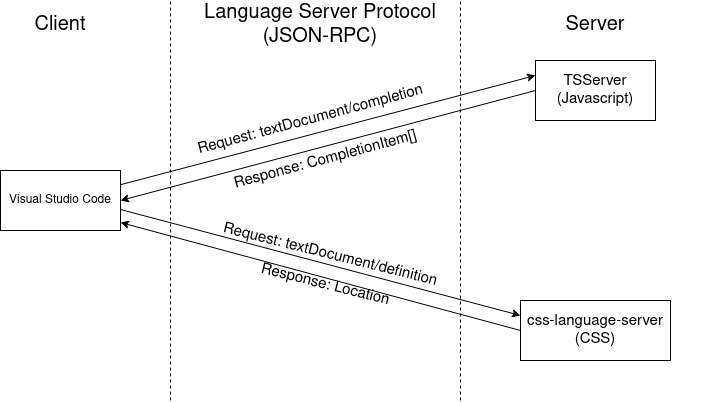
\includegraphics[width=\textwidth]{images/lspcommunication.png}
	\caption{Example client-server interaction using LSP}
	\label{fig:lspcommunication}
\end{figure}

\section{Preliminary algorithms and data structures}
\label{prelimalgos}

The following algorithms and data structures will be useful insight in following chapters to
define the detection algorithm

\subsubsection{Incremental-parsing}

While writing code, programmers usually only edit small regions of code at a time. One
``edit'' will therefore only affect small parts of the internal representations of the
code which most tools use to perform analysis. Reusing parts of this representation would
therefore be faster and allow programming tools to scale better. 

In our detection algorithm we will need to be able to parse our source code into an AST
representation in order to select specific syntactic regions and extract the tokens.
Therefore, we need a parsing algorithm, and when source code is edited we need an
incremental parsing algorithm to more efficiently parse the source code when only a
small region has been changed.

Incremental parsing is the process of reparsing only parts of a syntax tree whenever an
edit is performed. The motivation behind incremental parsing is to have a readily
available syntax tree after every edit, while doing as little computing as possible to
maintain it.

\verb|Tree-sitter| is a parser generator tool which specializes in incremental parsing. It
supports incremental parsing, error recovery and querying for specific nodes and
subtrees~\cite{treesitter}. These features combined allow Tree-sitter to become a powerful
tool for editing and has been used for IDE features such as syntax-highlighting,
refactoring and code navigation.

The incremental reparsing in Tree-sitter is performed using Wagner's
algorithm~\cite{PracticalAlgorithmsForIncremental}.

\Todo{Explain Wagner's algorithm with figure and example}

\subsubsection{Suffix trees}

A classic algorithm~\cite{Zibran_real_time_search, GodeIncrementalCloneDetection} for code
clone detection traverses a suffix-tree in order to find maximal repeats in all suffixes
of the input string T.

The suffix tree of a string $T$ is a compressed trie where all the suffixes of $T$ have been
inserted. The tree is compressed by combining consecutive nodes in a row which has
only one child into a single node. A common usage of a suffix tree is to determine whether
or not a suffix exists in $T$, and where in $T$ the suffix starts.

Figure \ref{fig:suffixtree} shows the suffix-tree for $T=\text{BANANA\$}$. In order to
determine where the suffix $\text{ANANA\$}$ exists in $T$, one can start from the root,
and traverse the tree, choosing the child node which correspond to the next character of
the suffix which has not been ``matched'' yet.

$$
\text{root} \xrightarrow{A} \text{node} \xrightarrow{\text{NA}} node \xrightarrow{\text{NA\$}} 1
$$

Following this path, we see that the suffix $\text{ANANA\$}$ exists in $T$ at index $1$.

Suffix trees can be constructed in linear time with Ukkonen's algorithm which builds a
larger and larger suffix tree by inserting characters one by one and utilizing some tricks
to avoid inserting suffixes before it needs to, lowering the complexity~\cite{Ukkonen}.

This data structure also facilitates solving the maximal repeat problem. A repeat in a
string T is a substring that occurs at least twice in T. A maximal repeat in T is a repeat
which is not a substring of another repeat in T, meaning that the maximal repeat cannot be
extended in any direction to form a bigger repeat. The problem of finding all maximal
repeats can be solved with a suffix tree using the following theorem:

\begin{theorem}[Repeats in suffix tree]

    Every internal node (except for the root) in a suffix tree corresponds to a substring
    which is repeated at least twice in T. The substring is found by concatenating the
    strings found on the path from the root of tree to the internal node.

\end{theorem}

This theorem is explained by the fact that any internal node has at least two children, and a
node having two children means that two suffixes share the same prefix up to that point.
An algorithm which finds the maximal repeats would find the internal nodes which
represents the longest strings. 

The classic algorithm~\cite{Zibran_real_time_search, GodeIncrementalCloneDetection} in
terms of finding duplication in a string (such as source code) using suffix trees would
find all repeats of length $k$, where $k$ is the threshold for how long a clone needs to
be. This can be found by traversing the suffix tree and looking at all internal nodes
which represent a string of length $\geq k$. Every internal node which represents a string
which is $\geq k$ would correspond to a substring of the source code which occurs at least
twice. Finding where the duplication occurs can be done by finding all the leaves of the
subtree rooted in the internal node, which each hold the position where the suffix starts in
T. Since a substring can have multiple repeats of different lengths longer than $k$,
different strategies can be used to select which substrings are selected or not, such as
filtering out repeats which are not maximal or repeats which contain or overlap each other.

In figure \ref{fig:suffixtree}, there are three repeats, ANA, A and NA. The only maximal
repeat would be ANA, since A and NA are not maximal.


\begin{figure}
	\begin{center}
		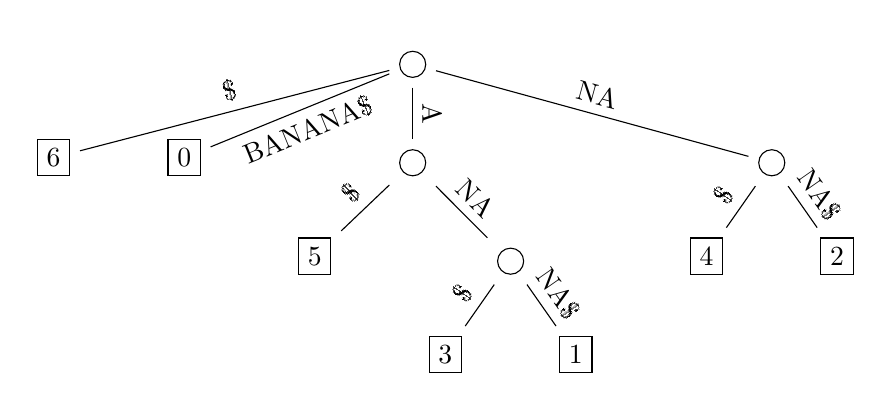
\begin{tikzpicture}[every tree node,
				level distance=1.25cm,sibling distance=1cm,
				edge from parent path={(\tikzparentnode) -- (\tikzchildnode)}]
			\Tree
			[.\addcircle{}
                \edge node[midway, above, sloped] {\$};
                [.\addsquare{6} ]
                \edge node[midway, below, sloped] {BANANA\$};
                [.\addsquare{0} ]
                \edge node[midway, above, sloped] {A};
                [.\addcircle{}
                    \edge node[midway, above, sloped] {\$};
                    [.\addsquare{5} ]
                    \edge node[midway, above, sloped] {NA};
                    [.\addcircle{}
                        \edge node[midway, above, sloped] {\$};
                        [.\addsquare{3} ]
                        \edge node[midway, above, sloped] {NA\$};
                        [.\addsquare{1} ]
                    ]
                ]
                \edge node[midway, above, sloped] {NA};
                [.\addcircle{}
                    \edge node[midway, above, sloped] {\$};
                    [.\addsquare{4} ]
                    \edge node[midway, above, sloped] {NA\$};
                    [.\addsquare{2} ]
			    ]
			]
		\end{tikzpicture}
		\caption{Suffix tree for $T=\text{BANANA\$}$}
        \label{fig:suffixtree}
	\end{center}
\end{figure}

\subsubsection{Suffix arrays}

The suffix array (SA) of a string T contains a lexicographical sorting of all suffixes in
T. The suffix array does not contain the actual suffixes, but it contains integers
pointing to the index where the suffix starts in T. Conversely, the inverse suffix array
(ISA) contains integers describing which rank the suffix at a given position has. The rank
of a suffix is its lexicographical ordering in $T$. ISA is therefore the inverse array
of SA, such that if $\text{SA}[i] = n$, then $\text{ISA}[n] = i$.

\begin{definition}[Suffix array] 
    Let T be a text of length N.
    The suffix array \texttt{SA} of T is an array of length N where $\text{SA}[i] = n$ if the
    suffix at $T[n..N-1]$ is the ith lexicographically smallest suffix in T.
\end{definition}

\begin{definition}[Inverse suffix array] 
    Let T be a text of length N.
    The inverse suffix array ISA of T is an array of length N where $ISA[i] = n$ if the
    suffix at $T[i..N-1]$ is the nth smallest suffix in T lexicographically.
\end{definition}

The Longest-common prefix (LCP) array describes how many common characters there are in a
prefix between two suffixes which are next to each other in the suffix array. Since the
suffix array represents suffixes in a sorted order, the prefix length between adjacent
suffixes in SA will be the longest possible common prefix for each suffix. These are the
values in the LCP array.

\begin{definition}[LCP array]
    Let T be a text of length N and SA be the suffix array of T.
    The LCP array of T is an array of length N where $\text{LCP[i] = n}$ if the suffix
    $\text{T[SA[i]..N]}$ and $\text{T[SA[i-1]..N]}$ has a maximal common prefix of length
    $\text{n}$. $\text{LCP[0]}$ is undefined or {0}.
\end{definition}

For example, in table \ref{table:BANANA}, the LCP value at position 3 contains the number
of characters in the longest-common prefix of suffixes starting at position 1 (ANANA\$)
and position 3 (ANA\$). These suffixes have 3 common characters in their prefix, therefore
the LCP value at position 3 is 3.

\begin{table}
	\begin{center}
        \subfloat[Suffixes]{
		\begin{tabular}{c | l }
			Index & Suffix   \\
			\hline
			0     & BANANA\$ \\
			1     & ANANA\$  \\
			2     & NANA\$   \\
			3     & ANA\$    \\
			4     & NA\$     \\
			5     & A\$      \\
			6     & \$       \\
    \end{tabular}}
		\hspace{1cm}
        \subfloat[Sorted suffixes]{\begin{tabular}{c | l}
			Index & Suffix   \\
			\hline
			6     & \$       \\
			5     & A\$      \\
			3     & ANA\$    \\
			1     & ANANA\$  \\
			0     & BANANA\$ \\
			4     & NA\$     \\
			2     & NANA\$   \\
    \end{tabular}}
		\hspace{1cm}
        \subfloat[SA, ISA and LCP]{\begin{tabular}{c | c | c | c}
                Index & SA & ISA & LCP \\
				\hline
                0     & 6  & 4   & 0\\
                1     & 5  & 3   & 0\\
                2     & 3  & 6   & 1\\
                3     & 1  & 2   & 3\\
                4     & 0  & 5   & 0\\
                5     & 4  & 1   & 0\\
                6     & 2  & 0   & 2\\
        \end{tabular}}
        \caption{$T=\text{BANANA\$}$}
        \label{table:BANANA}
	\end{center}
\end{table}


Suffix arrays can be constructed in linear time in terms of the length of T. Many suffix
array construction algorithms (SACA) have been discovered in the last
decade~\cite{SuffixArrayConstruction}, many of which run in linear-time. An algorithm which
has been shown to be very efficient in practice is Nong and Chan's algorithm based on
recursive suffix sorting of smaller strings~\cite{LinearTimeSuffixArraySAIS}. 

The enhanced (extended) suffix array is the suffix array and the additional LCP array,
which has been shown to be as powerful as a suffix tree, in terms of what can be computed
with it with the same time complexity, but uses a smaller amount of
memory~\cite{ReplaceSuffixTreeWithEnchancedSuffixArray}.

 \subsubsection{Dynamic bitsets}

A bitset is an array of bits, each bit representing either the value true or false. A bit
with the value of 1 is usually referred to as a set bit, and a value of 0 is referred to
as an unset or cleared bit. Bitsets have at least operations for setting the value at a
position, and looking up the value at a position. Bitsets are useful for many problems,
especially as a ``succinct data structure''. A succinct data structure is a data structure
which attempts to use an amount of memory close to the theoretic lower bound, while still
allowing effective queries on it. For example for a string of length $n$, we could store
up to $O(n \log_{}\sigma)$ bits before the bit vector exceeds the size of the string
itself, where $\sigma$ is the size of the string's alphabet.

The most well known query to do on bitsets is the rank/select queries.

\begin{definition}[Rank query on bitset]

    A rank query $rank_1(i)$ on a bitset B, computes the number of set bits
    up to, but not including position $i$. Conversely, $rank_0(B)$ returns the number of
    unset bits up to $i$.

\end{definition}
\begin{definition}[Select query on bitset]
    
    A select query $select_1(i)$ on a bitset B, computes the position of the ith
    set bit in B. Conversely, $select_0(i)$ returns the position of the ith unset bit in
    B.

\end{definition}

Jacobson's rank can calculate rank and select on static bitsets in $O(1)$ time by
pre-calculating all answers in a space efficient table~\cite{JacobsonsRank}.

\begin{definition}[Dynamic bitset]

    A dynamic bitset is a bitset which in addition to other operations allow inserting and
    deleting bits (indel operations).

    An insert operation $insert(i, v)$ on a bitset B inserts the value v at position i in
    B, pushing all values at position $\geq i$ one position up.

    A delete operation $delete(i)$ on a bitset B removes the value at position i in B, pushing all
    values at position $> i$ one position down.

\end{definition}

The standard implementation of a dynamic bitset would implement the whole bitset as a
single array of bytes $B$, which allows for accessing values in $O(1)$ time, but inserting
and deleting takes $O(n)$ time, where $n$ is the number of bits in $B$.

One way to speed up the indel operations would be to represent the bitset as a balanced
tree containing multiple smaller bitsets. To represent a bitset of $n$ bits, we can divide
the bits into smaller bitsets, such that $O(\frac{n}{\log(n)})$ bitsets each contains
$O(log(n))$ bits. Since the bitsets are now of size $O(log(n))$, inserting and deleting
takes only $O(log(n))$ time. The bitsets reside at the leaves of our balanced tree, and
internal nodes contain only two integers, storing the number of bits in the left subtree
($N$), and the number of set bits in the left subtree ($S$). To access, insert or delete
on index $i$, the tree is traversed to find the correct bitset where the ith bit is
located, where the operation is done at that position. Finding the correct bitset and
position is done by utilizing $N$ and $S$ in each node which is traversed. All operations
now run in $O(\log(n))$ time, since traversing the tree to the correct bitset takes
$O(\log(\frac{n}{\log(n)}))$ and performing the operation takes $O(\log(n))$ time. Keeping
the bitset balanced is done by splitting a leaf-node bitset to two nodes when the
leaf-node bitset has reached a certain size (such as $2 \times \log(n)$) and rebalancing
the tree after the split. Similarly, when considering deletions, two leaf-node bitsets can
be merged to their parent node when their combined number of bits has decreased to
$\log(n)$.


Figure \ref{fig:DynamicBitset} shows how a dynamic bitset tree is structured, and Algorithm
\ref{alg:dynbitaccess} shows how to access a value in the tree. Traversing the
tree to calculate rank and select queries can be done similarly by summing set
bits in left-subtrees (rank) or selecting which subtree to descend based on the number of
set bits (select).

\begin{figure}[t]
	\begin{center}
		\begin{tikzpicture}[every tree node,
				level distance=2cm,sibling distance=2cm,
				edge from parent path={(\tikzparentnode) -- (\tikzchildnode)}]
			\Tree
            [.\node[left, circle, draw, align=left, label={[align=left] above: $N = 8$\\$S = 3$}]{};
                \edge node[midway, above, sloped] {};
                [.\node[left, circle, draw, align=left, label={[align=left] above left:$N = 4$\\$S = 2$}]{};
                    \edge node[midway, above, sloped] {};
                    [.\addsquare{0101} ]
                    \edge node[midway, above, sloped] {};
                    [.\addsquare{0001} ]
                ]
                \edge node[midway, above, sloped] {};
                [.\node[left, circle, draw, align=right, label={[align=right] above right:$N = 4$\\$S = 1$}]{};
                    \edge node[midway, above, sloped] {};
                    [.\addsquare{0100} ]
                    \edge node[midway, above, sloped] {};
                    [.\addsquare{0000} ]
                ]
            ]
		\end{tikzpicture}
		\caption{Dynamic bitset}
        \label{fig:DynamicBitset}
	\end{center}
\end{figure}

\begin{algorithm}[htp]
  \SetAlgoLined\DontPrintSemicolon
    \algo{\access{node, i}}{
        \If{{\isLeaf{node}}}{
            \Return $\ArrayAccess{\Access{\Var{node}}{\Var{bitset}}}{\Var{i}}$
        }

        \If{$\Access{\Var{node}}{\Var{N}} \leq \Var{i}$}{
            \Return \access{$\Access{\Var{node}}{\Var{left}}, \Var{i}$}
        }

        \Return \access{$\Access{\Var{node}}{\Var{right}}, \Var{i} - \Access{\Var{node}}{\Var{N}}$}
    }

  \vspace{0.5cm}
  \caption{Accessing a value in a dynamic bitset}
  \label{alg:dynbitaccess}
\end{algorithm}

\subsubsection{Wavelet tree and wavelet matrix}

We can extend the notion of rank and select queries to strings as well. 

\begin{definition}[Rank query on string]

    A rank query $rank_c(i)$ on a string $S$ computes the number of occurrences of $c$
    in $S$ up to, but not including position $i$.

\end{definition}
\begin{definition}[Select query on string]

    A select query $select_a(i)$ on a string $S$, computes the position of the ith
    occurrence of $a$ in $S$. 

\end{definition}

The classic data structure to efficiently compute $rank$ and $select$ queries on strings
is the \textbf{wavelet tree}~\cite{WaveletTree}. The data structure is a binary tree where every
node consists of a bitset, and each level of the tree consists of the bits of a single
position in each character of the string. Each bitset in the wavelet tree can for example
be implemented as a dynamic bitset to allow indel operations on a wavelet tree.

\begin{figure}[t]
	\begin{center}
		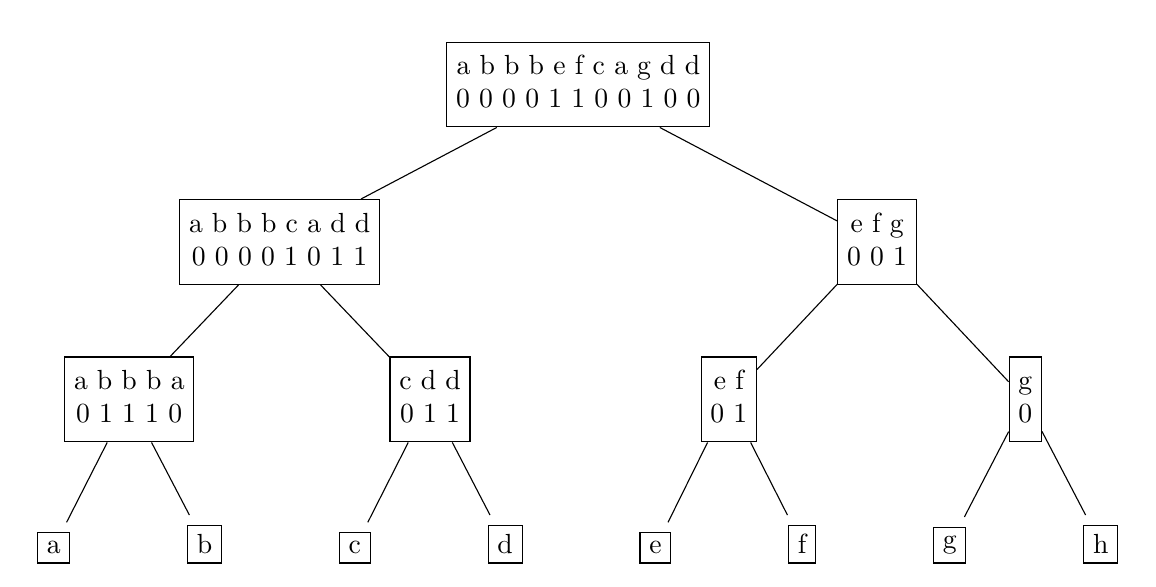
\begin{tikzpicture}[every tree node,
				level distance=2cm,sibling distance=1.25cm,
				edge from parent path={(\tikzparentnode) -- (\tikzchildnode)}]
			\Tree
            [.\node[draw,
                align=center]{\tabbedCenterstack{a b b b e f c a g d d\\0 0 0 0 1 1 0 0 1 0 0}};
                \edge node[midway, above, sloped] {};
                [.\node[draw, align=center]{\tabbedCenterstack{a b b b c a d d\\0 0 0 0 1 0 1 1}};
                    \edge node[midway, above, sloped] {};
                    [.\node[draw, align=center]{\tabbedCenterstack{a b b b a\\0 1 1 1 0}};
                        \edge node[midway, above, sloped] {};
                        [.\addsquare{a} ]
                        \edge node[midway, above, sloped] {};
                        [.\addsquare{b} ]
                    ]
                    \edge node[midway, above, sloped] {};
                    [.\node[draw, align=center]{\tabbedCenterstack{c d d\\0 1 1}};
                        \edge node[midway, above, sloped] {};
                        [.\addsquare{c} ]
                        \edge node[midway, above, sloped] {};
                        [.\addsquare{d} ]
                    ]
                ]
                \edge node[midway, above, sloped] {};
                [.\node[draw, align=center]{\tabbedCenterstack{e f g\\0 0 1}};
                    \edge node[midway, above, sloped] {};
                    [.\node[draw, align=center]{\tabbedCenterstack{e f\\0 1}};
                        \edge node[midway, above, sloped] {};
                        [.\addsquare{e} ]
                        \edge node[midway, above, sloped] {};
                        [.\addsquare{f} ]
                    ]
                    \edge node[midway, above, sloped] {};
                    [.\node[draw, align=center]{\tabbedCenterstack{g\\0}};
                        \edge node[midway, above, sloped] {};
                        [.\addsquare{g} ]
                        \edge node[midway, above, sloped] {};
                        [.\addsquare{h} ]
                    ]
                ]
            ]
		\end{tikzpicture}
		\caption{Wavelet tree for S = abbbefcagdd}
        \label{fig:wavelettree}
	\end{center}
\end{figure}


\begin{table}[t!]
	\begin{center}
		\begin{tabular}{c}
            \begin{tabular}{c c c c c c c c c c c c}
                a & b & b & b & e & f & c & a & g & d & d \\
                \hline
            \end{tabular} \\
            \begin{tabular}{c c c c c c c c c c c c}
                0 & 0 & 0 & 0 & 1 & 1 & 0 & 0 & 1 & 0 & 0
            \end{tabular} \\
            \begin{tabular}{c c c c c c c c|c c c}
                0 & 1 & 1 & 1 & 1 & 0 & 1 & 1 & 0 & 1 & 1
            \end{tabular} \\
            \begin{tabular}{c c c c c|c c c|c c|c}
                0 & 1 & 1 & 1 & 0 & 0 & 1 & 1 & 0 & 1 & 0
            \end{tabular} \\
		\end{tabular}
		\caption{Levelwise wavelet tree}
		\label{table:levelwisewavelettree}
	\end{center}
\end{table}




Figure \ref{fig:wavelettree} shows the wavelet tree for the string \verb|abbbefcagdd|. The
wavelet tree can perform $access$, $rank$ and $select$ queries by traversing the tree from
root to leaf. 

$access(i)$ gives the bitstring of the character at a position $i$ by first accessing
position $i$ in the root bitset, if the bit is a $0$, we traverse to the left, if it is a
$1$ we traverse to the right. Before traversing to a child, we compute $rank_0(i)$ or
$rank_1(i)$, depending on what bit is at position $i$, the resulting rank is the next
position to consider in the subtree. This is done recursively until a leaf-node is found,
and the bits which were examined at each node is the bitstring of the character at
position $i$.

$rank_c(i)$ traverses the tree similarly to $access(i)$, but we use the bits of $c$ to
guide us to the correct subtree. When a leaf-node is reached, the value of $i$ is
returned, since when a leaf is reached, $i$ will be pointing to the correct rank in the
fictitious bitset of only $a$ characters

The wavelet tree can be traversed in $O(\log \sigma)$ time where $\sigma$ is the size of
the alphabet. However, the $access$, $rank$ and $select$ operations also depend on how
fast the bitsets can perform $access$, $rank$ and $select$ operations. If the bitsets are
implemented using for example Jacobson's rank~\cite{JacobsonsRank}, the bitsets have a
$O(1)$ $access$, $rank$ and $select$ time, but if we require dynamic bitsets for indel
operations, the time complexity drops to $O(\log n \log \sigma)$ because a bitset
operation which takes $O(\log n)$ time is required in each level of the tree.

The wavelet tree can also be implemented without pointers, known as a levelwise or
pointerless wavelet tree\cite{LevelwiseWaveletTree}. Table \ref{table:levelwisewavelettree}
shows the levelwise wavelet tree, which can be traversed level by level, but determining
which interval of the bitset the node you are in occupies requires two calls to $rank$.
The details of the levelwise wavelet trees are out of scope for this thesis, but leads us
into the next wavelet data structure.

The \textbf{wavelet matrix} is a relatively recent improvement on the wavelet tree, which
has been shown to be more efficient for $access$, $rank$ and $select$ queries, as well as
less memory intensive for larger alphabets~\cite{WaveletMatrix}. As the name suggests, the
wavelet matrix is a matrix of bitsets, instead of a tree of bitsets. Similarly to the
levelwise wavelet tree, for a string $S$ of size $n$, each level of the matrix consists of
a bitset of size $n$. The difference between a levelwise wavelet tree and a wavelet matrix
is that the assumption that the "children" of an interval $[x, y]$ needs to occupy exactly
$[x, y]$ is no longer true. We can instead simply put all $0$ bits to the left in the next
level, and all $1$ bits to the right. For each level we store an integer $z_l$, which
holds the number of zero bits in level $l$. 

For $access$ operations, we traverse each level similarly to a levelwise wavelet tree, but
instead of traversing a smaller and smaller interval in each level, we simply look at the
current bit at position $i$, if it is a zero, the bit to examine in the next level is
$rank_0(i)$, if the bit is a $1$, the bit to examine in the next level is $z_l +
rank_1(i)$. $rank_c(i)$ operation is carried out similarly, but we also keep track of a
preceding position to the final $i$, which we subtract from $i$, to count only the number
of proceeding number of $a$ characters. Table \ref{table:waveletmatrix} shows an example
wavelet matrix, and algorithm \ref{alg:waveletmatrixaccess} and
\ref{alg:waveletmatrixrank} shows how $access$ and $rank$ operations can be carried out
for a wavelet matrix.

\begin{table}[t]
	\begin{center}
		\begin{tabular}{c}
            \begin{tabular}{c c c c c c c c c c c c}
                a & b & b & b & e & f & c & a & g & d & d \\
                \hline
                0 & 0 & 0 & 0 & 1 & 1 & 0 & 0 & 1 & 0 & 0 \\
                0 & 0 & 0 & 0 & 1 & 0 & 1 & 1 & 0 & 0 & 1 \\
                0 & 1 & 1 & 1 & 0 & 0 & 1 & 0 & 1 & 1 & 0
            \end{tabular} \\
		\end{tabular}
		\caption{Wavelet matrix for S = abbbefcagdd}
		\label{table:waveletmatrix}
	\end{center}
\end{table}


\begin{figure}
\begin{minipage}{0.46\textwidth}
    \begin{algorithm}[H]
        \SetAlgoLined\DontPrintSemicolon
        \algo{\access{WM, i}}{
            $\Var{bits} \gets \textrm{empty\ list}$ \;
            $\Var{l} \gets 0$ \;
            \While{$\Var{l} < \Len{$\Var{WM}$}$}{
                \Add{$\Var{bits}, \access{$\ArrayAccess{\Var{WM}}{\Var{l}}, \Var{i}$}$} \;
                \uIf{$\access{$\ArrayAccess{\Var{WM}}{\Var{l}}, \Var{i}$} = 1$}{
                    $\Var{i} \gets z_l + \RankOne{$\ArrayAccess{\Var{WM}}{\Var{l}}, \Var{i}$}$ \;
                }
                \Else{
                    $\Var{i} \gets \RankZero{$\ArrayAccess{\Var{WM}}{\Var{l}}, \Var{i}$}$ \;
                }
                $\Var{l} \gets \Var{l} + 1$
            }
            \Return $\Var{bits}$ \;
        }
        \caption{Wavelet matrix access}
        \label{alg:waveletmatrixaccess}
    \end{algorithm}
\end{minipage}
\begin{minipage}{0.46\textwidth}
    \begin{algorithm}[H]
        \SetAlgoLined\DontPrintSemicolon
        \algo{\RankC{WM, i}}{
            $\Var{l} \gets 0$ \;
            $\Var{p} \gets 0$ \;
            \While{$\Var{l} < \Len{$\Var{WM}$}$}{
                \uIf{$\access{$\ArrayAccess{\Var{WM}}{\Var{l}}, \Var{i}$} = 1$}{
                    $\Var{i} \gets z_l + \RankOne{$\ArrayAccess{\Var{WM}}{\Var{l}}, \Var{i}$}$ \;
                    $\Var{p} \gets z_l + \RankOne{$\ArrayAccess{\Var{WM}}{\Var{l}}, \Var{p}$}$ \;
                }
                \Else{
                    $\Var{i} \gets \RankZero{$\ArrayAccess{\Var{WM}}{\Var{l}}, \Var{i}$}$ \;
                    $\Var{p} \gets \RankZero{$\ArrayAccess{\Var{WM}}{\Var{l}}, \Var{p}$}$ \;
                }
                $\Var{l} \gets \Var{l} + 1$
            }
            \Return $\Var{i} - \Var{p}$ \;
        }
        \caption{Wavelet matrix rank}
        \label{alg:waveletmatrixrank}
    \end{algorithm}
\end{minipage}
\end{figure}

The wavelet matrix is constructed level by level. In level $i$, the bit at position $i$ in
each character is inserted. Before constructing the next level, each character is sorted
by the current bit, so that all the characters with $0$ bits at position $i$ occupies the
left side of level $i + 1$, and vice versa for $1$ bits.

\subsubsection{Burrows-Wheeler transform}

\begin{table}[t]
	\begin{center}
        \subfloat[Cyclic shifts]{
		\begin{tabular}{c | l }
			Index & Cyclic-shift   \\
			\hline
			0     & BANANA\$ \\
			1     & ANANA\$B \\
			2     & NANA\$BA \\
			3     & ANA\$BAN \\
			4     & NA\$BANA \\
			5     & A\$BANAN \\
			6     & \$BANANA \\
    \end{tabular}}
		\hspace{0.5cm}
        \subfloat[Sorted cyclic shifts and BWT]{\begin{tabular}{c | l}
			Index & Cyclic-shift   \\
			\hline
            6     & \$BANAN\textbf{A} \\
            5     & A\$BANA\textbf{N} \\
			3     & ANA\$BA\textbf{N} \\
			1     & ANANA\$\textbf{B} \\
			0     & BANANA\textbf{\$} \\
			4     & NA\$BAN\textbf{A} \\
			2     & NANA\$B\textbf{A} \\
    \end{tabular}}
		\hspace{0.5cm}
        \subfloat[LF function]{\begin{tabular}{c | l}
			L & F   \\
			\hline
            0     & $Rank_A(0) + C[A] = 0 + 1 = 1$\\
            1     & $Rank_N(1) + C[N] = 0 + 5 = 5$ \\
			2     & $Rank_N(2) + C[N] = 1 + 5 = 6$ \\
			3     & $Rank_B(3) + C[B] = 0 + 4 = 4$ \\
            4     & $Rank_{\$}(4) + C[\$] = 0 + 0 = 0$ \\
			5     & $Rank_A(5) + C[A] = 1 + 1 = 2$ \\
			6     & $Rank_A(6) + C[A] = 2 + 1 = 3$ \\
    \end{tabular}}
    \caption{S = BANANA\$, BWT = ANNB\$AA}
    \label{table:bwt}
	\end{center}
\end{table}

The Burrows-Wheeler transform (BWT) is a transform on strings, often performed on strings
to improve compression~\cite{BWT}. The transform is computed by sorting all
``cyclic-shifts'' of the string lexicographically and extracting a new string from the
last column of the cyclic-shift'' matrix. \$ is added to the string as a unique
terminating character, this makes some of the algorithms on the BWT simpler. \$ is always
the smallest character lexicographically. Table \ref{table:bwt} shows the BWT for the
string S = BANANA\$.

\begin{definition}{Cyclic-shift}

    The cyclic-shift of order $i$ for a string $S$ is the cyclic-shift of $S$ such that
    all characters in $S$ are rotated $i$ characters to the left. The cyclic-shift of
    order $i$ is denoted $CS_i$

\end{definition}

\begin{definition}{Burrows-Wheeler transform}

    The Burrows-Wheeler transform of a string $S$ is a transformation on $S$ where the
    cyclic-shifts of $S$ are sorted, and the final character in each shift is concatenated.

\end{definition}

There is a direct correlation between the suffix array of S and the BWT of S. Table
\ref{table:bwt} also shows that the indices of the sorted cyclic-shifts correspond to
exactly the SA of S. This coincides because when sorting cyclic-shifts, everything that
occurs after the \$ of the cyclic-shift will not affect its lexicographical ordering. This
is because no cyclic-shift will have a \$ in the same position, so comparing two cyclic
shifts lexicographically will always terminate whenever a \$ is found. This means that the
ordering of cyclic shifts is essentially the same as sorting all suffixes of S. Algorithm
\ref{alg:bwt} shows how the BWT of S can be calculated directly from the SA of S in linear
time. Since this is a one to one correlation between the SA and BWT, dynamic updates to a BWT
would correspond to similar dynamic updates in the SA (and ISA). This will be useful in
the following implementation chapter for the dynamic code clone detection algorithm.

\begin{algorithm}[htp]
  \SetAlgoLined\DontPrintSemicolon
    \algo{\ComputeBWT{S, SA}}{
        $\Var{n} \gets \Access{S}{len}$

        $BWT \gets \mathrm{string\ of\ length\ } n$

        \For{$i \From 0 \To \Var{n}$}{

            $\Var{pos} \gets (\SA{\Var{i}} - 1)\ \%\ n$

            $\BWT{i} = \ArrayAccess{\Var{S}}{pos}$
        }

        \Return BWT
    }

  \vspace{0.5cm}
  \caption{Calculating the BWT of a string T from its suffix array}
  \label{alg:bwt}
\end{algorithm}


An essential property of the BWT is that the transformation is reversible. By examining
the BWT of a string T, we see that the BWT is a permutation of T. We will also see that
there is a correlation between the characters in the first column of the cyclic-shift
matrix and the last column (the BWT).

T can be calculated from the BWT as long as there is a unique terminating character (\$),
or the position of the final character is stored. T is computed backwards by starting at
the final character ($T[n - 1]$) and then finding the cyclic-shift where that character
occurs in the first column (the previous cyclic-shift). The character in the last column
of that cyclic-shift is $T[n - 2]$. If there are multiple of the same character, the nth
occurrence of a certain symbol in the last column will map to the nth occurrence of the
same symbol in the first column. This process is repeated until we finish the cycle,
returning to the final character in the last column. Essentially, this process consists of
traversing cyclic-shifts backwards and looking at the final character, which will give us
T, since the final character of the cyclic-shift is continually shifting one position.

We can use the fact that the first column consists of the letters of T in sorted order to
determine the previous cyclic-shift with only the last column. We can calculate the
previous cyclic-shift from only the last column by determining how many characters are
lexicographically smaller than the current character, and also the rank of the current
character at this position. The sum of these two values is the location of the previous
cyclic-shift. This function is called the Last-to-first function (LF function).
Calculating the LF function can be done efficiently by using a rank/select data structure
such as a wavelet tree~\cite{WaveletTree} or wavelet matrix~\cite{WaveletMatrix} to
calculate the rank of all the characters in the BWT, and an array $C$ which contains the
number of occurrences of each letter in the BWT.

The LF function will also be useful in the detection algorithm when dynamically updating
the suffix array.


\chapter{Implementation: LSP server architecture}
\label{lspimplementation}

The following chapters will discuss how CCDetect-LSP is implemented, and especially
focuses on our novel algorithm based on dynamic extended suffix
arrays\footnote{CCDetect-LSP source code is available here:
\url{https://github.com/jakobkhansen/CCDetect-lsp}}. The current chapter will look at the
LSP integration and how source code is initially indexed, while the following two chapters
will discuss first how clones are initially detected and then how this analysis in
incrementally updated as source code changes.

CCDetect-LSP is integrated into IDEs via LSP. The tool starts up as an LSP server, which
an IDE client can connect to and send/receive messages from. The goal of the LSP
client-server interaction is to give users of the tool an overview of all clones as they
appear in source code, and allow them to navigate between matching clones. CCDetect-LSP is
implemented in Java with the LSP4J library which provides an abstraction layer on top of
the protocol which is easier to work with programmatically.

\begin{figure}[ht!]
	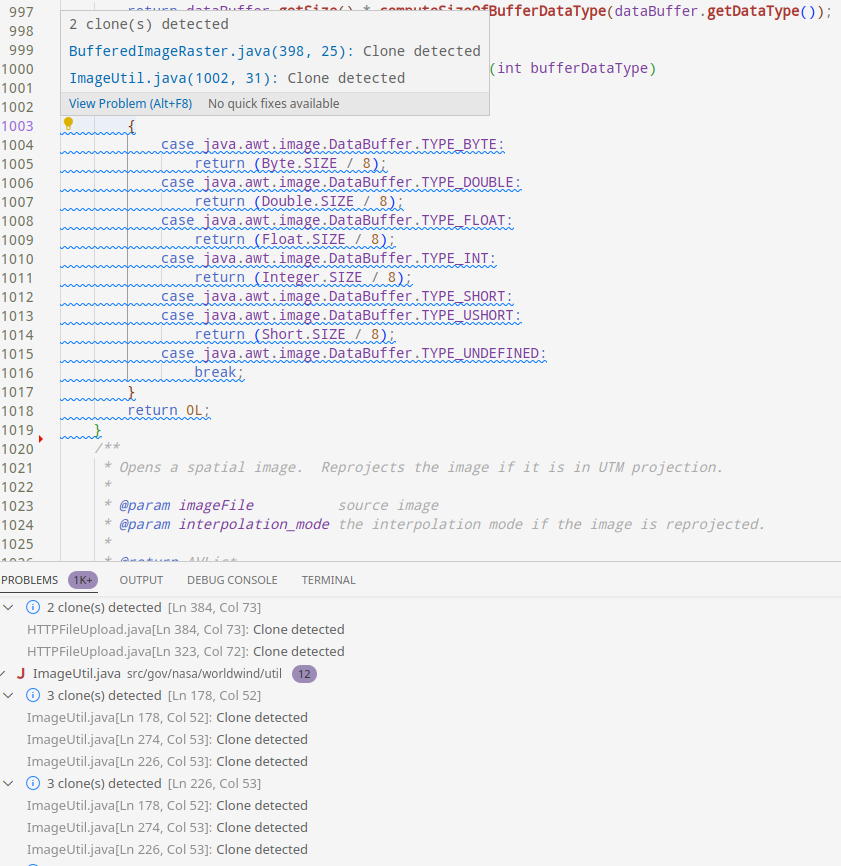
\includegraphics[width=\textwidth]{figures/vscodecodeclone.png}
	\caption{Code clones displayed in the VSCode IDE}
	\label{fig:vscodeclones}
\end{figure}

\begin{figure}[t]
	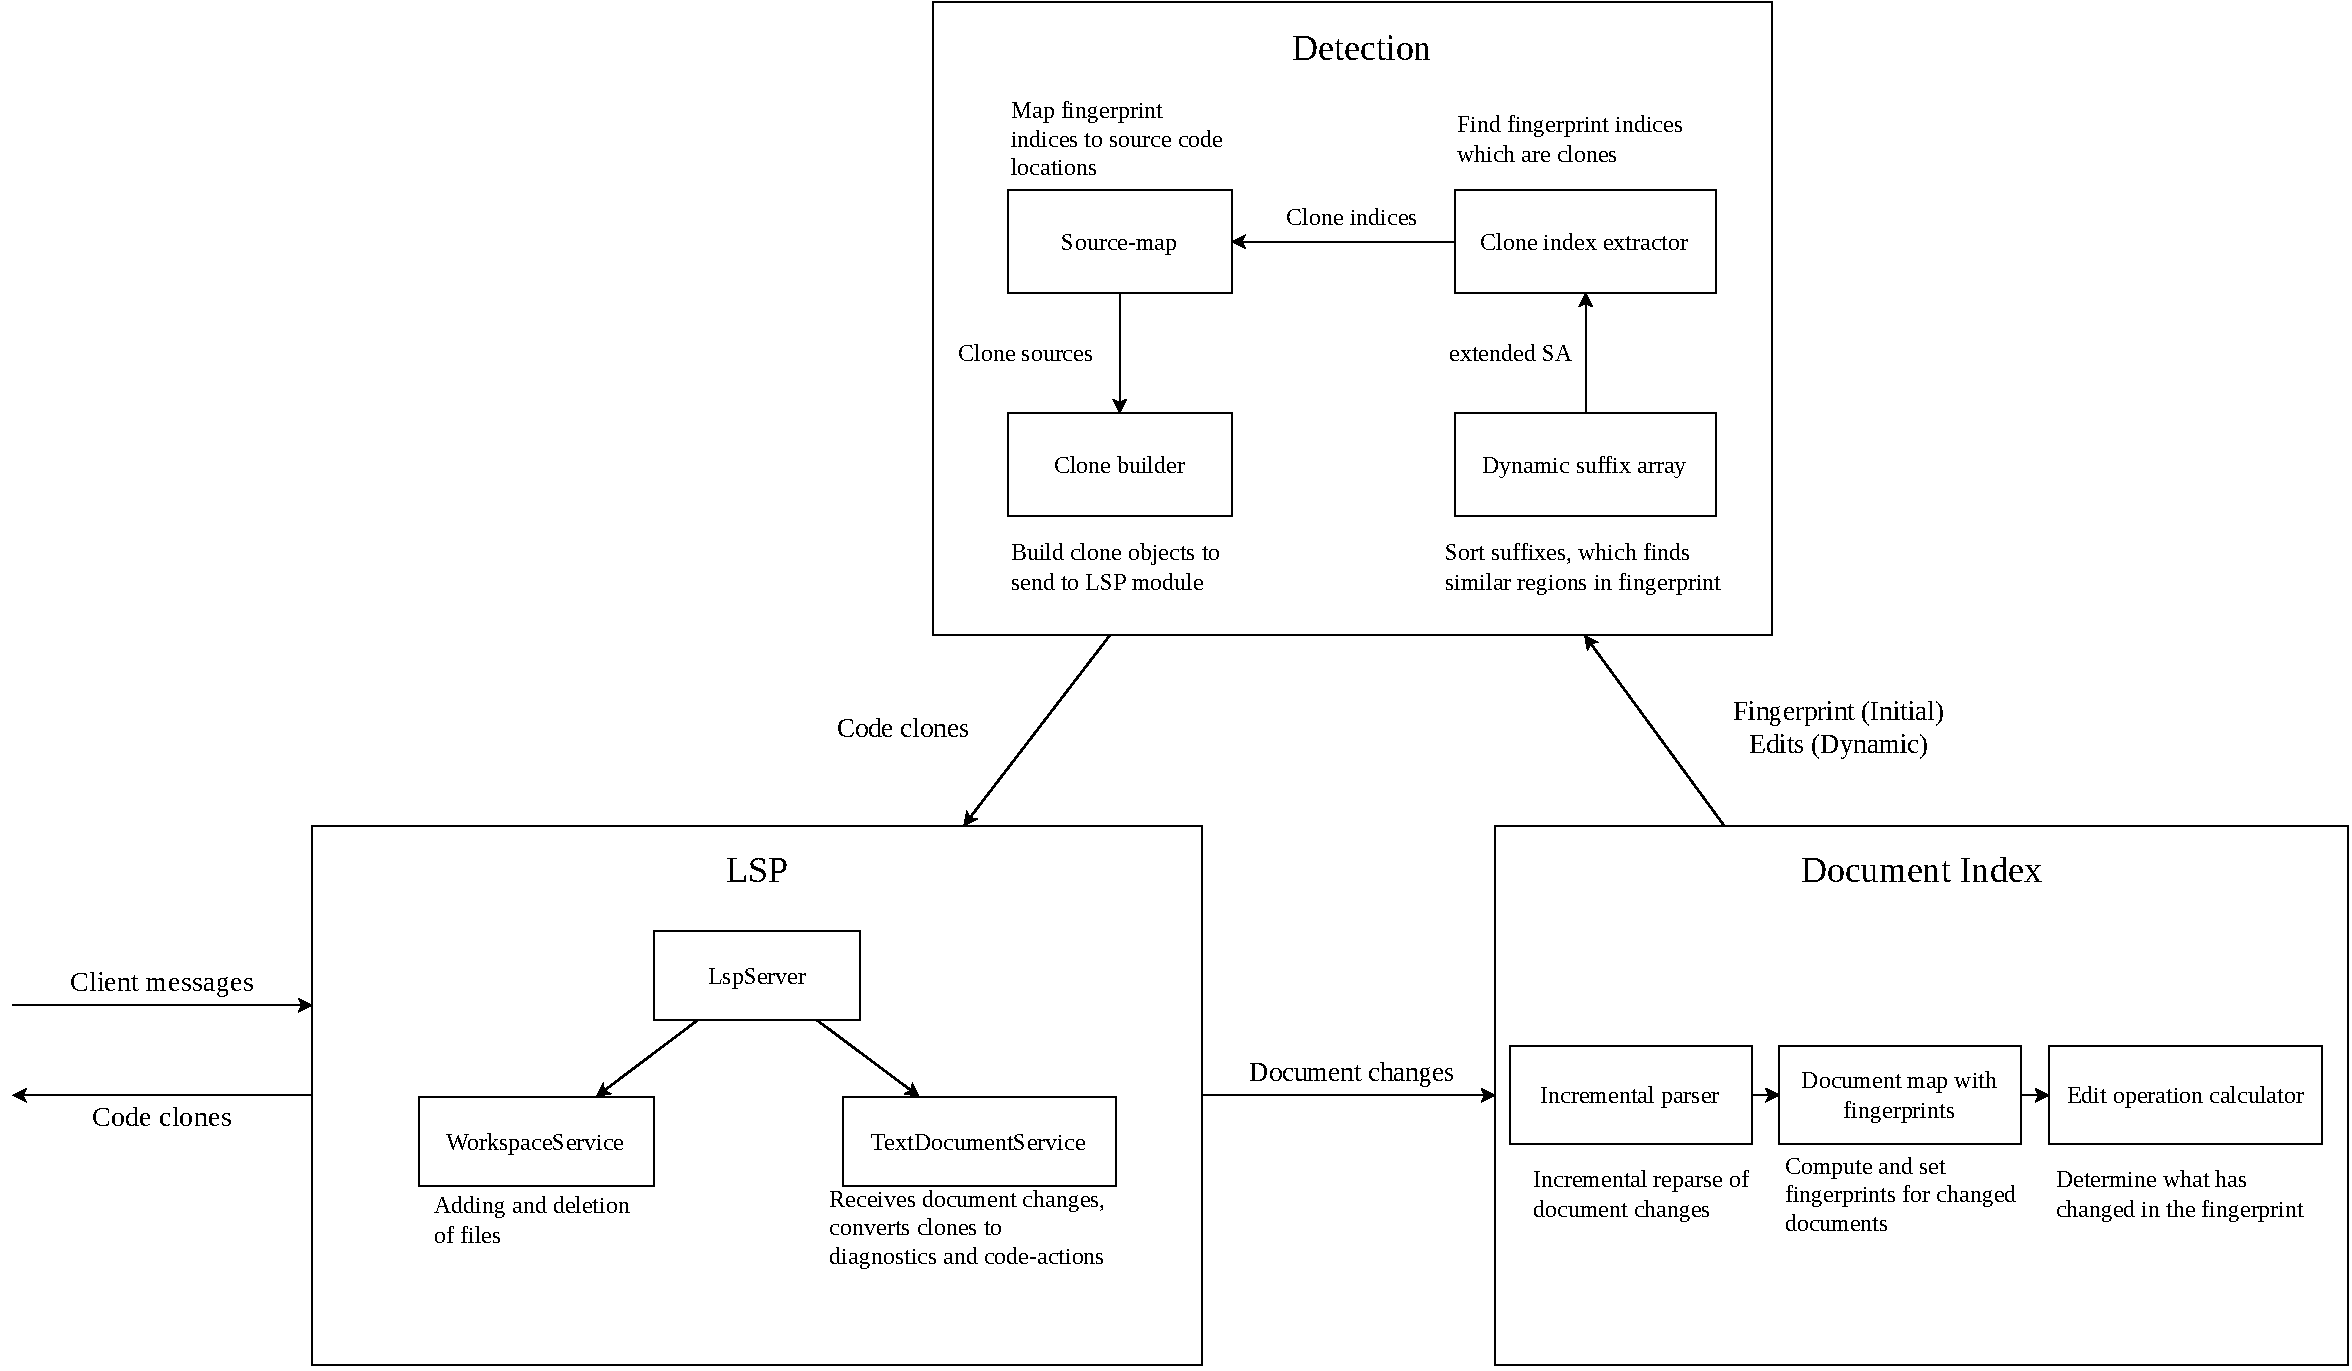
\includegraphics[width=\textwidth]{figures/architecture.drawio.pdf}
	\caption{Tool architecture}
	\label{fig:architecture}
\end{figure}


Figure \ref{fig:vscodeclones} shows how clones are displayed in the VSCode IDE. The image
shows a section of a file where a Java switch statement has been duplicated in two other
files. Code clones are displayed inline in the file as an ``Information'' diagnostic, and
when hovered over, the client shows the \verb|DiagnosticRelatedInformation| information of
the diagnostic where all the matching clones are displayed and can be clicked to navigate
to the corresponding match. For a client which may not implement the
\verb|DiagnosticRelatedInformation| message\footnote{Added to LSP in version 3.16,
released in 2020. In our experience, some IDEs do not implement this feature.}, invoking a
code-action to navigate to the matching clone is another option.

The following user-stories shows how interaction with the LSP server works.

\begin{itemize} 

    \item A programmer wants to see code clones for a file in their project, the
        programmer opens the file in their IDE and is shown diagnostics inline with the
        code wherever there are detected clones. The matching code clones are not
        necessarily in the same file.

	\item A programmer wants to see all code clones for the current project. The
	      programmer opens the IDEs diagnostic view and will see all code clones detected
	      as diagnostics there. The diagnostic will contain information like where the clone
	      exists, and where the matching clone(s) are.

    \item A programmer wants to jump to one of the matches of a code clone in their IDE.
        The programmer moves their cursor to the diagnostic and will see a list of the
        matching code clones. The programmer selects any of the code clones which will
        open the file and location of the selected code clone. Alternatively, a
        code-action can be invoked to navigate, if the client does not implement the
        \verb|DiagnosticRelatedInformation| interface.

      \item A programmer wants to refactor a set of clones by applying the
          ``extract-method'' refactoring (not implemented by CCDetect-LSP). The programmer
          performs the necessary refactorings, and will see that the refactored clones are
          no longer detected when the LSP server incrementally updates its analysis.

\end{itemize}


Figure \ref{fig:architecture} shows the architecture of the tool. The LSP module
communicates with the IDE and delegates the work of handling documents to the document
index. Detection of clones is delegated to the detection module. The LSP module receives a
list of clones from the detection module which is then converted to LSP diagnostics and
code-actions which is finally sent to the client.

\section{Document index}

Upon starting, the LSP server needs to index the project. This involves creating an index
and inserting all the relevant documents in the code base. A document contains the content
of a file along with extra information such as the file's URI and some information which
is useful for the later clone detection. We define the following record for our documents:

\begin{lstlisting}
    Document {
        String uri,
        String content,
        AST ast,

        // Location in fingerprint
        int start,
        int end

        // Used for incremental updates
        int[] fingerprint,
        boolean open,
        boolean changed,
    }
\end{lstlisting}

Each document in the index primarily consists of the contents, the URI and the AST of the
document in its current state. Storing the AST will be useful for the incremental
detection algorithm.

There are two things to consider when determining which files should be inserted into the
index. First, we are considering only files of a specific file type, since the tool does
not allow analysis of multiple programming languages at the same time. Therefore, the
index should contain for example only \verb|*.java| files if Java is the language to
analyze. Secondly, all files of that file type might not be relevant to consider in the
analysis. This could for example be generated code, which generally contains a lot of
duplication, but is not practical or necessary to consider as duplicate code, since this
is not code which the programmer interact with directly. Therefore, the default behavior
is to consider only files of the correct file type, which are checked into Git. The tool
supports adding all files in a folder, or all files checked into Git.

When a document is first indexed by the server, the file contents is read from the disk.
However, as soon as the programmer opens this file in their IDE, the source of truth for
the files content is no longer on the disk, as the programmer is changing the file
continuously before writing to the disk. The LSP protocol defines multiple JSON-RPC
messages which the client sends to the server in order for the server to keep track of
which files are opened, and the state of the content of opened files.

Upon opening a file, the client will send a \verb|textDocument/didOpen| message to the
server, which contains the URI for the opened file. The index will at this point set the
flag \verb|open| for the relevant document and stops reading its contents from disk.
Instead, updates to the file are obtained via the \verb|textDocument/didChange| message.
This message can provide either the entire content of the file each time the file changes,
or it can provide only the changes and the location of the change. Receiving only the
changes will be useful for this algorithm when the analysis incrementally reparses the
document.

\section{Displaying and interacting with clones}

When detection is finished and the list of clones is ready, the LSP module will convert
clones into diagnostics and code-actions which can be interacted with from the client. For
diagnostics, each clone object is converted into a diagnostic which has a range and some
information about the clone. The diagnostic displays an error in the client which also has
information for each matching clone. This is achieved this by attaching
\verb|DiagnosticRelatedInformation| to a diagnostic which is defined in the protocol. When
all the code clones have been converted to diagnostics, the server sends a
\verb|textDocument/publishDiagnostics| message which sends all the diagnostics to the
client in JSON-RPC format. For code-actions, the process is similar, for each clone pair,
we create a code-action which navigates from one to the other, using the
\verb|window/showDocument| message. These code-actions are similarly sent to the client
via the \verb|textDocument/codeAction| message, but this message is only invoked when the
client specifically requests code actions at a certain location.


\chapter{Implementation: Initial detection}
\label{initialdetection}

\begin{figure}[H]
    \begin{center}
        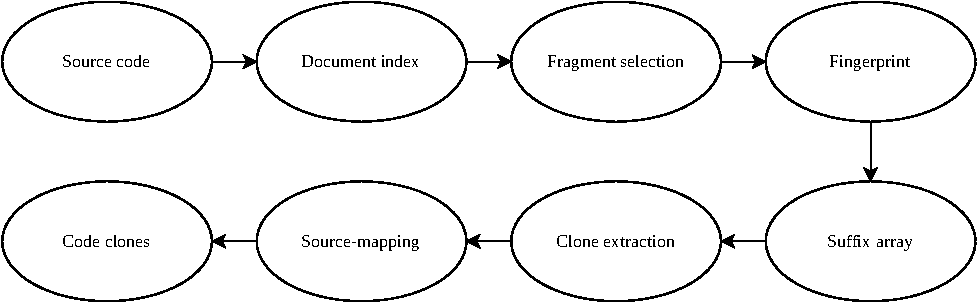
\includegraphics[width=0.8\textwidth]{figures/phases/phases_all.drawio.pdf}
    \end{center}
    \caption{Phases of the detection algorithm}
    \label{fig:allphases}
\end{figure}

This chapter discusses the detection module of CCDetect-LSP and how the initial detection
algorithm finds code clones. It consists of the detection algorithm which takes the
document index as input, and outputs a list of code clones. The initial input to the
algorithm will be the raw source code of each document in the index, in text format.
Figure \ref{fig:allphases} shows all the phases of the detection algorithm and in each
section a figure will be shown to illustrate which part of the pipeline is currently being
discussed. The previous chapter has already detailed the first two phases, how a document
index is built for each file of the source code.

The algorithm of CCDetect-LSP detects syntactical type-1 and allows configuration to
detect blind type-2 code clones as well. Clones are detected based on a token threshold,
which means clones are snippets of source-code which have at least $N$ equal tokens, where
$N$ is a configurable parameter. 

Without extra configuration, the clones detected are exactly equal (type-1), but allows
differences in for example white-space, and anything else which is not parsed into the
syntax-tree. Additionally, Tree-sitter grammars often mark some AST nodes such as comments
as ``extra'' nodes, which are ignored. There is also a configurable parameter to ignore
additional nodes. 

For type-2 detection, the client can configure which token types are allowed to have
different values, which makes blind type-2 clone detection possible.  

Finally, there are also two additional rules which govern which clones are included in the
list of reported clones.

\begin{itemize}
    \item Clones which are completely contained within another larger clone are excluded.
    \item Clones cannot extend past the end of a fragment.
\end{itemize}

In broad strokes, the algorithm first selects the relevant parts of source code to detect
code clones in (fragment selection), then transforms the selected fragments into a smaller
representation and normalizes the input for type-2 detection (fingerprinting). For the
matching, an extended suffix array for the fingerprint is constructed, where the LCP array
is used to find long matching instances of source code. Finally, clones are filtered and
aggregated into clone classes before they are source-mapped back to the original
source-code locations, which the LSP server can send to the IDE in the form of
diagnostics.

The decision to go with extended suffix arrays were based on the fact that extended suffix
arrays use less memory than the traditional suffix tree approach, which is important in an
IDE scenario. We also wanted to explore dynamic extended suffix arrays to determine if it
could be a better approach to clone detection in regard to performance as well, as we are
not aware of any related work which implements a dynamic extended suffix array and
compares its performance with a dynamic suffix tree for clone detection.

\section{Fragment selection}

\begin{figure}[H]
    \begin{center}
        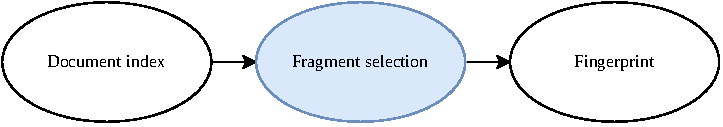
\includegraphics[width=0.8\textwidth]{figures/phases/phases_fragmentselection.drawio.pdf}
    \end{center}
\end{figure}

The first phase of the algorithm involves extracting the relevant fragments of source code
which should be considered for detection. A fragment, in this case is an instance of a
particular type of node in the AST. The tokens the node encompasses is in this phase
extracted and used in the subsequent phases. Note that in a concrete syntax tree, each
leaf-node encompasses a single token, which means that selecting a node and extracting its
tokens involves extracting all the leaf-nodes in the subtree of the selected
node\footnote{For type-2 detection we say that we consider certain token types. This is
actually AST leaf-node types, not tokens, but we will call them token types, as it is
essentially the same.}. Since the algorithm is language agnostic, it is not feasible to
have a single algorithm for fragment extraction or to define a separate fragment
extraction algorithm for every possible language. Therefore, a parser generator tool is
used, which can generate the code for parsing any programming language given a grammar. We
use Tree-sitter, a parser generator with incremental parsing capabilities, as well as a
query language for finding any type of node or subtree in the AST~\cite{treesitter}.
Tree-sitter queries are flexible queries to select specific nodes or subtrees. For
example, in Java it would be fitting to consider only methods and constructors for clone
detection. The Tree-sitter query for selecting only the method nodes in a Java programs
AST would be:

\begin{equation}
    (\mathrm{method\_declaration)\ } \text{@method } (\mathrm{constructor\_declaration)\ } \text{@constructor}
\end{equation}

This Tree-sitter query selects a node of either type method\_declaration or
constructor\_declaration and ``captures'' it with either the name @method or @constructor,
so that it can be further processed by the tool. The name given is not important, it is
only essential that the node gets captured. Readers interested in the details of the query
system are referred to the Tree-sitter documentation~\cite{treesitter}.

Using a tree-sitter query, the algorithm parses the program into an AST and queries the
tree for a list of all nodes which matches the query. For each node, all the tokens in the
subtree of the node are extracted and sent to the next phase. Note that in the special
case where two nodes are captured and one of the nodes are in the subtree of the other,
only the parent will have its tokens extracted, as that will extract all the tokens for
the child as well.

Implementing something similar for another parser/AST could be as simple as traversing the
tree until a node of a specific type is found, using the visitor
pattern~\cite[366]{GangOfFour}.


\section{Fingerprinting}

\begin{figure}[H]
    \begin{center}
        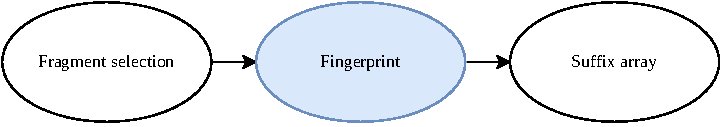
\includegraphics[width=0.8\textwidth]{figures/phases/phases_fingerprint.drawio.pdf}
    \end{center}
\end{figure}

\newsavebox{\firstlisting}
\begin{lrbox}{\firstlisting}
\begin{lstlisting}
public class Math() {
    public int multiplyByTwo(int param) {
        return param * 2;
    }

    public int addTwo(int param) {
        return param + 2;
    }
}
\end{lstlisting}
\end{lrbox}
\begin{figure}[htp]
	\begin{center}
        \subfloat[Source-code] {
            \usebox{\firstlisting}
        }
        \hspace{1cm}
        \subfloat[Fingerprint mapping] {
            \begin{tabular}{l | l}
                Token & Fingerprint \\
			    \hline
                public & 2 \\
                int & 3 \\
                multiplyByTwo & 4 \\
                ( & 5 \\
                param & 6 \\
                ) & 7 \\
                \{ & 8 \\
                return & 9 \\
                * & 10 \\
                2 & 11 \\
                ; & 12 \\
                \} & 13 \\
                addTwo & 14 \\
                + & 15 \\
            \end{tabular}
        }

        \vspace{0.5cm}
        \subfloat[Fingerprint, terminals underlined] {
            [ 2, 3, 4, 5, 3, 6, 7, 8, 9, 6, 10, 11, \underline{1}, 2, 3, 14, 5, 3, 6, 7,
            8, 9, 6, 15, 11, \underline{1}, \underline{0} ]
        }
	\end{center}
	\caption{Example fingerprint of Java source-code}
	\label{fig:fingerprint}
\end{figure}

The next phase of the algorithm is to transform the extracted tokens into a
representation which is less computationally heavy for the matching algorithm. The goal is
to reduce the total size of the input which needs to be processed.

Because the algorithm that is used for matching is based on an extended suffix array, the
representation should be in a format similar to a string, which is the standard input to a
suffix array construction algorithm. However, it is not strictly necessary to use strings.
The essential property of the input array is that we have a sizeable alphabet where each
element is comparable. The required size of the alphabet is correlated with the number of
unique token values in the code base. Therefore, it is safe to say that a larger code base
requires a larger alphabet, as larger code bases will generally have more unique token
values. We will use an array of integers instead of a string as it has a large alphabet in
most programming languages. The size of the alphabet of \verb|int| values in Java is large
enough that it will not be the limiting factor for how large code bases can be analyzed.

The algorithm utilizes fingerprinting in order to reduce the size of the representation.
Fingerprinting is a technique which involves taking some part of the input and mapping it
to a smaller bitstring, which uniquely identifies that part. In this case, the algorithm
takes each token extracted in the last phase, and maps its token value to the bitstring of
an integer. The algorithm stores and increments a counter, which is used to fingerprint a
token value whenever a new unique token is found. The mapping therefore starts with small
integers, and uses larger and larger integers as more unique token values are encountered.
The algorithm also stores a map from the token value, to the fingerprint value, which is
used to map multiple occurrences of the same token value to the same fingerprint value.

Figure \ref{fig:fingerprint} shows how a sample Java program would be fingerprinted. Note
that in the example only the tokens of the methods were extracted, which is why the class
declaration is not fingerprinted. The fingerprint mapping initializes its counter at 2 to
make space for some terminating characters. Each fragment is terminated by a $1$ and the
fingerprint is ultimately terminated by a $0$. Having these values in the fingerprint will
be useful for the matching algorithm where the suffix array is constructed and utilized
for detection. The fingerprint of each fragment is stored in the relevant document object.

\subsection*{Type-2 clones}

With the above fingerprinting algorithm, only type-1 clones would be detected. However,
CCDetect-LSP can detect type-2 clones if the client configures which token types should be
normalized. As shown in \cref{lspimplementation}, CCDetect-LSP can take a list of
\verb|blind_nodes| in its configuration, which signalizes CCDetect-LSP that each token
with a type which occurs in this list should be fingerprinted with the same value. This is
done by fingerprinting the token type, instead of the token value. For example in Java, if
the \verb|identifier| token is set as a token to normalize, then the \verb|param|
variables in figure \ref{fig:fingerprint} would be fingerprinted as \verb|identifier|,
instead of \verb|param|. This allows blind, but not consistent type-2 clone detection, as
we do not introduce any consistency here. With this fingerprint normalization, we can
continue on as if we are only detecting exactly similar fragments, since any instance of a
normalized token, will have the same value in the fingerprint.

\section{Suffix array construction}

\begin{figure}[H]
    \begin{center}
        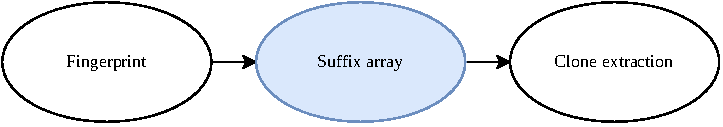
\includegraphics[width=0.8\textwidth]{figures/phases/phases_suffix.drawio.pdf}
    \end{center}
\end{figure}

The next step is to input the fingerprint into a suffix array construction algorithm
(SACA), so that the suffix array can be used to find repeating sequences. Recall that the
suffix array of a string sorts all the suffixes of the string, as discussed in
\cref{prelimalgos}. This makes it simple to find similar regions of text, since the most
similar suffixes will be adjacent in the suffix array. All the fingerprints which are
stored in each document object will now be concatenated to be stored in a single integer
array (with terminators after each fragment), which the suffix array (SA), inverse suffix
array (ISA) and longest-common prefix array (LCP) is computed from.

We have utilized a straight-forward implementation of the ``Induced sorting
variable-length LMS-substrings'' algorithm~\cite{LinearTimeSuffixArraySAIS} which computes
a suffix array in linear time. The following section will give a high-level overview of
how the algorithm works. 

The algorithm will be assumed to have a string as its input, as this is most common for
suffix arrays, and working with strings can be more clear to the reader when considering
suffixes. The algorithm is still applicable to our fingerprint, since an array of integers
will work similarly to a string when given as input.

The ``Induced sorting variable-length LMS-substrings'' algorithm (SA-IS) is an algorithm
that works by divide and conquering the suffix array and inducing how to sort the suffixes
of the string $S$ from a smaller string, $S_1$. This smaller string consists of the
``building blocks'' of $S$ and will make it simple to compute the rest of the suffix array
of $S$. First, we will introduce some definitions and theorems used for the algorithm.

\begin{definition}[L-type and S-type suffixes] A suffix starting at position $i$ in a
    string $S$ is considered to be L-type if it is lexicographically larger than the next
    suffix at position $i + 1$, meaning $\mathrm{suffix}(S, i) > \mathrm{suffix}(S, i+1)$.
    Conversely, a suffix is considered to be S-type if $\mathrm{suffix}(S, i) <
\mathrm{suffix}(S, i+1)$. The sentinel suffix (\$) of $S$ is always S-type.
\end{definition}

Note that two suffixes in the same string cannot be lexicographically equal, therefore all
cases are handled by this definition. Determining the type of each suffix can be done in
$O(n)$ time by scanning $S$ from right-to-left and observing the following properties:
$\mathrm{suffix}(S, i)$ is L-type if $\ArrayAccess{S}{i} > \ArrayAccess{S}{i + 1}$.
Similarly, $\mathrm{suffix}(S, i)$ is S-type if $\ArrayAccess{S}{i} < \ArrayAccess{S}{i +
1}$. If $\ArrayAccess{S}{i} = \ArrayAccess{S}{i + 1}$, then $\mathrm{suffix}(S, i)$ has
the same type as $\mathrm{suffix}(S, i + 1)$. This is true because if the first character
of the current suffix is not equal to first character of the next suffix, we already know
the type based on the first character. If the first character is equal, we have
effectively transformed the problem to finding the type of the next suffix, since we are
now comparing the second character of the current suffix, with the second character of the
second suffix. Since we have already computed the type of the next suffix, we can reuse
the value. Figure \ref{eq:suffixtypesrecurrence} shows a recurrence which determines the
type of each suffix in a string in $O(n)$ time and table \ref{tab:suffixtypesbanana} shows
an example.

\begin{figure}[t]
    \begin{center}
	$$
        type(S, i) =
        \begin{cases}
            \text{S-type} & \textrm{if\ i\ is\ the\ last\ character\ of\ S} \\
            \text{S-type} & \textrm{if\ } \ArrayAccess{\Var{S}}{\Var{i}} < \ArrayAccess{\Var{S}}{\Var{i + 1}} \\
            \text{L-type} & \textrm{if\ } \ArrayAccess{\Var{S}}{\Var{i}} > \ArrayAccess{\Var{S}}{\Var{i + 1}} \\
            type(S, i + 1) & \textrm{if\ } \ArrayAccess{\Var{S}}{\Var{i}} = \ArrayAccess{\Var{S}}{\Var{i + 1}} 
        \end{cases}
	$$

	\caption{Suffix type}
	\label{eq:suffixtypesrecurrence}
    \end{center}
\end{figure}

\begin{table}[t]
    \begin{center}
        \begin{tabular}[c]{l l l l l l l}
            B & A & N & A & N & A & \$ \\ 
            L & \underline{S} & L & \underline{S} & L & L & \underline{S} \\ 
            0 & 1 & 2 & 3 & 4 & 5 & 6 \\ 
        \end{tabular}
    \end{center}
    \caption{Suffix types of S = BANANA\$, LMS characters underlined}
    \label{tab:suffixtypesbanana}
\end{table}

\begin{definition}[LMS character]

    An LMS (Left-most S-type) character in a string $S$ is a position $i$ in $S$ such that
    $S[i]$ is S-type and $S[i-1]$ is L-type. An LMS-suffix is a suffix in $S$ which begins
    with an LMS character. The final character of $S$ (the sentinel) is always an LMS
    character and the first character is never an LMS character.

\end{definition}

\begin{definition}[LMS-substring]

    An LMS-substring in a string $S$ is a substring $S[i..j]$ in $S$ such that $i \neq j$,
    $S[i]$ and $[j]$ are LMS characters and there are no other LMS characters between. The
    sentinel character is also an LMS-substring and is the only LMS-substring of length
    $< 3$

\end{definition}

LMS-substrings are mostly lexicographically decreasing or increasing, which is easier to
sort. Table \ref{tab:bucketinglms} shows that in the string BANANA\$ there are 3 S-type
suffixes and all of them form LMS-substrings (ANA, ANA\$, \$). With these definitions, the
following theorems will allow us to induce the suffix array in linear time.

\begin{theorem}

    Given sorted LMS-suffixes of $S$, the rest of the suffix array can be induced in linear
    time. 

\end{theorem}

\begin{theorem}
    There are at most $n / 2$ LMS-substrings in a string $S$ of length n.
\end{theorem}

These theorems are proven in the original paper~\cite{LinearTimeSuffixArraySAIS}, these
theorems will now be used to compute the suffix array in linear time. Table
\ref{tab:bucketinglms} shows a running example. The smaller string is construced $S_1$ by
first sorting the LMS-substrings. Note that in this algorithm, we are not sorting suffixes
and substrings, but integers of the positions of those suffixes and substrings in $S$.
Sorting LMS-substrings can be done by first bucketing each LMS-substring by its first
character. The buckets are implemented as a single array with pointers to the head and
tail of each bucket, where the pointers are computed in linear time. Each LMS-substring is
inserted at the end of the correct bucket. Afterwards, L-type suffixes are bucketed by
iterating over the bucket array, and for each suffix, bucket the suffix to the left of it
in $S$, if it is L-type. Meaning that if we encounter a 6 when iterating over the bucket
array, the suffix at position 5 is bucketed, if it is L-type. These suffixes should be
bucketed at the head of their bucket. Finally, S-type suffixes are bucketed, but the
bucket array is now scanned from right-to-left and when encountering values where the
previous suffix is S-type, the previous suffix is bucketed at the tail of its bucket. This
final step could possibly change the ordering of the LMS-substrings. This procedure can be
interpreted as an initial attempt at building the suffix array, where the only thing we
know is that the LMS substrings are inserted in the correct ordering, which is proven in
the original paper~\cite{LinearTimeSuffixArraySAIS}. 

\begin{table}[t] \begin{center}
		\begin{tabular}[c]{r|cccc} Buckets & \$           & A            & B & N \\ Initial & \{ -1 \} & \{ -1, -1,
               -1 \}               & \{ -1 \}     & \{ -1, -1 \}         \\ Slot LMS & \{  6 \} & \{ -1,  3,  1 \} & \{ -1
               \}                  & \{ -1, -1 \}                        \\ Slot L-type & \{  6 \} & \{  5,  3,  1 \} & \{  0 \} & \{  4, 2
               \}                                                        \\ Slot S-type & \{  6 \} & \{  5,  3,  1 \} & \{  0 \} & \{  4,  2 \}\\\end{tabular}

		\vspace{0.25cm}
		\begin{tabular}[c]{r|c|c}
			        & \$    & 0 \\
			Mapping & ANA\$ & 1 \\
			        & ANA   & 2 \\
		\end{tabular}

		\vspace{0.25cm}

		\begin{tabular}[c]{l|c}
			$S_1$                 & $210$       \\
			SA of $S_1$           & $[2, 1, 0]$ \\
			Sorted LMS-substrings & $[6, 3, 1]$ \\
		\end{tabular}

	\end{center}
	\caption{Building $S_1$ and sorting LMS-substrings of S = BANANA\$}
	\label{tab:bucketinglms}
\end{table}

After sorting, each LMS-substring is given a unique increasing integer value. If there are
multiple equal LMS-substrings, these are given the same value. Two LMS-substrings are
considered equal if they are equal in terms of length, characters and types. $S_1$ is now
built by mapping each LMS-substring to its unique value, and concatenating them in the
original ordering. $S_1$ is now a smaller case which the algorithm recurses on. The string
is at most $n / 2$ in size, meaning there will be at most $\log_2(n)$ recursive calls. The
recursive call will return the suffix array of the $S_1$. The original paper proves a theorem
which shows that sorting $S_1$ is equivalent to sorting the LMS suffixes of $S$.
Therefore, the suffix array of $S_1$ can be mapped to the LMS suffixes of
$S$~\cite{LinearTimeSuffixArraySAIS}.

The base-case of the recursion occurs when the suffix array can be computed only by
bucketing each suffix, which occurs when each suffix starts with a unique character. 

Table \ref{tab:bucketinglms} shows how the LMS-substrings are bucketed and how $S_1$ is
constructed. We see that the final buckets are actually equal to the final SA which we are
trying to compute. This is because the LMS-substrings are already sorted in reverse order,
which is not true for any arbitrary input. $S_1$ consists of only unique characters,
therefore the suffix array of $S_1$ is computed by simply bucketing each suffix and
returning the array.

When the recursive call returns, the SA of $S_1$ is used to infer the order which the
LMS-suffixes should be slotted into the bigger SA. By scanning the smaller SA and mapping
those indices back to the indices of the original LMS-substrings, we get a sorted ordering
of the LMS-suffixes. We then scan the sorted LMS-suffixes from right-to-left and slot each
LMS-suffix at the end of its bucket, the rest of the L-type and S-type suffixes will be
slotted correctly afterwards. For BANANA\$ this will be the exact same process as in table
\ref{tab:bucketinglms}, since the LMS-substrings were already inserted in reverse
ordering.

There will be $O(\log_2(n))$ recursive calls, where each recursive call takes $O(n)$ time,
with $n$ halving in each call. Therefore, the recurrence will have the complexity of:

\vspace{-0.5cm}
\begin{gather*}
    T(n) =
\begin{cases}
    O(n) & \text{if base-case.} \\
    T(n / 2) + O(n) & \text{otherwise.}
\end{cases}
\end{gather*}
\vspace{-0.5cm}

Which means $T(n) = 2n = O(n)$.

\subsection*{Building ISA and LCP arrays}

Computing the ISA after constructing the SA is simple. Since the ISA is simply the inverse
of SA, it can be constructed in linear time with a single loop as seen in Algorithm
\ref{alg:isa}.

\begin{algorithm}[t]
  \SetAlgoLined\DontPrintSemicolon
    \algo{\ComputeISA{SA}}{
    $\Var{n} \gets \Len{$\Var{SA}$}$ \\
    $\Var{ISA} \gets \mathrm{array\ of\ size\ n}$

        \For{$\Var{i} \From 0 \To \Var{n}$}{
            $\ISA{\SA{i}} \gets \Var{i}$
        }

        \Return $\Var{ISA}$
    }

  \vspace{0.5cm}
  \caption{Compute ISA from SA}
  \label{alg:isa}
\end{algorithm}


Computing the LCP in linear time is more complicated and requires some insight about which
order to compute LCP values. We will also add one extra restriction to the LCP values,
being that the LCP values cannot match past a $1$, which were the terminal value between
fragments. This restriction will be useful when we want to extract clones using the LCP
array. The algorithm to compute the LCP is shown in Algorithm \ref{alg:lcp}.  The
intuition for this algorithm is that if a suffix at position $i$ in $S$ has an LCP value
$l$ describing the common-prefix between it and some other suffix at position $j$ in $S$,
then the LCP value of the suffix at position $i + 1$ is at least $l - 1$, since there
exists suffixes at position $i + 1$ and $j + 1$ which shares at minimum $l$ characters,
except for the first character which is now cut off. Therefore, they share at least $l -
1$ characters, and the algorithm can start comparing the characters at that offset. Table
\ref{tab:lcpexample} shows an example where the suffixes at position $2$ and $4$ have a
minimum LCP value of $2$, because the suffixes at position $1$ and $3$ have a common
prefix of length $3$.

Now that we have computed the extended suffix array in linear time, we are ready to detect
clones in our code base using this data structure.

\begin{algorithm}[t]
  \SetAlgoLined\DontPrintSemicolon
    \algo{\ComputeLCP{S, SA, ISA}}{
        $\Var{n} \gets \Len{$\Var{SA}$}$

        $\Var{LCP} \gets \mathrm{array\ of\ size\ n}$

        $\Var{lcpLen} \gets 0$

        \For{$\Var{i} \From 0 \To \Var{n} - 1$}{
            $\Var{r} \gets \ISA{i}$

            $\Var{prevSuffix} \gets \SA{\Var{r} - 1}$

            \While{$\ArrayAccess{\Var{S}}{\Var{i} + \Var{lcpLen}} =
            \ArrayAccess{S}{\Var{prevSuffix} + \Var{lcpLen}} \And \ArrayAccess{S}{\Var{i} +
        \Var{lcpLen}} \neq 1$}{
                $\Var{lcpLen} \gets \Var{lcpLen} + 1$
            }

            $\LCP{\Var{r}} \gets \Var{lcpLen}$

            $\Var{lcpLen} \gets \Max{$0, \Var{lcpLen} - 1$}$
        }

        \Return ISA
    }

  \vspace{0.5cm}
  \caption{Compute LCP from input string S, SA, and ISA}
  \label{alg:lcp}
\end{algorithm}

\begin{table}[t]
    \begin{center}
        \begin{tabular}[c]{c|cccccc|c}
            Index & \multicolumn{6}{c}{Suffix} & Minimum LCP \\
            \hline
            1 & A & N & A & N & A & \$ & 0 \\ 
            3 & A & N & A & \$ &  &  & 0\\ 
            2 & N & A & N & A & \$ & & 2 \\ 
            4 & N & A & \$ & & &  & 2\\ 

        \end{tabular}
    \end{center}
    \caption{Minimum common LCP values between suffixes for S = BANANA\$}
    \label{tab:lcpexample}
\end{table}

\section{Clone extraction}

\begin{figure}[H]
    \begin{center}
        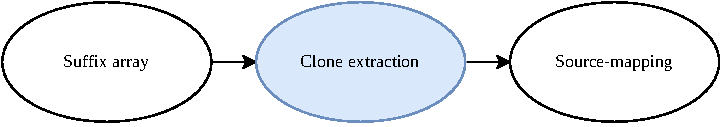
\includegraphics[width=0.8\textwidth]{figures/phases/phases_cloneextraction.drawio.pdf}
    \end{center}
\end{figure}

With the extended suffix array computed, we can now consider which substrings (prefixes of
suffixes) we want to extract as potential code clones. In this phase, the indices of the
fingerprint which we consider to be code clones are extracted, which will be mapped back
to the original source code in the next phase.

\begin{algorithm}[t]
  \SetAlgoLined\DontPrintSemicolon
    \algo{\SimpleCloneExtraction{S, ISA, LCP}}{
        $n \gets \Access{S}{len}$ \;
        $\Var{clones} \gets \Var{list}$ \;


        \For{$i \From 0 \To n - 1$}{
            \If{$\ISA{\Var{i}} = 0$}{
                \Continue \;
            } \;

            \If{$\LCP{\ISA{\Var{i}}} \geq \text{THRESHOLD}$}{
                $\Insert{$\Var{clones}, \Var{i}$}$ \Comment{Adds i to the clone-list}
            }
        }

        \Return clones
    }

  \vspace{0.5cm}
  \caption{Extract clones indices in a string $S$}
  \label{alg:simplecloneextraction}
\end{algorithm}

\begin{algorithm}[t]
  \SetAlgoLined\DontPrintSemicolon
    \algo{\CloneExtraction{S, ISA, LCP}}{
        $\Var{n} \gets \Access{\Var{S}}{\Var{len}}$ \;
        $\Var{clones} \gets \textrm{empty\ list}$ \;


        \For{$\Var{i} \From 0 \To \Var{n} - 1$}{
            \If{$\ArrayAccess{\Var{ISA}}{i} = 0$}{
                \Continue \;
            } \;

            \If{$\ArrayAccess{\Var{LCP}}{\ArrayAccess{\Var{ISA}}{\Var{i}}}  \geq \Var{THRESHOLD}$}{
                $\Insert{$\Var{clones}, \Var{i}$}$ \tcp{Adds i to the clone-list} \;


                \While{$\Var{i} + 1 < \Var{n} \And
                \ArrayAccess{\Var{LCP}}{\ArrayAccess{\Var{ISA}}{\Var{i} + 1}} <
            \ArrayAccess{\Var{LCP}}{\ArrayAccess{\Var{ISA}}{\Var{i}}}$}{
                    $\Var{i} \gets \Var{i} + 1$
                }

            }
        }

        \Return $\Var{clones}$
    }

  \vspace{0.5cm}
  \caption{Extract clones indices in a string $S$, ignoring contained clones}
  \label{alg:cloneextraction}
\end{algorithm}

A straightforward solution is to extract every suffix which has an LCP value which is
greater than the token threshold. The algorithm is a loop over $S$, using ISA to find the
corresponding LCP value. This finds the clone indices, as shown in Algorithm
\ref{alg:simplecloneextraction}.


However, this algorithm will return a lot of contained clones. A contained clone is a
clone where all the tokens of the clone is a part of another, larger clone. The algorithm
will give a lot of contained clones, for example in the case where there is a suffix with
an LCP value of $100$, the next suffix will have the LCP value of at least $99$ and likely
matches with the same code clone as the previous suffix, but with an offset of 1 token.
For any large code clone, there will therefore be many smaller clones which are completely
contained within it, but these clones are also likely to match with another clone which is
also contained within the larger clones match. Since the code clones point at mostly the
same area, the contained clones are not very useful, and is discarded by the tool. We
extend our clone extraction algorithm to account for this, by using the following theorem:

\begin{theorem} 

    The LCP of a suffix at position $i$ is completely contained in the LCP of the previous
    suffix at position $i - 1$ if the LCP value of the suffix at position $i - 1$ is
    greater than the LCP value of the suffix at position $i$. Meaning $\LCP{\ISA{\Var{i}}}
    < \LCP{\ISA{\Var{i} - 1}}$.


\end{theorem}


Algorithm \ref{alg:cloneextraction} adds a while-loop to the clone extraction algorithm
which skips over suffixes which are contained according to the theorem. Note that this
algorithm doesn't disallow contained clones entirely, but any clone which is a shorter
version of another clone pointing to the same match, will be discarded. Also note that
overlapping clones, meaning two clones which share tokens, but where neither contains the
other, will not be filtered.

At the end of this phase we now have a list of indices in the fingerprint which is
considered to be code clones.

\section{Source-mapping}

\begin{figure}[H]
    \begin{center}
        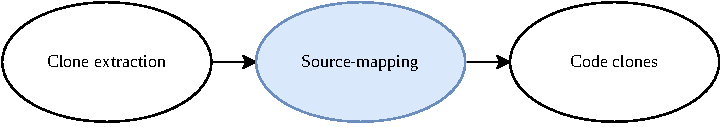
\includegraphics[width=0.8\textwidth]{figures/phases/phases_sourcemap.drawio.pdf}
    \end{center}
\end{figure}

With the clone indices in the fingerprint computed, we are almost finished. The final step
is to map the clone indices back to the original source code. This is the phase where
clone objects are built. Clone objects consist mainly of the source-mapping information,
and a list of other code clones which it matches to. In order to correctly identify where
a clone is located, we need to know which file the clone is located in, the range of the
source code in that file the code clone covers, and the other matching code clones.

To accomplish this, each document in the index needs to store the range of each of its
tokens and keep track of which portion of the fingerprint the tokens of the document is
located. This is done by storing two integer variables, each storing the start position
and end position that the document has in the fingerprint. 

\begin{algorithm}[t]
  \SetAlgoLined\DontPrintSemicolon
    \algo{\SourceMap{documents, i}}{
        $\Var{left} \gets 0$ \;
        $\Var{right} \gets \Len{$\Var{documents}$} - 1$ \;\;


        \While{$\Var{left} \leq \Var{right}$}{
            $\Var{mid} \gets (\Var{left} + \Var{right}) / 2$

            \uIf{$\Access{\ArrayAccess{\Var{documents}}{\Var{mid}}}{\Var{end}} < i$}{
                $\Var{left} = \Var{mid} + 1$
            }
            \uElseIf{$\Access{\ArrayAccess{\Var{documents}}{\Var{mid}}}{\Var{start}} > i$}{
                $\Var{right} = \Var{mid} - 1$
            }
            \Else {
                $\Var{D} \gets \ArrayAccess{\Var{documents}}{\Var{mid}}$ \;
                $\Var{range} \gets \ArrayAccess{\Access{\Var{D}}{\Var{ranges}}}{\Var{i} -
                \Access{\Var{D}}{end}}$

                \Return $(\Access{\Var{D}}{\Var{uri}}, \Var{range})$
            }

        }
    }

  \vspace{0.5cm}
  \caption{Get source-map for a position $i$ in the fingerprint}
  \label{alg:sourcemap}
\end{algorithm}

To determine which document a fingerprint position corresponds to, we can perform a binary
search on the list of the documents, which is sorted based on the start position of the
documents fingerprint. The goal is to find the document $D$ where the fingerprint position $i$
is 

$$
\Access{D}{start} \leq i \leq \Access{D}{end}
$$

Once the correct document has been found, we simply have to look up the correct range of
the token which the fingerprint index corresponds to, which the document stores. The index
of this range is $i - \Access{D}{start}$.

Algorithm \ref{alg:sourcemap} returns the source-map of a given position $i$ in the
fingerprint, which includes the URI for the document and the source code range of the
token at position $i$.

This algorithm only shows how to look up the position of a single token. Since a code
clone is a range between two tokens, we have to look up the position at index $i$
extracted in the previous phase, and the position where the clone ends, which is index $i
+ \text{LCP}[\text{ISA}[i]]$. The range of the code clone is therefore the combination of
the starting range of the first token (at position $i$) and the ending range of the second
token (at position $i + \text{LCP}[\text{ISA}[i]]$):

\subsection*{Aggregating clones}

With this algorithm which gets the clone locations, the next step is to make sure that
matching code clones are collected into buckets of clone classes. Remember that the LCP
array only gives us the longest match between two suffixes, but it is naturally possible
to have more than two clones of the same code snippet. This case happens when multiple
consecutive indices in the SA are considered to be clones. Since we only look for type-1
(and type-2 clones if token types are normalized), the transitivity property holds,
meaning that if

$$
SA[i] \xrightarrow{clone} SA[i+1] \xrightarrow{clone} SA[i + 2]
$$

then clones at position $SA[i]$ and $SA[i + 2]$ are clones as well. This should be
achieved by making sure that every new clone-pair discovered adds previously detected
clones to their clone sets, and previously discovered clones also add new clones to
theirs. Figure \ref{fig:cloneaggregation} shows how a new match is found in two previously
disjoint clone classes, and the resulting aggregated clone class.

This is achieved in algorithm \ref{alg:buildclonemap} where we build a clone-map, where
the key is the index that a clone starts in the fingerprint, and the value is a code clone
object. For each clone index $i$ which was extracted in the last phase, we get the
corresponding match index $j$ ($\text{SA}[\text{ISA[i]} - 1]$), and for both $i$ and $j$
we look in the clone-map if there already is a clone at that position, or a new clone
object is created and put in the map. Then, in order to aggregate the previously
discovered clones and the new clone together, the set of matching clones is unioned
between the two clones. In this way, all the previous existing clones of $i$ is added as a
clone in $j$ and vice versa. Every clone in the two clone classes will then receive the
same set of code clones. The \verb|UnionCloneClass| function unions all the clone sets in
both clone classes and then adds a match from all clones in one clone class to all clones
in the other.

Finally, we have a list of every code clone in the code base, which is then sent to the
LSP module of the tool, which handles the displaying of code clones to the client as
shown in \cref{lspimplementation}.

\begin{figure}[t]
    \begin{center}
        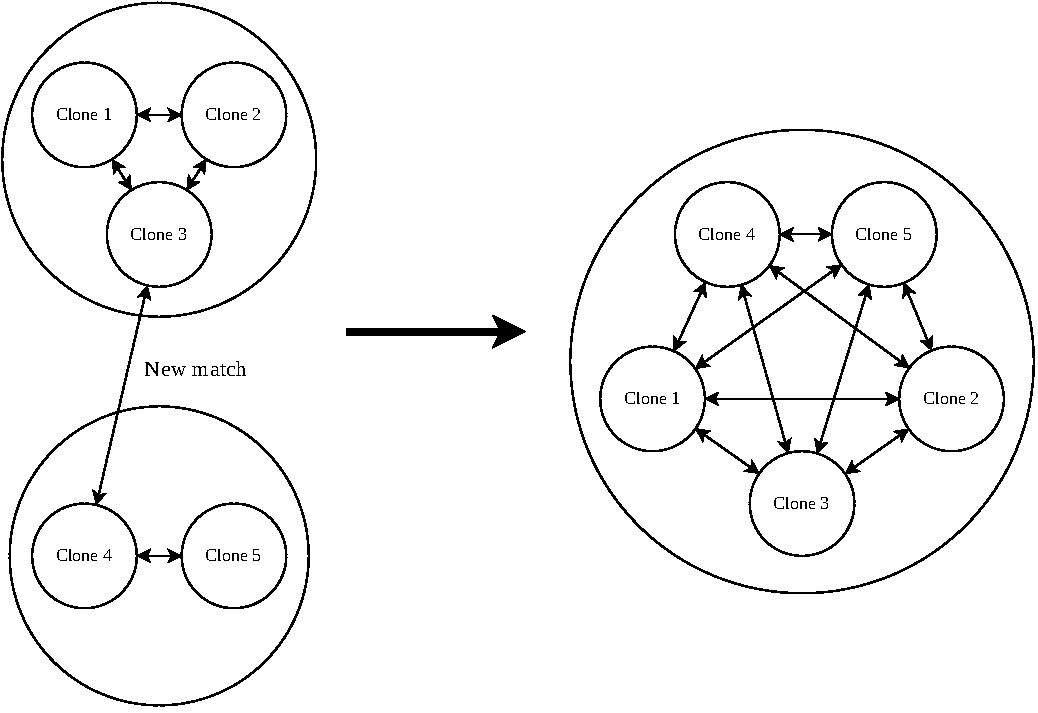
\includegraphics[width=0.95\textwidth]{figures/cloneaggregation.drawio.pdf}
    \end{center}
    \caption{Clone class aggregation when a new match is found}
    \label{fig:cloneaggregation}
\end{figure}

\begin{algorithm}[t]
  \SetAlgoLined\DontPrintSemicolon
    \algo{\GetCloneMap{index, cloneIndices}}{
        $\Var{n} \gets \Access{\Var{cloneIndices}}{\Var{len}}$ \;
        $\Var{cloneMap} \gets \textrm{Empty map with type: } \Var{int} \rightarrow \Var{CodeClone}$ \;\;

        
        \For{$\Var{i} \From 0 \To \Var{n} - 1$}{
            $\Var{firstIndex} \gets \ArrayAccess{\Var{cloneIndices}}{\Var{i}}$ \;
            $\Var{secondIndex} \gets \SA{\ISA{\Var{firstIndex}} - 1}$ \;
            $\Var{size} \gets \LCP{\ISA{\Var{firstIndex}}} - 1$ \;\;


            \Comment{Use SourceMap function to get ranges and documents of clones}
            $\Var{firstRange} \gets \textrm{Get source between firstIndex and
            (firstIndex + size)}$ \;
            $\Var{secondRange} \gets \textrm{Get source between secondIndex and
            (secondIndex + size)}$ \;\;

            $\Var{firstDocument} \gets \Access{\Var{firstRange}}{\Var{document}}$ \;
            $\Var{secondDocument} \gets \Access{\Var{secondRange}}{\Var{document}}$ \;\;
            
            \Comment{Build clone objects if they don't exist}
            \If{$\Var{firstIndex} \NotIn \Var{cloneMap}$}{
                $\Var{firstClone} \gets \New
                \CodeClone{$\Access{\Var{firstDocument}}{\Var{uri}},
                \Var{firstRange}$}$ \;
                $\Put{$\Var{cloneMap}, \Var{firstIndex}, \Var{firstClone}$}$ \Comment{Put
                clone with firstIndex as key}
            }
            \If{$\Var{secondIndex} \NotIn \Var{cloneMap}$}{
                $\Var{secondClone} \gets \New
                \CodeClone{$\Access{\Var{secondDocument}}{\Var{uri}},
                \Var{secondRange}$}$ \;
                $\Put{$\Var{cloneMap}, \Var{i}, \Var{secondClone}$}$ \Comment{Put
                clone with secondIndex as key}
            } \;

            \Comment{Union clone classes}
            \UnionCloneClass{\Get{$\Var{cloneMap}, \Var{firstIndex}$}, \Get{$\Var{cloneMap,
            \Var{secondIndex}}$}} \;
        }
        \Return $\Var{cloneMap}$
    }

  \vspace{0.5cm}
  \caption{Build clone-map given the clone indices in the fingerprint}
  \label{alg:buildclonemap}
\end{algorithm}

\chapter{Implementation: Incremental detection}
\label{dynamicdetection}

The following chapter will present the incremental algorithm which efficiently updates the
list of clones, without having to rebuild the full extended suffix array. Given an edit to
a file in the project, we will be able to update the document index, fingerprint, extended
suffix array and list of clones faster than the initial detection.

The incremental algorithm is run whenever a document is changed. The document index is
signalized of a change either when a file is saved, or on any keystroke, configurable by
the client. 

In broad strokes, when a file is changed, we will first update the document index, which
involves also incrementally parsing the changes to the file. From there we want to
determine which edits have happened to the fingerprint, which we compute with an edit
distance algorithm. The edits are the input to the dynamic extended suffix array
algorithm, which is updated to reflect the extended suffix array of the new fingerprint.
Afterwards, the clones are extracted from the extended suffix array similarly to the
initial detection, but with slight optimizations based on storing positions of potential
clone locations between revisions.

\section{Affordable operations}

Before discussing the algorithm, it is useful to determine the time cost associated with
different operations and discuss what operations we can afford. The baseline we are
comparing against is the initial detection where everything is computed from scratch,
which runs in linear time in the size of the code base and fingerprint. We are therefore
only looking to perform operations which are less computationally heavy than a linear scan
over the code base. We can for example afford to iterate over the contents of a single
file, which will be useful for our algorithm. 

We cannot afford to iterate over the entire code base, meaning the contents of all files
in the code base. The initial detection takes linear time in the size of the code base,
therefore, iterating over the entire code base will likely make the algorithm as slow as
the initial detection. The same goes for the iterating over the entire fingerprint.

As mentioned, we can afford to iterate over the contents of a single file. Iterating over
the contents of a file with up to a few thousands lines is not a very expensive operation
to perform and will not take a significant amount of time. The whole string of the file
contents will be needed for Tree-sitter to incrementally parse the file.

Parsing an entire file however, can be too expensive in some cases. While the running time
of parsing a single file is still linear in the size of file content, parsing a large file
from scratch can take a significant amount of time in practice, and for small code bases
with large files, parsing can take a significant portion of the total running time of an
incremental update. This is why incremental parsing with Tree-sitter is used, which lowers
the runtime closer to $O(\vert\text{edit}\vert)$, rather than $O(\vert \text{file} \vert)$

We can also afford two more useful operations, iterating over the documents in the index
(not their contents), and iterating over the clones. We can afford to do these operations
because the number of documents and the number of clones is likely multiple magnitudes
smaller than the contents of the entire code base. Iterating over the documents will be
useful when we are updating the document index, and iterating over the clones is necessary
to do when the clones are mapped back to their original source code locations.

Why we can afford these operations will be become clearer in \cref{evaluation}, the main
idea is that all the operations we can afford will take an insignificant amount of time
compared to updating the extended suffix array.

\section{Updating the document index}

\begin{figure}[H]
    \begin{center}
        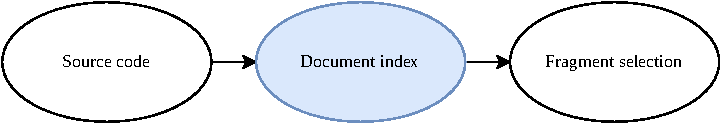
\includegraphics[width=0.8\textwidth]{figures/phases/phases_documentindex.drawio.pdf}
    \end{center}
\end{figure}

The first step of the incremental algorithm is to update the document index. We will also
look at how we can reduce the memory usage of the index without a loss in terms of time
complexity.

Each document stores its own content, AST and fingerprint. It is not strictly necessary to
store either the content or the AST in memory all the time, as it is likely that only a
handful of files are open in the IDE at once. Therefore, in the initial detection, we can
free the memory of the file content and AST for each document after the fingerprint has
been computed. However, if a file is opened in the IDE, the file can now be changed, so we
should facilitate efficient updates for these files at least. When a file is opened, the
file content should be read from the disk and updated via the
\verb|textDocument/didChange| messages sent from the client. It is also important to keep
the AST of the opened file in memory in order to facilitate incremental parsing of the
opened files. 

When a file is opened, the LSP client sends a \verb|textDocument/didOpen| message to the
server, which finds the relevant document $D$ in the index, and sets the following fields:

\begin{flalign*}
&\Access{D}{\Var{open}} = \True \\
&\Access{D}{\Var{content}} = \Read{$\Access{D}{\Var{uri}}$} \\
&\Access{D}{\Var{AST}} = \Parse{$\Access{D}{\Var{content}}$}
\end{flalign*}

After the document fields have been set, the document is ready to receive updates. When
the LSP client sends a \verb|textDocument/didChange| message, the message consists of the
URI of the edited file, the range of the content which has changed, and the content which
has potentially been inserted. This range is then used in a Tree-sitter incremental parse
of the file content. After this parse, we have efficiently updated a documents content and
AST. After this update, we also set $\Access{D}{\Var{changed}} = \True$.

\section{Updating fingerprints}

\begin{figure}[H]
    \begin{center}
        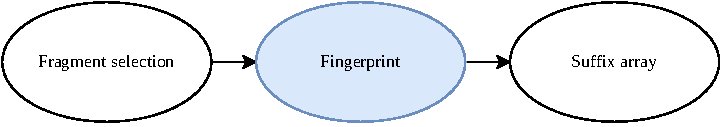
\includegraphics[width=0.8\textwidth]{figures/phases/phases_fingerprint.drawio.pdf}
    \end{center}
\end{figure}

With the updated AST for all documents, we can update the fingerprint of all documents
which have been changed. For each document $D$ where $\Access{D}{\Var{changed}} = \True$,
the fingerprint for $D$ may have changed. Computing the new fingerprint is the same
process as in the initial detection, where we first query the AST for all nodes of a
certain type, then for each matched node $N$, we extract and fingerprint all the tokens
which $N$ covers, using the same fingerprint mapping as was used for the initial
detection.

An additional change we have to consider when incrementally updating fingerprints is that
for a document $D$, $\Access{D}{start}$ and $\Access{D}{end}$ which corresponds to the
range which $D$ covers in the fingerprint, may have changed.  Also, any document $D_1$
where $\Access{D_1}{start} > \Access{D}{start}$ could also have its range changed. This
range needs to be updated in order for the source-mapping to work. This is solved while
updating each documents fingerprint by counting the number of tokens in each document
after updating, and setting the appropriate \verb|start| and \verb|end| fields.

Figure \ref{fig:fingerprintupdate} shows how an index of three documents is updated when
two tokens are inserted. Note that each document stores its own fingerprint, we do not
need to concatenate them to one large array as in the initial detection.

\begin{figure}[t]
    \begin{center}
        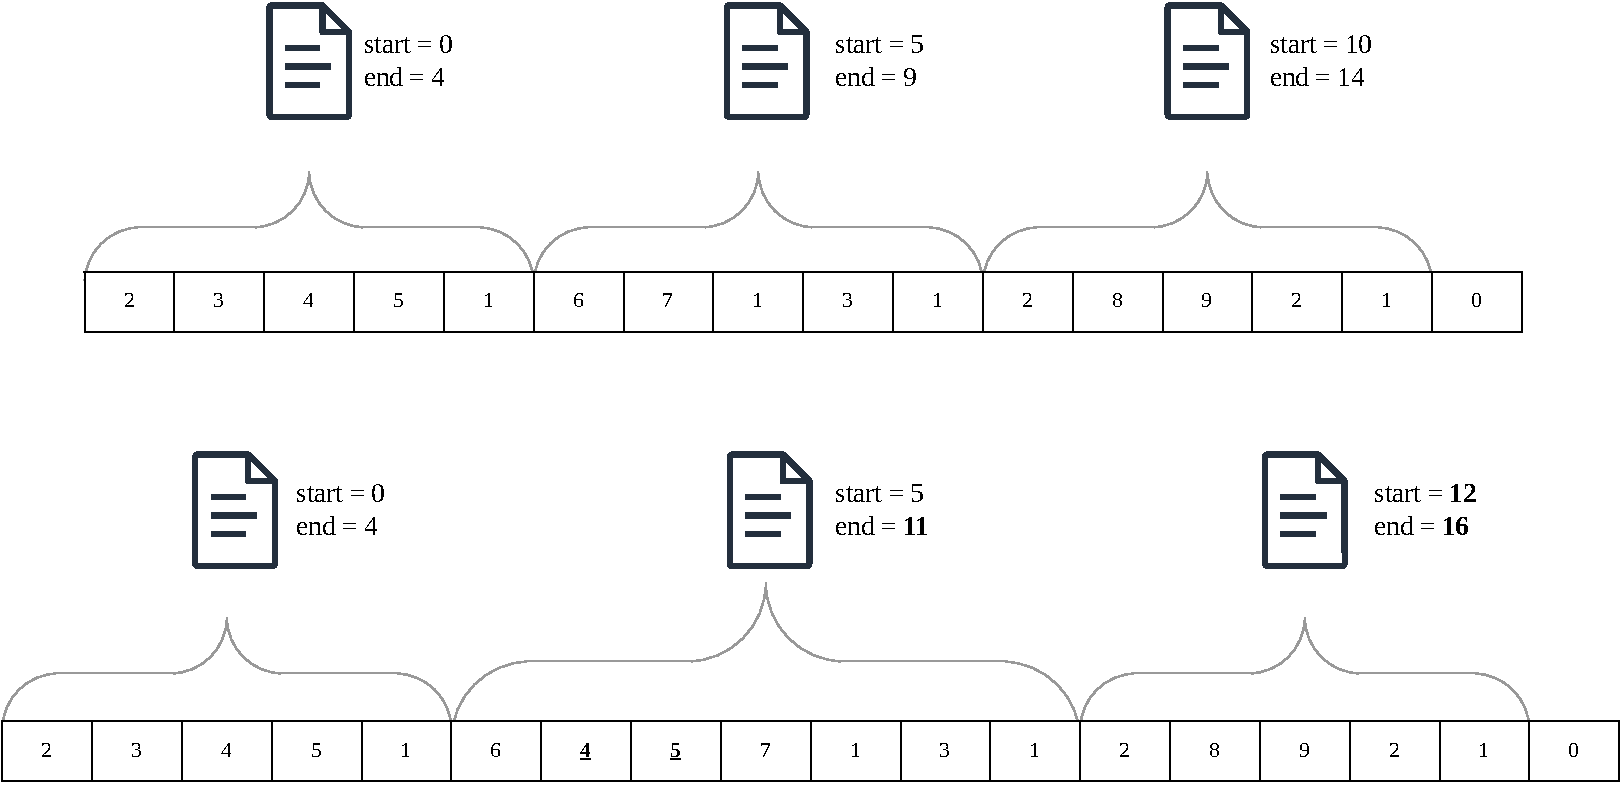
\includegraphics[width=0.95\textwidth]{figures/indexupdate.drawio.pdf}
    \end{center}
    \caption{Old (above) and new (below) fingerprints and ranges when two tokens are
    inserted.}
    \label{fig:fingerprintupdate}
\end{figure}

\section{Computing edit operations}

With the updated fingerprint, we could build the suffix array from scratch and already see
a substantial improvement in performance, as is shown in \cref{evaluation}. The major
bottleneck of the initial detection is to parse and fingerprint the entire code base. In
order to improve the algorithm even further, we will dynamically update the extended
suffix array to avoid recomputing it fully.

The input to the dynamic extended suffix array algorithm is a set of edit operations. An
edit operation can either be deleting, inserting or substituting a set of consecutive
characters in the fingerprint. The dynamic extended suffix array algorithm will take each
edit operation, and update its state to reflect the new fingerprint. Therefore, the first
problem to solve is to determine what exactly has changed in the fingerprint. 

There are a couple of approaches we could take to determine the edit operations. The
simplest is that whenever a file has changed, regard the entire file as changed, and
perform a delete operation which removes the entire fingerprint of that file, and then an
insertion which inserts the new fingerprint of that file. This is a simple approach which
can have decent performance if the file is small, but can also lead to unnecessarily large
edit operations. The fingerprint of the file is likely to be very similar to the previous
version, therefore deleting and inserting the entire fingerprint could be a lot more work
than it needs to be. However, this idea that we can always reduce the number of operations
to only two, a deletion and an insertion, will be useful in our final algorithm.

Another possible approach is to look at the ranges that the LSP client provides with each
\verb|textDocument/didChange| message and determine which tokens in the fingerprint have
been affected according to this range. However, this approach tightly couples the
algorithm to LSP and the scenario where we know the exact ranges of each change. Also, we
might do unnecessary amounts of operations if we do multiple edits, since some operations
could cancel each other out, for example by inserting and then deleting the same text.

A better approach is to determine the changes of the fingerprint using an edit distance
algorithm. An edit distance algorithm is an algorithm which computes the distance between
two strings $S_1$ and $S_2$. Distance between two strings is the minimum number of edit
operations (insert, delete, substitute) which is required to transform $S_1$ into $S_2$.
Many of the algorithms which computes the edit distance, also allows computing what the
operations are.

The classic algorithm for calculating edit distance operations is attributed to Wagner and
Fischer~\cite{WagnerFischer}. The input to the algorithm is two strings $S_1$ and $S_2$ of
length $n$ and $m$. The output will be the set of operations needed to turn $S_1$ into
$S_2$. This algorithm is based on dynamic programming where a matrix $M$ is filled from
top to bottom and then the operations are inferred from $M$. The recurrence in equation
\ref{eq:editdistancerecurrence} shows how the edit distance matrix is filled and table
\ref{tab:wagnerfischermatrix} shows an example matrix.

\begin{figure}[t]
    \begin{center}
	$$
		\sum^{n}_{i = 0}{M[i][0] = i}
	$$
	$$
		\sum^{m}_{j = 0}{M[0][j] = j}
	$$

	\begin{gather*}
		M[i][j] =
		\begin{cases}
			M[i-1][j-1] & \mathrm{if\ } S_1[i] = S_2[j] \\
            1 + \Min{$M[i-1][j-1], M[i][j-1], M[i-1][j]$}
		\end{cases}
	\end{gather*}
	\caption{Edit distance recurrence}
	\label{eq:editdistancerecurrence}
    \end{center}
\end{figure}

Each index $i, j$ in $M$ contains the edit distance value between the substrings
$\ArrayAccess{S_1}{0..i}$ and $\ArrayAccess{S_2}{0..j}$ The values in $M$ are calculated
by determining what is the cheapest operation to do at a certain location to make the
substrings equal. This can be determined by looking at the three surrounding indices in
$M$: $\MatrixAccess{M}{i - 1}{j - 1}$, $\MatrixAccess{M}{i - 1}{j}$ and
$\MatrixAccess{M}{i}{j - 1}$. Each of these indices equate to deleting, inserting or
substituting a character in $S_1$. 

\begin{table}
	\begin{center}
		\begin{tabular}[c]{c|c|c|c|c|c|c|c|c|c|}
			  &                      & D                    & E                    & M                    & O                    & C                    & R                    & A                    & T                    \\\hline
			  & \cellcolor{blue!25}0 & 1                    & 2                    & 3                    & 4                    & 5                    & 6                    & 7                    & 8                    \\\hline
			R & 1                    & \cellcolor{blue!25}1 & 2                    & 3                    & 4                    & 5                    & 5                    & 6                    & 7                    \\\hline
			E & 2                    & 2                    & \cellcolor{blue!25}1 & 2                    & 3                    & 4                    & 5                    & 6                    & 7                    \\\hline
			P & 3                    & 3                    & \cellcolor{blue!25}2 & 2                    & 3                    & 4                    & 5                    & 6                    & 7                    \\\hline
			U & 4                    & 4                    & \cellcolor{blue!25}3 & 3                    & 3                    & 4                    & 5                    & 6                    & 7                    \\\hline
			B & 5                    & 5                    & 4                    & \cellcolor{blue!25}4 & 4                    & 4                    & 5                    & 6                    & 7                    \\\hline
			L & 6                    & 6                    & 5                    & 5                    & \cellcolor{blue!25}5 & 5                    & 5                    & 6                    & 7                    \\\hline
			I & 7                    & 7                    & 6                    & 6                    & 6                    & \cellcolor{blue!25}6 & 6                    & 6                    & 7                    \\\hline
			C & 8                    & 8                    & 7                    & 7                    & 7                    & 6                    & \cellcolor{blue!25}7 & 7                    & 7                    \\\hline
			A & 9                    & 9                    & 8                    & 8                    & 8                    & 7                    & 7                    & \cellcolor{blue!25}7 & 8                    \\\hline
			N & 10                   & 10                   & 9                    & 9                    & 9                    & 8                    & 8                    & 8                    & \cellcolor{blue!25}8 \\\hline

			\hline
		\end{tabular}
	\end{center}
	\caption{Edit distance matrix for REPUBLICAN $\rightarrow$ DEMOCRAT}
	\label{tab:wagnerfischermatrix}
\end{table}


The edit operations can then be inferred from $M$ by backtracking from the bottom-right
index, to the top-left, giving us the edit operations in reverse. At each position $i, j$
we choose either of the 3 surrounding indices, the same indices which were used to
determine the value originally. Choosing the left index ($i, j - 1$) equates to inserting
the character $\ArrayAccess{S_2}{j - 1}$ at position $i - 1$. Choosing the top index ($i -
1, j$) equates to deleting the character $\ArrayAccess{S_1}{i - 1}$. Choosing the top-left
index ($i - 1, j - 1$) equates to substituting $\ArrayAccess{S_1}{i - 1}$ with
$\ArrayAccess{S_2}{j - 1}$. If these characters are already equal, the operation can be
ignored. For example in table \ref{tab:wagnerfischermatrix}, the first operation is to
substitute \verb|R| with \verb|D| at position $0$. Afterwards \verb|P| and \verb|U| is
deleted at position $2$. Then the \verb|B| which is now at position $2$ is substituted by
\verb|M|. This continues with more substitutions until we finally have \verb|DEMOCRAT|.

\subsection*{Aggregating edit operations}

In the next phase we will feed the edit operations into an algorithm which dynamically
updates our suffix array based on those operations. However, this algorithm will be more
efficient if the operations are combined to singular inserts, deletes or substitutes of
strings more than one character. The edit distance algorithm outputs only single character
operations, meaning we insert, delete or substitute a single character at a time. We
therefore want a way to combine these operations to ``larger'' operations.

We define an EditOperation with the following record:

\begin{lstlisting}
EditOperation {
    OperationType type,
    char[] chars,
    int position
}
\end{lstlisting}

where type is either an insert, delete or substitute.

One way to combine operations is to find operations of the same type which are sequenced
in the matrix. For example in table \ref{tab:wagnerfischermatrix}, we have two consecutive
delete operations, where \verb|P| and \verb|U| is deleted at position $2$. These two
operations could be combined to a single delete operation of two characters.

The idea for the algorithm which computes the edit operations is to traverse the optimal
matrix path backwards and for each operation we either append to the current operation if
possible, or start a new operation. We can continue the current operation if the next
operation is of the same type, and the next operation has the same position as the current
operation. For example in table \ref{tab:wagnerfischermatrix}, we have two delete
operations in a sequence at position $1$ where \verb|P| and \verb|U| is deleted. The first
operation we encounter is the deletion of \verb|U|. At this point we create a new
\verb|EditOperation| with position $1$ and \verb|U| in the \verb|chars| array. The next
operation is also a delete operation at position $1$, so we add the \verb|P| to the list
of characters for the operation to delete. The next operation is a substitute at position
$0$, so we cannot continue the delete operation, and a new substitute operation is created
instead. Similarly, at position $2$ to $5$, we substitute \verb|BLIC| with \verb|MOCR|.
This operation is computed in a backwards fashion similarly to how we did the deletion,
except that the position of the operation is decremented for each character we add to it.

Note that this algorithm is not an optimal algorithm, as this is a trade-off between
processing many characters in few operations, versus processing many operations with few
characters. As mentioned earlier, one could always reduce the solution to be only two
operations, deleting the whole string, and inserting the new string. This is only two
operations, but likely processes more characters in total compared to our algorithm. See
Appendix \ref{alg:wagnerfischeroperations} for detailed pseudocode of the algorithm
explained in this section.

\subsection*{Optimizing memory usage}

A problem with the above solution is the memory usage of the matrix. It is not feasible to
input the entire old and new fingerprint into an edit distance algorithm, as the full
fingerprint can have millions of symbols, and the old and new fingerprint is likely
approximately the same size. This would require a matrix which is too large to fit in
memory. We will use a few techniques to reduce the memory usage of this algorithm without
compromising on the time complexity.

The first technique is to not input the whole fingerprint. We can drastically reduce the
size of the input by only comparing the old and new fingerprint of the document $D$ which
has been edited. $D$ stores its previous and current fingerprint, and whenever it is
edited, we can compute the edit operations of $D$, with its previous and current
fingerprint as input. This also avoids having to construct the full fingerprint by
concatenating each documents fingerprint, which we had to do in the initial detection.
With this approach however, the position of each edit operation of $D$ will not have the
correct position relative to the entire fingerprint, so $\Access{D}{\Var{start}}$ is added
to the position of each edit operation to correct this.

Another optimization we can do to reduce the size of the matrix is to remove the
``trivial'' part at each end of our matrix. If we compare two strings which have many
similar characters at the beginning or end of our string, we know that these will not
produce any edit operations in the matrix, as they will simply be diagonal moves
(substitutes) where the characters are already the same. In table
\ref{tab:minimizededitmatrix} we see the edit matrix for the input \verb|FASCINATING| and
\verb|FINISHING|. The two words share the common prefix \verb|F| and the common suffix
\verb|ING|. If we examine the edit distance values, we see that the highlighted green
matrix starts at $0$ in the top left, and ends with $6$ in the top right, which is the
same final values as in the full matrix. Also, we see that there are no edit operations
being added outside the green matrix. Using this knowledge, we can see that we only need
to compare the strings \verb|ASCINAT| and \verb|INISH|, which would give us the exact same
edit distance. We can also get the exact same edit operations, as long as we account for
the starting offset of the original string, so that the operations have the correct
positions. Algorithm \ref{alg:minimizededitstrings} shows how two input strings can be
minimized for usage in the edit distance algorithm. After getting the edit operations from
the algorithm, the \verb|startOffset| is added to the position of each operation to
account for the offset of the minimized matrix.

\begin{table}
	\begin{center}
		\begin{tabular}[c]{c|c|c|c|c|c|c|c|c|c|c|}
			  &                      & F                     & I                     & N                     & I                     & S                     & H                     & I                    & N                    & G                    \\\hline
			  & \cellcolor{blue!25}0 & 1                     & 2                     & 3                     & 4                     & 5                     & 6                     & 7                    & 8                    & 9                    \\\hline
			F & 1                    & \cellcolor{blue!25}0  & \cellcolor{green!25}1 & \cellcolor{green!25}2 & \cellcolor{green!25}3 & \cellcolor{green!25}4 & \cellcolor{green!25}5 & 6                    & 7                    & 8                    \\\hline
			A & 2                    & \cellcolor{green!25}1 & \cellcolor{blue!25}1  & \cellcolor{green!25}2 & \cellcolor{green!25}3 & \cellcolor{green!25}4 & \cellcolor{green!25}5 & 6                    & 7                    & 8                    \\\hline
			S & 3                    & \cellcolor{green!25}2 & \cellcolor{green!25}2 & \cellcolor{blue!25}2  & \cellcolor{green!25}3 & \cellcolor{green!25}3 & \cellcolor{green!25}4 & 5                    & 6                    & 7                    \\\hline
			C & 4                    & \cellcolor{green!25}3 & \cellcolor{green!25}3 & \cellcolor{blue!25}3  & \cellcolor{green!25}3 & \cellcolor{green!25}4 & \cellcolor{green!25}4 & 5                    & 6                    & 7                    \\\hline
			I & 5                    & \cellcolor{green!25}4 & \cellcolor{green!25}3 & \cellcolor{green!25}4 & \cellcolor{blue!25}3  & \cellcolor{green!25}4 & \cellcolor{green!25}5 & 4                    & 5                    & 6                    \\\hline
			N & 6                    & \cellcolor{green!25}5 & \cellcolor{green!25}4 & \cellcolor{green!25}3 & \cellcolor{green!25}4 & \cellcolor{blue!25}4  & \cellcolor{green!25}5 & 5                    & 4                    & 5                    \\\hline
			A & 7                    & \cellcolor{green!25}6 & \cellcolor{green!25}5 & \cellcolor{green!25}4 & \cellcolor{green!25}4 & \cellcolor{green!25}5 & \cellcolor{blue!25}5  & 6                    & 5                    & 5                    \\\hline
			T & 8                    & \cellcolor{green!25}7 & \cellcolor{green!25}6 & \cellcolor{green!25}5 & \cellcolor{green!25}5 & \cellcolor{green!25}5 & \cellcolor{blue!25}6  & 6                    & 6                    & 6                    \\\hline
			I & 9                    & 8                     & 7                     & 6                     & 5                     & 6                     & 6                     & \cellcolor{blue!25}6 & 7                    & 7                    \\\hline
			N & 10                   & 9                     & 8                     & 7                     & 6                     & 6                     & 7                     & 7                    & \cellcolor{blue!25}6 & 7                    \\\hline
			G & 11                   & 10                    & 9                     & 8                     & 7                     & 7                     & 7                     & 8                    & 7                    & \cellcolor{blue!25}6 \\\hline \end{tabular} \end{center} \caption{Edit distance matrix for FASCINATING $\rightarrow$ FINISHING. Blue
		is optimal path, green is minimized matrix}
	\label{tab:minimizededitmatrix}
\end{table}

\begin{algorithm}[t]
  \SetAlgoLined\DontPrintSemicolon
    \algo{\EditDistanceMinimizeStrings{$S_1$, $S_2$}}{

        \For{$i \From 0 \To \Min{$\Len{$\Var{S}_1$}, \Len{$\Var{S}_1$}$}$}{
            \lIf{$\ArrayAccess{\Var{S_1}}{\Var{i}} \neq \ArrayAccess{\Var{S_2}}{\Var{i}}$}{
                \Break
            }
        }
        $\Var{startOffset} \gets i$ \;\;


        $\Var{s1End} \gets \Len{$\Var{S}_1$} - 1$ \;
        $\Var{s2End} \gets \Len{$\Var{S}_2$} - 1$ \;

        \While{$\Var{s1End} \geq \Var{startOffset} \And \Var{s2End} \geq
        \Var{startOffset} \And \ArrayAccess{\Var{S_1}}{\Var{s1End}} =
        \ArrayAccess{\Var{S_2}}{\Var{s2End}}$}{
            $\Var{s1End} \gets \Var{s1End} - 1$ \;
            $\Var{s2End} \gets \Var{s2End} - 1$ \;
        } \;

        $\Var{miniS1} \gets \ArrayAccess{\Var{S}_1}{\Var{startOffset}...\Var{s1End}}$ \;
        $\Var{miniS2} \gets \ArrayAccess{\Var{S}_2}{\Var{startOffset}...\Var{s2End}}$ \;\;

        \Return{$(\Var{miniS1}, \Var{miniS2}, \Var{startOffset})$}
    }

  \vspace{0.5cm}
  \caption{Minimize strings for edit distance algorithm}
  \label{alg:minimizededitstrings}
\end{algorithm}

The two optimizations drastically reduce the memory and time usage of the edit distance
algorithm, but in cases where a very large file is edited, and the beginning and end of
the old and new fingerprint do not match, we can still encounter instances of the matrix
being too large to fit in memory. The problem is that the matrix size has a polynomial
growth in terms of the fingerprint size. This is because the old fingerprint is of size
$n$ and the new fingerprint is of size $m$, where $n \approx m$, which requires an $n
\times m$ size matrix to calculate the edit operations. For example if a Java file
contains $3000$ lines, the number of tokens can exceed $10000$, which would require
approximately a $10000^2$ size matrix, which is approaching a memory usage which is too
much for an IDE scenario.

A solution to this problem is to reduce the required memory from the polinomial $O(n \times m)$
memory usage, to a linear $O(n)$ memory usage. A stepping stone towards such a solution is
an observation attributed to Ukkonen, which reduces the required memory to linear growth
in the size of either of the strings~\cite{UkkonenEditDistance}. The observation shows
that in order to compute the next row/column of the edit distance matrix, we only need the
previous row/column. For example in table \ref{tab:minimalmemoryusageeditdistance}, the
fifth row has been computed using only the fourth row. This is done by first computing the
left-most index of the fifth row, which is always one more than the previous row.
Afterwards, we can compute the other elements of the row from left to right, with the same
recurrence, shown in equation \ref{eq:editdistancerecurrence}. This is possible because we
always know the above, left, and top-left elements of the current index. This can be
implemented as two arrays, which holds the previous and current row. 

\begin{table}[t]
	\begin{center}
		\begin{tabular}[c]{c|c|c|c|c|c|c|c|c|c|}
			  &   & D & E & M & O & C & R & A & T \\\hline
			  &   &   &   &   &   &   &   &   &   \\\hline
			R &   &   &   &   &   &   &   &   &   \\\hline
			E &   &   &   &   &   &   &   &   &   \\\hline
			P & 3 & 3 & 2 & 2 & 3 & 4 & 5 & 6 & 7 \\\hline
			U & 4 & 4 & 3 & 3 & 3 & 4 & 5 & 6 & 7 \\\hline
			B &   &   &   &   &   &   &   &   &   \\\hline
			L &   &   &   &   &   &   &   &   &   \\\hline
			I &   &   &   &   &   &   &   &   &   \\\hline
			C &   &   &   &   &   &   &   &   &   \\\hline
			A &   &   &   &   &   &   &   &   &   \\\hline
			N &   &   &   &   &   &   &   &   &   \\\hline
		\end{tabular}
	\end{center}
	\caption{Edit distance matrix with minimal memory usage}
	\label{tab:minimalmemoryusageeditdistance}
\end{table}

This change allows us to compute the edit distance in linear space, but now the problem is
how to find the actual edit operation. This is not possible, because we don't have the
entire matrix available to traverse anymore. However, this can be solved using
Hirschberg's algorithm~\cite{HirschbergsAlgorithm}. Hirschberg's algorithm is an algorithm
which can compute the edit operations of two strings in the same time complexity as the
Wagner-Fischer algorithm, but uses only linear space in the size of either of the input
strings.
\subsection*{Hirschberg's algorithm}

The first insight we need for this algorithm is that there is at minimum one edit
operation on each row/column of the edit distance matrix. This is intuitive, because in
order to ``travel'' from the top-left to the bottom-right of the matrix, the path needs to
visit at least one cell from the top to the bottom, visiting all the rows, and from the left
to the right, visiting all the columns. Hirschberg's algorithm uses this insight to
compute one position of the optimal path at a time, which it finds in the middle row
between two already known positions of the path. Table \ref{tab:hirschbergs} shows an
example of how the positions are found.

\begin{table}
	\begin{center}
        \begin{tabular}[c]{cc}
		\scalebox{0.8}{
			\begin{tabular}[c]{c|c|c|c|c|c|c|c|c|c|c|}
				  &                        & F                     & I                     & N                     & I                    & S                     & H                     & I                     & N                      & G                      \\\hline
				  & \cellcolor{blue!25}    & \cellcolor{green!25}  & \cellcolor{green!25}  & \cellcolor{green!25}  & \cellcolor{green!25} & \cellcolor{green!25}  & \cellcolor{green!25}  & \cellcolor{green!25}  & \cellcolor{green!25}   & \cellcolor{green!25}   \\\hline
				F & \cellcolor{green!25}   & \cellcolor{green!25}  & \cellcolor{green!25}  & \cellcolor{green!25}  & \cellcolor{green!25} & \cellcolor{green!25}  & \cellcolor{green!25}  & \cellcolor{green!25}  & \cellcolor{green!25}   & \cellcolor{green!25}   \\\hline
				A & \cellcolor{green!25}   & \cellcolor{green!25}  & \cellcolor{green!25}  & \cellcolor{green!25}  & \cellcolor{green!25} & \cellcolor{green!25}  & \cellcolor{green!25}  & \cellcolor{green!25}  & \cellcolor{green!25}   & \cellcolor{green!25}   \\\hline
				S & \cellcolor{green!25}   & \cellcolor{green!25}  & \cellcolor{green!25}  & \cellcolor{green!25}  & \cellcolor{green!25} & \cellcolor{green!25}  & \cellcolor{green!25}  & \cellcolor{green!25}  & \cellcolor{green!25}   & \cellcolor{green!25}   \\\hline
				C & \cellcolor{green!25}   & \cellcolor{green!25}  & \cellcolor{green!25}  & \cellcolor{green!25}  & \cellcolor{green!25} & \cellcolor{green!25}  & \cellcolor{green!25}  & \cellcolor{green!25}  & \cellcolor{green!25}   & \cellcolor{green!25}   \\\hline
				I & \cellcolor{green!25}10 & \cellcolor{green!25}8 & \cellcolor{green!25}6 & \cellcolor{green!25}7 & \cellcolor{blue!75}6 & \cellcolor{green!25}7 & \cellcolor{green!25}8 & \cellcolor{green!25}8 & \cellcolor{green!25}10 & \cellcolor{green!25}12 \\\hline
				N & \cellcolor{green!25}   & \cellcolor{green!25}  & \cellcolor{green!25}  & \cellcolor{green!25}  & \cellcolor{green!25} & \cellcolor{green!25}  & \cellcolor{green!25}  & \cellcolor{green!25}  & \cellcolor{green!25}   & \cellcolor{green!25}   \\\hline
				A & \cellcolor{green!25}   & \cellcolor{green!25}  & \cellcolor{green!25}  & \cellcolor{green!25}  & \cellcolor{green!25} & \cellcolor{green!25}  & \cellcolor{green!25}  & \cellcolor{green!25}  & \cellcolor{green!25}   & \cellcolor{green!25}   \\\hline
				T & \cellcolor{green!25}   & \cellcolor{green!25}  & \cellcolor{green!25}  & \cellcolor{green!25}  & \cellcolor{green!25} & \cellcolor{green!25}  & \cellcolor{green!25}  & \cellcolor{green!25}  & \cellcolor{green!25}   & \cellcolor{green!25}   \\\hline
				I & \cellcolor{green!25}   & \cellcolor{green!25}  & \cellcolor{green!25}  & \cellcolor{green!25}  & \cellcolor{green!25} & \cellcolor{green!25}  & \cellcolor{green!25}  & \cellcolor{green!25}  & \cellcolor{green!25}   & \cellcolor{green!25}   \\\hline
				N & \cellcolor{green!25}   & \cellcolor{green!25}  & \cellcolor{green!25}  & \cellcolor{green!25}  & \cellcolor{green!25} & \cellcolor{green!25}  & \cellcolor{green!25}  & \cellcolor{green!25}  & \cellcolor{green!25}   & \cellcolor{green!25}   \\\hline
				G & \cellcolor{green!25}   & \cellcolor{green!25}  & \cellcolor{green!25}  & \cellcolor{green!25}  & \cellcolor{green!25} & \cellcolor{green!25}  & \cellcolor{green!25}  & \cellcolor{green!25}  & \cellcolor{green!25}   & \cellcolor{blue!25}    \\\hline
			\end{tabular}
        } &

		\scalebox{0.8}{
			\begin{tabular}[c]{c|c|c|c|c|c|c|c|c|c|c|}
				  &                       & F                     & I                    & N                     & I                     & S                     & H                    & I                     & N                     & G                     \\\hline
				  & \cellcolor{blue!25}   & \cellcolor{green!25}  & \cellcolor{green!25} & \cellcolor{green!25}  & \cellcolor{green!25}  &                       &                      &                       &                       &                       \\\hline
				F & \cellcolor{green!25}  & \cellcolor{green!25}  & \cellcolor{green!25} & \cellcolor{green!25}  & \cellcolor{green!25}  &                       &                      &                       &                       &                       \\\hline
				A & \cellcolor{green!25}5 & \cellcolor{green!25}3 & \cellcolor{blue!75}3 & \cellcolor{green!25}4 & \cellcolor{green!25}6 &                       &                      &                       &                       &                       \\\hline
				S & \cellcolor{green!25}  & \cellcolor{green!25}  & \cellcolor{green!25} & \cellcolor{green!25}  & \cellcolor{green!25}  &                       &                      &                       &                       &                       \\\hline
				C & \cellcolor{green!25}  & \cellcolor{green!25}  & \cellcolor{green!25} & \cellcolor{green!25}  & \cellcolor{green!25}  &                       &                      &                       &                       &                       \\\hline
				I & \cellcolor{green!25}  & \cellcolor{green!25}  & \cellcolor{green!25} & \cellcolor{green!25}  & \cellcolor{blue!25}   & \cellcolor{green!25}  & \cellcolor{green!25} & \cellcolor{green!25}  & \cellcolor{green!25}  & \cellcolor{green!25}  \\\hline
				N &                       &                       &                      &                       & \cellcolor{green!25}  & \cellcolor{green!25}  & \cellcolor{green!25} & \cellcolor{green!25}  & \cellcolor{green!25}  & \cellcolor{green!25}  \\\hline
				A &                       &                       &                      &                       & \cellcolor{green!25}  & \cellcolor{green!25}  & \cellcolor{green!25} & \cellcolor{green!25}  & \cellcolor{green!25}  & \cellcolor{green!25}  \\\hline
				T &                       &                       &                      &                       & \cellcolor{green!25}5 & \cellcolor{green!25}4 & \cellcolor{blue!75}3 & \cellcolor{green!25}4 & \cellcolor{green!25}6 & \cellcolor{green!25}8 \\\hline
				I &                       &                       &                      &                       & \cellcolor{green!25}  & \cellcolor{green!25}  & \cellcolor{green!25} & \cellcolor{green!25}  & \cellcolor{green!25}  & \cellcolor{green!25}  \\\hline
				N &                       &                       &                      &                       & \cellcolor{green!25}  & \cellcolor{green!25}  & \cellcolor{green!25} & \cellcolor{green!25}  & \cellcolor{green!25}  & \cellcolor{green!25}  \\\hline
				G &                       &                       &                      &                       & \cellcolor{green!25}  & \cellcolor{green!25}  & \cellcolor{green!25} & \cellcolor{green!25}  & \cellcolor{green!25}  & \cellcolor{blue!25}   \\\hline
			\end{tabular}
        } \\
        \addlinespace[1cm]
		\scalebox{0.8}{
			\begin{tabular}[c]{c|c|c|c|c|c|c|c|c|c|c|}
				                     &                       & F                     & I                     & N                    & I                     & S                     & H                    & I                    & N                    & G                    \\\hline
				                     & \cellcolor{blue!25}0  & \cellcolor{green!25}1 & \cellcolor{green!25}2 &                      &                       &                       &                      &                      &                      &                      \\\hline
				F                    & \cellcolor{green!25}1 & \cellcolor{blue!75}0  & \cellcolor{green!25}1 &                      &                       &                       &                      &                      &                      &                      \\\hline
				A                    & \cellcolor{green!25}2 & \cellcolor{green!25}1 & \cellcolor{blue!25}1  & \cellcolor{green!25} & \cellcolor{green!25}  &                       &                      &                      &                      &                      \\\hline
				S                    &                       &                       & \cellcolor{green!25}2 & \cellcolor{blue!75}2 & \cellcolor{green!25}4 &                       &                       &                      &                       &                                                                                                                   \\\hline
				C                    &                       &                       & \cellcolor{green!25}  & \cellcolor{green!25} & \cellcolor{green!25}  &                       &                      &                      &                      &                      \\\hline
				I                    &                       &                       & \cellcolor{green!25}  & \cellcolor{green!25} & \cellcolor{blue!25}   & \cellcolor{green!25}  & \cellcolor{green!25} &                      &                      &                      \\\hline
				N                    &                       &                       &                       & & \cellcolor{blue!75}3  & \cellcolor{green!25}3 & \cellcolor{green!25}4 &                      &                       &                                                                                                                   \\\hline
				A                    &                       &                       &                       &                      & \cellcolor{green!25}  & \cellcolor{green!25}  & \cellcolor{green!25} &                      &                      &                      \\\hline
				T                    &                       &                       &                       &                      & \cellcolor{green!25}  & \cellcolor{green!25}  & \cellcolor{blue!25}  & \cellcolor{green!25} & \cellcolor{green!25} & \cellcolor{green!25} \\\hline
				I                    &                       &                       &                       & &                       &                       & \cellcolor{green!25}2 & \cellcolor{blue!75}0 & \cellcolor{green!25}2 & \cellcolor{green!25}4                                                                                             \\\hline
				N                    &                       &                       &                       &                      &                       &                       & \cellcolor{green!25} & \cellcolor{green!25} & \cellcolor{green!25} & \cellcolor{green!25} \\\hline
				G                    &                       &                       &                       &                      &                       &                       & \cellcolor{green!25} & \cellcolor{green!25} & \cellcolor{green!25} & \cellcolor{blue!25}  \\\hline
			\end{tabular}
        }&
		\scalebox{0.8}{
			\begin{tabular}[c]{c|c|c|c|c|c|c|c|c|c|c|}
				  &                     & F                   & I                   & N                     & I                     & S                     & H                     & I                     & N                     & G                     \\\hline
				  & \cellcolor{blue!25} &                     &                     &                       &                       &                       &                       &                       &                       &                       \\\hline
				F &                     & \cellcolor{blue!25} &                     &                       &                       &                       &                       &                       &                       &                       \\\hline
				A &                     &                     & \cellcolor{blue!25} &                       &                       &                       &                       &                       &                       &                       \\\hline
				S &                     &                     &                     & \cellcolor{blue!25}0  & \cellcolor{green!25}1 &                       &                       &                       &                       &                       \\\hline
				C &                     &                     &                     & \cellcolor{blue!75}1  & \cellcolor{green!25}1 &                       &                       &                       &                       &                       \\\hline
				I &                     &                     &                     & \cellcolor{green!25}2 & \cellcolor{blue!25}1  &                       &                       &                       &                       &                       \\\hline
				N &                     &                     &                     &                       & \cellcolor{blue!25}0  & \cellcolor{green!25}1 & \cellcolor{green!25}2 &                       &                       &                       \\\hline
				A &                     &                     &                     &                       & \cellcolor{green!25}1 & \cellcolor{blue!75}1  & \cellcolor{green!25}2 &                       &                       &                       \\\hline
				T &                     &                     &                     &                       & \cellcolor{green!25}2 & \cellcolor{green!25}2 & \cellcolor{blue!25}2  &                       &                       &                       \\\hline
				I &                     &                     &                     &                       &                       &                       &                       & \cellcolor{blue!25}0  & \cellcolor{green!25}1 & \cellcolor{green!25}2 \\\hline
				N &                     &                     &                     &                       &                       &                       &                       & \cellcolor{green!25}1 & \cellcolor{blue!75}0  & \cellcolor{green!25}1 \\\hline
				G &                     &                     &                     &                       &                       &                       &                       & \cellcolor{green!25}2 & \cellcolor{green!25}1 & \cellcolor{blue!25}0  \\\hline
			\end{tabular}
		}
        \end{tabular}
	\end{center}
	\caption{Hirschberg's algorithm. Blue cells are part of the optimal path, dark-blue
    cells are new positions.}
	\label{tab:hirschbergs}
\end{table}

Initially, we know that the top-left index, and the bottom-right index of the matrix are
guaranteed to be part of the optimal path, since those positions are the starting and
ending point of the path. The next position to find is in the middle row of the matrix.
Determining which position in the middle row should be selected is done by performing the
edit distance recurrence twice, once from the beginning to the middle row in the same
fashion as the original algorithm, and once in reverse, from the bottom-right to the
middle row. Both of the recurrences can run in linear space, because we only need to store
two rows at a time. Summing the two results for the middle row gives us an array which can
intuitively be understood as how long the minimal path which goes through the
corresponding position in the row is. Since we know that there is at least one of the
positions in this row which has to be part of the optimal path, the minimum value in this
array corresponds to one position which has to be part of the optimal path. Once we know
the middle position which is part of the optimal path, we can recursively call the
function twice, once with the top-left and middle as input, and once with the middle and
bottom-right as input. The base-case of the recursion is when the size of the matrix is
linear in the size of either of the strings, in which case we call the Wagner-Fischer edit
distance recurrence with a linear space complexity. Note that there can be multiple
minimum values in the row where a position is selected, which corresponds to the fact that
there can be multiple optimal paths through the matrix.

Each position which is a part of the optimal path is stored as they are found, and can
then be traversed backwards to determine the edit operations similarly to traversing the
matrix. For example if we iterate over the list of positions backwards, we will know that
if the first position is at $x, y$ and the second position is at $x - 1, y$, that
corresponds to a delete operation, just as in the matrix-based algorithm.

Using Hirschberg's algorithm, we are now able to compute the edit operations for very
large files without memory usage issues.

A final problem we should be aware of is that in some instances, the number of edit
operations can explode. This happens in cases where there are no long stretches of similar
operations in the matrix. As mentioned, our algorithm which aggregates edit operations
together is not optimal, and could likely be improved to reduce the number of edit
operations when we allow more than one character in each operation. Therefore, in
instances where the edit distance algorithm returns so many edit operations that it is
likely very slow to use them in the next phase, we will instead reduce the solution to
only two operations, deletion and insertion of the entire minimized string. In practice
this optimization can often avoid large spikes in the running time of the next phase.

\section{Suffix array incremental updates}

\begin{figure}[H]
    \begin{center}
        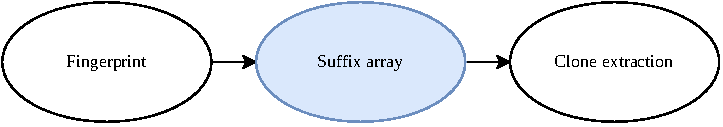
\includegraphics[width=0.8\textwidth]{figures/phases/phases_suffix.drawio.pdf}
    \end{center}
\end{figure}

With the edit operations which describes how the fingerprint has changed, the next phase
is to input the edit operations into an algorithm which dynamically updates the extended
suffix array. The algorithm discussed in this section will be run once for each edit
operation.

Constructing/updating the extended suffix array is the most time-consuming phase of the
algorithm, so the goal for the dynamic update is to take the previous suffix array and an
edit operation, and compute the new suffix array faster than building the suffix array
from scratch. We will also in a following section convert the suffix array into a dynamic
structure, which allows insertions, deletions and increments multiple elements faster than
linear time.

The algorithm used is the algorithm presented by Salson et al.~\cite{DynamicBWT,
DynamicExtendedSuffixArrays}. This algorithm is presented as two algorithms, one which
dynamically updates the BWT and one which dynamically updates an extended suffix array
based on the BWT changes. We will first discuss how the BWT is updated and how that
relates to updates in the suffix array. In the next section, we will present a new data
structure which is more efficient for representing the suffix array in a dynamic setting,
and then explain how the LCP array can be attached to this data structure. The original
paper also describes how to incrementally update the ISA, but this will be omitted, as our
new data structure contains the ISA implicitly.

Recall that the BWT is a transform on an input string which is often used for compression
and text-search purposes. The BWT is also reversible by using the LF function to compute
the original string in reverse. The LF function is computed for a position $i$ such that
$LF(i) = rank_{BWT[i]}(i) + C[BWT[i]]$ where the array $C$ contains for any character $c$,
how many characters are lexicographically smaller than $c$. This function can intuitively
be used in the context of the BWT to allow us to move from $CS_i$ to $CS_{i-1}$. Also
recall that the suffix array and the BWT of a string is highly correlated to the point
where one can compute the BWT from the suffix array in a single pass. Any updates to the
BWT will also correspond to similar updates to the suffix array, so the algorithm which
updates the BWT can be used to determine how the suffix array changes as well.

\subsection*{Updating BWT on insertion}

We will observe which parts of a BWT changes when we insert a single character. The
approach for deletions and substitutions are similar, and this approach can easily be
extended to edit operations of more than one character. Note that we are only storing the
BWT in a data structure, not the whole cyclic-shifts. We will consider an insertion of a
character $c$, inserted at position $i$. When $c$ is inserted, we know that we will have
exactly one more $CS$ for the string, which starts with the inserted character $c$, at
position $i$. This $CS$ ends with the character at position $i - 1$. We also know that
exactly one $CS$ will change its last character, which is the CS previously starting at
position $i$, but is at position $i + 1$ after the insertion. This new $CS$ will end with
the inserted character, $c$. These are the only changes that happen to the characters in
the BWT, but as we will see, the ordering of the BWT characters may not be correct
anymore.

\begin{table}[t]
	\begin{center}
		\subfloat[S = BANANA\$]{
			\begin{tabular}{c | l}
				Order & Cyclic-shift \\
				\hline
				6     & \$BANAN\textbf{A}   \\
				5     & A\$BANA\textbf{N}   \\
				3     & ANA\$BA\textbf{N}   \\
				1     & ANANA\$\textbf{B}   \\
				0     & BANANA\textbf{\$}   \\
				4     & NA\$BAN\textbf{A}   \\
				2     & NANA\$B\textbf{A}   \\
			\end{tabular}
		}
        \hspace{1cm}
		\subfloat[S = BABNANA\$]{
			\begin{tabular}{c | l}
				Order & Cyclic-shift \\
				\hline
				7     & \$BABNAN\textbf{A}   \\
				6     & A\$BABNA\textbf{N}   \\
				1     & ABNANA\$\textbf{B}   \\
				4     & ANA\$BAB\textbf{N}   \\
				0     & BABNANA\textbf{\$}   \\
				2     & BNANA\$B\textbf{A}   \\
				5     & NA\$BABN\textbf{A}   \\
				3     & NANA\$BA\textbf{B}   \\
			\end{tabular}
		}
		\caption{BWT for string before and after insert}
		\label{table:bwtupdate}
	\end{center}
\end{table}

For the string \verb|BANANA$|, let $c = \verb|B|$, and $i = 2$, which results in the
string \verb|BABNANA$|. In table \ref{table:bwtupdate} we can see that some substrings of
the BWT is preserved, such as \verb|$AA| and \verb|AN|, but some other changes have
occured. In table \ref{table:bwtupdatestages} We see that the new $CS_2$ is
\verb|BNANA$BA|, and the changed $CS_3$ is \verb|NANA$BAB|. We can find where these
cyclic-shifts are located by first looking up $i$ in the ISA, $\ISA{2} = 6$. This is the
location of $CS_3$ (after the insertion), where the final character is updated to the
inserted character \verb|B|. To find the position where the new cyclic-shift should be
inserted, we can use the LF function to move from the $CS_3$ to $CS_2$. Computing
$LF(6)$ after the substitute gives us $5$, which is where the new $CS_2$ should be
inserted in the BWT. When we insert in the BWT, we only need to consider the final
character of $CS_2$, which in this case is \verb|A|, the character which was previously
substituted.

\begin{table}[t]
	\begin{center}
		\subfloat[Original BWT]{
			\begin{tabular}{c | l | l}
				Order & F  & L           \\
				\hline
				6     & \$ & A  \\
				5     & A  & N  \\
				3     & A  & N  \\
				1     & A  & B  \\
				0     & B  & \$ \\
				4     & N  & A  \\
				2     & N  & A  \\
			\end{tabular}
		}
		\hspace{1cm}
		\subfloat[After change and insert]{
			\begin{tabular}{c | l | l l}
				Order & F  & L  \\
				\hline
                7     & \$ & A & \\
				6     & A  & N & \\
				4     & A  & N & \\
				1     & A  & B & \\
                0     & B  & \$& \\
                2     & \textbf{B}  & \textbf{A} & Inserted \\
                5     & B  & A & \\
                3     & \textbf{N}  & \textbf{B} & $A \rightarrow B$ \\
			\end{tabular}
		}
		\hspace{1cm}
		\subfloat[After reordering]{
			\begin{tabular}{c | l | l l}
                Order & F  & L & \\
				\hline
                7     & \$ & A & \\
                6     & A  & N & \\
                1     & \textbf{A}  & \textbf{B} &  \multirow{2}{*}{$\updownarrow$} \\
                4     & \textbf{A}  & \textbf{N} & \\
                0     & B  & \$& \\
                2     & B  & A & \\
                5     & B  & A & \\
                3     & N  & B & \\
			\end{tabular}
		}
		\caption{BWT for string before and after insert}
		\label{table:bwtupdatestages}
	\end{center}
\end{table}


The final stage of the algorithm now that all the elements are present, is to rearrange
the cyclic-shifts which have changed their lexicographical ordering. It is possible that
the cyclic-shifts change their ordering because of the new character. For example
\verb|ANANA$B| $<$ \verb|ANA$BAN|, but \verb|ABNANA$B| $>$ \verb|ANA$BABN|. A useful
observation is that only $CS_j$ where $j \leq i$ will have their lexicographical ordering
changed. This is because only in these cyclic-shifts the inserted character $c$ comes
before the \verb|$|. Since the \verb|$| is the smallest lexicographical character, and no
two cyclic-shifts will have \verb|$| in the same location, we know that the
lexicographical comparison of two cyclic-shifts will never go past the \verb|$|.

We know that only $CS_j$ where $j \leq i$ can have their ordering changed, and we have
already inserted $CS_i$ at the correct position (the new cyclic-shift). We will store two
positions, $pos$ and $expected$, where $pos$ is initially the position of $CS_{i - 1}$,
which was stored before any changes were made to the BWT. $pos$ is therefore the actual
position of $CS_{i - 1}$, $expected$ is the expected position of $CS_{i - 1}$, which is
computed by computing $LF(insertionPoint)$ where $insertionPoint$ is the position where
the new $CS_i$ was inserted. With the knowledge of where the cyclic-shift of order $i - 1$
is, and where we expect it to be, we can move the cyclic-shift to that position. In the
example, we have that $expected = 3$, and $pos = LF(5) = 2$ after the insertion gives us
the expected location of the cyclic-shift of order $1$. Therefore, we remove the
cyclic-shift at position $3$, and insert it again at position $2$.

Before we move the character, we also compute $newPos = LF(pos)$ which will give us the
position of the cyclic-shift of order $i - 2$. After the move, we can continue comparing
the position and expected position by updating $pos = newPos$, and $expected =
LF(expected)$. In the example this would update both $pos$ and $expected$ to $4$. Since
the expected position and actual position is the same, the algorithm is done, and we know
that every position of the BWT is now in the correct location. We know that there will be
no more characters which are out of place for any other $CS$ down to order $0$ because
$LF(pos) = LF(expected)$, which would be true for all future iterations as soon as $pos =
expected$

\subsection*{Updating SA on insertion}

The suffix array is updated similarly to the BWT. When we insert the new CS at position
$5$ in the BWT, we similarly insert the value $2$ at position $5$ in SA. We insert the
value $2$ because the new suffix which corresponds to the new cyclic-shift starts at the
position where the new character was inserted, which was $2$. When the new CS is inserted,
we are now in an invalid state for the suffix array, because we have two elements with the
value $2$. Note that a suffix array is always a permutation of the values $(0..n)$ where
$n$ is the number of characters in the input. Since we have inserted a new suffix in the
suffix array which is the 2nd smallest suffix, all the previous suffixes which had a value
$j \geq 2$ is now incremented. After incrementing all these suffixes, we are now in a
valid suffix array state, but similarly to our BWT, some suffixes may have had its
ordering changed. For every reordering operation in the BWT, the elements in SA are
reordered in the same fashion.

\begin{algorithm}[t]
  \SetAlgoLined\DontPrintSemicolon
    \algo{\UpdateSuffixArrayInsert{SA, ISA, BWT, i, ch}}{
        $\Var{posFirstModified} \gets \ISA{\Var{i}}$ \;
        $\Var{previousCS} \gets \LF{$\Var{BWT}, \Var{i}$}$ \;\;

        $\Var{storedLetter} \gets \ArrayAccess{\Var{BWT}}{\Var{posFirstModified}}$ \;
        $\ArrayAccess{\Var{BWT}}{\Var{posFirstModified}} \gets \Var{ch}$ \;\;

        $\Var{insertionPoint} \gets \LF{$\Var{BWT}, \Var{i}$}$ \;
        \lIf{$\Var{storedLetter} < \Var{ch}$} {
            $\Var{insertionPoint} \gets \Var{insertionPoint} + 1$
        } \;

        \Comment{Insert storedLetter in BWT at pointOfInsertion}
        \Insert{$\Var{BWT}, \Var{insertionPoint}, \Var{storedLetter}$}\;\;
        \Comment{Insert i in SA at pointOfInsertion, increment all values $\geq$ position}
        \Insert{$\Var{SA}, \Var{insertionPoint}, \Var{pos}$}\;
        \IncrementGreaterThan{$\Var{SA}, \Var{pos}$}\;\;


        \lIf{$\Var{insertionPoint} \leq \Var{previousCS}$} {
            $\Var{previousCS} \gets \Var{previousCS} + 1$
        } \;


        $\Var{pos} \gets \Var{previousCS}$ \;
        $\Var{expected} \gets \LF{$\Var{insertionPoint}$}$ 

        \While{$\Var{pos} \neq \Var{expected}$}{

            $\Var{newPos} \gets \LF{$\Var{pos}$}$ \;\;

            \Comment{Delete value at pos and reinsert at expected in BWT and SA}
            \MoveRow{$\Var{pos}, \Var{expected}$} \;\;

            $\Var{pos} \gets \Var{newPos}$ \;
            $\Var{expected} \gets \LF{$\Var{expected}$}$ \;

        }
    }

  \vspace{0.5cm}
  \caption{Update BWT and suffix array when inserting a single character}
  \label{alg:updatesuffixarrayinsert}
\end{algorithm}

Algorithm \ref{alg:updatesuffixarrayinsert} dynamically updates a suffix array and BWT
when a single character is inserted. This algorithm can easily be extended to insert a
string instead of a single character by adding a loop which continuously updates the
\verb|pointOfInsertion| to the previous $CS$ with the LF function, and inserts all the
characters at that position into the BWT and SA backwards. This is more efficient than
calling the single character algorithm multiple times, because the reordering stage is
only performed once. The details for insertions/deletions of multiple characters is
covered in the original paper~\cite{DynamicExtendedSuffixArrays}.

\subsection*{Deletion}

A deletion of a single character is a similar procedure as an insertion, as it is simply
reversing the substitution and insertion, and then performing the reordering stage again.
If we have the string \verb|BABNANA$|, and delete the \verb|B| at position $2$, We know
that there will be exactly one $CS$ removed. This is $CS_2$ which starts with the deleted
character \verb|B|, and ends with the character before it, \verb|A|. There is also a
single $CS$ which will have its final character changed, $CS_3$, because the final
character \verb|B| will be deleted. The final step is to again perform the reordering
stage for $CS_j$ where $j \leq 2$, as these are the only cyclic-shifts which can have
their lexicographical ordering changed.

The algorithm which performs the deletion at position $i$ will do the deletion and
substitution in the opposite order. First we find both the $CS$ which will have its
character substituted in the BWT, and the $CS$ which will have its character deleted in
the BWT. The character to be substituted will be found with $substituted = ISA[i + 1]$,
and the character to delete will be found with $deleted = LF(substituted)$. $BWT[deleted]$
is then deleted, and $BWT[substituted]$ is substituted with the character that was
deleted. Finally, the reordering phase is performed in the same fashion, where $pos$ is
set to the position of the original $CS_{i - 1}$ and $expected$ is set to $LF(substituted)$

In our example $substituted = ISA[3] = 7$, $deleted = LF(7) = 5$ and $pos = LF(5) = 2$.
Then $BWT[deleted]$ is deleted, and $BWT[substituted]$ is set to the deleted character.
Then $expected = LF(6) = 3$. Note that $substituted$ was decremented after the deletion
because the deletion moved that $CS$ one position up. When the reordering stage happens,
we have $pos = 2$ and $expected = 3$, so we perform the reordering in the BWT and SA in the
same fashion as previously, and the algorithm will again terminate after one iteration of
the reordering phase.

\subsection*{Substitution}

Substitution operations are also possible and covered in the original paper, but in
CCDetect-LSP these were simply implemented as a deletion followed by an insertion. This is
less efficient than a single operation, since the reordering stage is done twice, but we
do not suspect that this will worsen the performance in any significant way.

\subsection*{LF function}

The LF function is used multiple times for any suffix array update. Therefore, it is
important to be able to efficient compute $LF$ at any point in time. The naive approach of
linearly iterating through the BWT to compute the $rank$ and number of smaller characters
is too slow. Recall that $LF(i) = rank_{BWT[i]}(i) + C[BWT[i]]$ where $rank_{BWT[i]}(i)$
is the rank for the character $BWT[i]$ at position $i$ in the BWT, and $C[BWT[i]]$ counts
the number of lexicographically smaller characters than $BWT[i]$ in the BWT. We therefore
need a data structure for $rank$ queries on the BWT, and a data structure which stores the
number of smaller characters of each character in the BWT. 

For the $rank$ queries, recall that the wavelet matrix was a data structure which could
efficiently compute $rank/select$ queries for strings. The data structure is implemented
as a matrix of dynamic bitsets, where we also stored the number of 0 bits in each level.
Traversing this matrix from top to bottom and performing rank queries on the dynamic
bitsets in each level allows us to perform access, rank and select queries efficiently for
a string input. We will use the wavelet matrix to store the BWT and perform efficient
$access$ and $rank$ queries on it as needed. With the wavelet matrix, we do not need to
store the BWT itself, as we can simply query the wavelet matrix to access characters of
the BWT. We also do not need to store the full fingerprint, since we can access characters
in the wavelet matrix and if we need to access the characters in a sorted order, we can
use the LF function. We decided to use the wavelet matrix instead of a wavelet tree as it
has been shown to have faster $rank$ queries, and is more memory efficient for larger
alphabets. Our alphabet can be quite large compared the standard applications of
$rank/select$ data structures (such as DNA analysis). The wavelet matrix is also generally
simpler to implement, and can be dynamically updated in a simple manner. Each bitset in
the wavelet matrix is a dynamic bitset where we can efficiently insert and delete
characters as needed when the size of the BWT grows/shrinks.

When inserting a character $c$ into the wavelet matrix at position $i$, we insert the
first bit of $c$ in level $0$ in the matrix at position $i$. The next bit of $c$ is then
inserted in level $1$ in the matrix at position $rank_x(WM[0], i)$ where $x$ is the value
of the previous bit. We continue this process, updating the position by performing a rank
query, and then inserting the bit at that position, until we reach the bottom of the
matrix. Similarly, for a deletion, we find each bit which was inserted for that position
in each level, and remove them. Algorithm \ref{alg:waveletmatrixinsert} shows how an
element can be dynamically inserted into the wavelet matrix. Algorithms for deletions and
substitutions are left out, but follow the same idea. Substitutions are simply implemented
as a deletion followed by an insertion.

A complication with the wavelet data structures is to update the data structure as the
alphabet increases in size. In our case the alphabet size will at some point increase to a
size where elements need an additional bit. For the wavelet matrix, this can be solved by
simply inserting a new row at the beginning of the matrix (level $0$), where the bitset
consists of all zeroes. Afterwards, the new element is inserted in the normal fashion.

\begin{algorithm}[t]
  \SetAlgoLined\DontPrintSemicolon
    \algo{\WaveletMatrixInsert{wm, index, value}}{
        $\Var{numBits} \gets \textrm{Number of bits in value}$ \;\;

        \While{$\Var{numBits} > \Len{$\Access{\Var{wm}}{\Var{levels}}$}$}{
            \textrm{Insert new row at level 0 in wm}
        } \;

        $\Var{level} \gets 0$ \;
        $\Var{currIndex} \gets \Var{index}$ \;\;

        \While{$\Var{level} < \Len{$\Access{\Var{wm}}{\Var{levels}}$}$}{
            $\Var{currentBit} \gets
            \Len{$\ArrayAccess{\Access{\Var{wm}}{\Var{levels}}}{\Var{level}}$} -
            \Var{level} - 1$ \;\;

            \Comment{Get the bit value at position currentBit in value}
            $\Var{bit} \gets \GetBit{$\Var{value}, \Var{currentBit}$}$ \;\;

            \Comment{Insert the bit into the bitset at position currIndex}
            \Insert{$\Access{\Var{wm}}{\Var{level}}, \Var{currIndex}, \Var{bit}$} \;\;


            \Comment{Update currIndex to the position to insert in the next level}
            $\Var{currIndex} \gets \RankBit{$\Access{\Var{wm}}{\Var{level}}, \Var{currIndex}$}$ \;\;

            \Comment{If the bit we inserted is 1, add the number of zeroes in the level}
            \If{$\Var{bit} = 1$}{
                $\Var{currIndex} \gets \Var{currIndex} + \Access{\Access{\Var{wm}}{\Var{level}}}{z_l}$
            }
            $\Var{level} \gets \Var{level} + 1$


        }
    }

  \vspace{0.5cm}
  \caption{Dynamically insert an element into the wavelet matrix}
  \label{alg:waveletmatrixinsert}
\end{algorithm}

The $C$ array can be implemented in two ways. Either $C[c]$ holds the number of smaller
character than $c$ in the input, or $C[c]$ holds the number of occurrences of $c$. There
are trade-offs with either implementation, as storing the number of smaller characters
requires a linear scan whenever a character is inserted or deleted, while storing the number
of occurrences requires a linear scan to compute the number of smaller characters whenever
the LF function is called. We have chosen the approach of storing the number of
occurrences, as updating the array is simpler in cases where the alphabet size increases.
When we later update LCP values, we will see that there is a possibility that choosing the
option of storing the number of smaller characters in $C$ is faster. 

\section{Dynamic extended suffix arrays}

A major bottleneck when inserting or deleting elements in the suffix array is that when an
element is for example removed, all elements after it needs to be moved by one index so
that the gap is closed. This is also the case in the reordering stage, where all the
elements between the old position and new position of an element needs to be moved by one
position. In addition, since a suffix array is always a permutation from $0$ to $n - 1$
where $n$ is the number of elements in the input, we need increment/decrement all elements
greater than or equal to the element which was inserted or deleted. For example, if we
insert a new element into the suffix array which indicates that a new suffix is the ith
smallest, then the previous suffix with value $i$ in SA should now have the value $i + 1$,
which applies to all other suffixes lexicographically greater than the new suffix as well.
In a standard representation for a suffix array (an array), this would require either a
linear scan through the entire SA, or a linear scan through ISA from position $i$, which
is also linear in the worst case. Multiple linear scans through the SA would make the
algorithm slower than the linear time SACA when the amount of inserted or deleted
character increases. 

In this section we will introduce a data structure we call the dynamic extended suffix
array. This data structure consists of a dynamic permutation, which facilitates insertion
and deletion of elements in a permutation from $0$ to $n - 1$, without linear scans to
close gaps or incrementing/decrementing elements. The data structure stores SA, ISA and
LCP and is inspired by the data structure introduced for the same purpose by Salson et
al.~\cite{DynamicExtendedSuffixArrays}. The data structure used by Salson et al. uses the
same dynamic permutation tree, but reduces the amount of values which is stored to reduce
memory consumption, but this compression also slows down the access time of elements in
the permutation. Our data structure will not be compressed, which allows faster access to
arbitrary elements, and will be extended to also include the LCP values as well.
Therefore, this data structure encompasses the entire extended suffix array.

The data structure consists of two balanced binary trees, with pointers between elements
in one tree to the other. Figure \ref{fig:dynamicpermutation} shows the two trees which
are labeled the $A$ tree and the $B$ tree. We will see that these trees can intuitively be
understood as a tree containing the indexes (A), and a tree containing the values (B) of
our permutation. Note that the trees do not actually hold the values displayed in the
figure, the values in each node of the figure only represents the inorder position of each
node, which is called the inorder rank of the node.

To construct a permutation of length $n$ such as $[6,5,3,1,0,4,2]$, we can insert a node
in each tree for each element. After the trees both contain $n$ nodes, pointers are added
from a node in $A$ to a node in $B$ and vice versa (doubly linked). If an element in SA
has a value $i$ at position $j$, pointers will be added between the node in $A$ with
inorder rank $i$, and the node in $B$ with inorder rank $j$. 

Now the tree is complete, but we can also insert new nodes into the data structure as the
suffix array grows. When a new value $j$ is added at position $i$, a node is inserted into
$A$ such that it has the inorder rank of $i$, and a node is inserted into $B$ such that it
has the inorder rank of $j$. For example, if we wanted to insert a new value $4$ at
position $1$ in the permutation in figure \ref{fig:dynamicpermutation}, we would insert a
new node in $A$ so that it is the right child of the node labeled $0$, and then insert a
new node in $B$ which is the left child of the node labeled $4$. The trees can intuitively
be understood such that the inorder values in $A$ represent the indices of the
permutation, and the inorder values in $B$ represent the values in the permutation.
Therefore, if we look at a node in $A$ with inorder rank $i$, and follow the pointer to a
node in $B$ with inorder rank $j$, this means that the permutation has the value $j$ at
position $i$. 

Deleting a node at position $i$ is similar, but we will instead find the node with a rank
of $i$ in $A$, then delete that node and the node it points to in $B$. As the trees are
implemented as balanced trees, traversing, inserting and deleting nodes takes $O(\log n)$
time.

An essential property of this tree is that when a new value $j$ is inserted into the
permutation at position $i$, all indices $\geq i$ and values $\geq j$ is incremented by
$1$. This is because all the nodes which had an inorder rank greater than or equal to the
new nodes in each respective tree has now been incremented by $1$ simply because the
structure of the tree has changed. No additional work is required to increment the
elements. 

The part we are still missing is how to find a node with inorder value $i$, and how to
determine the inorder value of a given node. We cannot afford to traverse all the nodes in
an inorder fashion to find a node with a specific inorder rank. Therefore, the trees are
implemented as order-statistic trees~\cite[340]{CLRS}. An order-statistic tree is a tree
where each node $x$ stores an additional integer $size$, which contains the number of
nodes in the subtree rooted at $x$. This allows us to easily determine how many nodes is
in the left subtree of a given node, and use this to determine where the node with a
certain inorder rank is located. If we wanted to find the node in the $A$ tree of figure
\ref{fig:dynamicpermutation} with inorder rank $4$, we would start at the root, see that
the left subtree of the root contains $3$ nodes. Therefore, the roots inorder rank is $3$.
With this information we know that we need to traverse to the right child, and look for
the node with inorder rank $4 - 4 = 0$ in that subtree (since we have already seen 4
nodes). Since the node labelled $5$ has a rank of $1$ (in its own subtree), we know to
traverse left, and at that point we have reached the correct node.

\begin{figure}[t]
	\begin{center}
		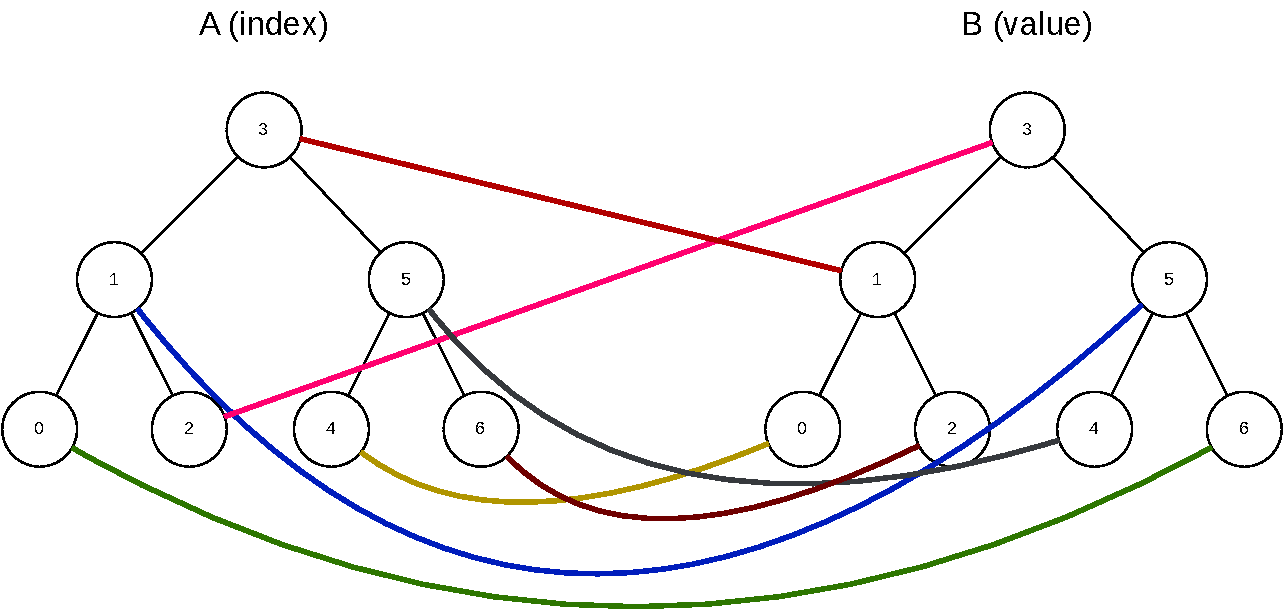
\includegraphics[width=0.95\textwidth]{figures/dynamicpermutation.drawio.pdf}
	\end{center}
	\caption{Dynamic permutation for the permutation $[6,5,3,1,0,4,2]$. Colors have no meaning except to make lines clearer}
	\label{fig:dynamicpermutation}
\end{figure}

\begin{algorithm}[t]
  \SetAlgoLined\DontPrintSemicolon
    \algo{\GetNodeByRank{root, rank}}{
        $\Var{current} \gets \Var{root}$ \;

        \While{$\Var{current} \neq \Null$}{
            $\Var{currentRank} \gets \Access{\Access{\Var{current}}{\Var{left}}}{\Var{size}}$

            \uIf{$\Var{currentRank} = \Var{rank}$}{
                \Break \;
            }
            \uElseIf{$\Var{currentRank} > \Var{rank}$}{
                $\Var{current} \gets \Access{\Var{current}}{\Var{left}}$
            }
            \Else{
                $\Var{current} \gets \Access{\Var{current}}{\Var{right}}$ \;
                $\Var{rank} \gets \Var{rank} - \Var{currentRank} + 1$
            }
        }
        \Return $\Var{current}$
    }

  \vspace{0.5cm}
  \caption{Find the node in a tree with a given inorder rank}
  \label{alg:getnodebyrank}
\end{algorithm}

\begin{algorithm}[t]
  \SetAlgoLined\DontPrintSemicolon
    \algo{\GetRankOfNode{node}}{
        $\Var{rank} \gets \Access{\Access{\Var{node}}{\Var{left}}}{\Var{size}}$ \;
        \While{$\Access{\Var{node}}{\Var{parent}} \neq \Null$}{
            \If{$\Access{\Access{\Var{node}}{\Var{parent}}}{\Var{right}} = \Var{node}$}{
                $\Var{rank} \gets \Var{rank} + \Access{\Access{\Var{node}}{\Var{parent}}}{\Var{right}} + 1$
            }
            $\Var{node} \gets \Access{\Var{node}}{\Var{parent}}$
        }

        \Return $\Var{rank}$
    }

  \vspace{0.5cm}
  \caption{Find the inorder rank of a given node}
  \label{alg:getrankofnode}
\end{algorithm}

Algorithm \ref{alg:getnodebyrank} shows how to find a node in a tree by its inorder rank,
and algorithm \ref{alg:getrankofnode} shows how to determine the rank of a given node. The
algorithm to find the value at a certain position is simple with these algorithms. To find
the value in the permutation at position $i$, find the node with inorder rank $i$ in $A$,
follow its pointer to a node in $B$, and then find the inorder rank of that node, which is
the value at position $i$ in the permutation. We can also find the position of any value
$j$ in the permutation by performing this algorithm in reverse, by instead starting at the
$B$ tree, finding a node with rank $j$, then following its pointer to a node in $A$ and
returning that nodes inorder rank.

\begin{algorithm}[t]
  \SetAlgoLined\DontPrintSemicolon
    \algo{\DynamicPermutationAccess{permutation, i}}{
        $\Var{aNode} =
        \GetNodeByRank{$\Access{\Access{\Var{permutation}}{\Var{A}}}{\Var{root}}, \Var{i}$}$ \;
        $\Var{bNode} = \Access{\Var{aNode}}{\Var{pointer}}$

        \Return \GetRankOfNode{$\Var{bNode}$}
    }

  \vspace{0.5cm}
  \caption{Get value at position $i$ in a permutation}
  \label{alg:dynamicpermutationaccess}
\end{algorithm}

With the ability to both find a value at a given position in the permutation, and also
finding the position of a given value, we can use this data structure to represent the
suffix array and inverse suffix array, instead of a simple array. Inserting, deleting and
accessing a node in this data structure takes $O(\log n)$ time, and we no longer need a
linear scan through the data structure to increment/decrement values, as values are
automatically incremented/decremented when a new element is inserted or deleted.

\section{Dynamic LCP array updates}

Now that we have a dynamic structure to represent SA and ISA, we can extend the data
structure to also contain the LCP array, and efficiently update the LCP values as well.

Since every node in the $A$ tree of our data structure correlates to an index, we can
easily extend the data structure to contain LCP values by setting a value in each node of
the $A$ tree. This would make the $A$ tree work as a balanced binary tree for the LCP
values, and if an SA value at position $i$ is deleted, the LCP value stored in
the respective node is also deleted.

In the initial construction of the dynamic permutation, LCP values would be inserted
together with the nodes. When dynamically updating the LCP values as suffixes are
inserted/removed, the procedure is more complicated. Salson et
al.\cite{DynamicExtendedSuffixArrays} also describe a procedure for updating the LCP
values after an insert/delete operation, which we will use.

When inserting a character into the input string, the suffix array changes by inserting a
new value, and afterwards moving values from one position to another (reordering stage).
Similarly, a deletion in the suffix array consists of deleting a value, and performing the
same reordering operations. The moving of a value from position $i$ to $j$ can be
decomposed into a deletion at position $i$ followed by an insertion at position $j$. When
updating the LCP array we therefore need to consider how insertion of a value and deletion
of a value in SA affects the LCP values.

The idea for this algorithm is to keep track of all positions which could have its LCP
value changed, and update the LCP values after the SA is fully updated. There are four
different cases where an LCP value at a position $i$ could be changed:

\begin{enumerate}
    \item A suffix was inserted at position $i - 1$ in SA, which is the new suffix that
        the suffix at position $i$ should compute its LCP value for.

    \item The suffix at position $i - 1$ was deleted in SA, making the suffix at position
        $i - 2$ the new suffix that the suffix at position $i$ should compute its LCP
        value for.

    \item A character was inserted or deleted in the middle of the LCP for the suffix at
        position $i$ in SA, which shortens the LCP value between it and the suffix at
        position $i - 1$, and the LCP value between the suffix at position $i$ and $i + 1$.

    \item A character was inserted or deleted at the end of the LCP for the suffix at
        position $i$ in SA, which could potentially extend the LCP value between it and
        the suffix at position $i - 1$, and the LCP value between the suffix at position
        $i$ and $i + 1$.

\end{enumerate}

To cover the first two cases, we will store a dynamic bitset where a set bit at position
$i$ indicates that at some point, the LCP value at position $i$ needs to be updated.

For an insertion at position $i - 1$ in SA (case 1), we will set the bit at position $i$,
as the suffix it compares its LCP to has changed. We will also insert a set bit at
position $i - 1$, as the newly inserted suffix also needs to compute its LCP value with
the suffix at position $i - 2$.

Similarly, for a deletion at position $i - 1$ in SA (case 2), we will set the bit at
position $i$, as the suffix it used to compare its LCP to has been deleted. We will also
delete the bit at position $i - 1$, as the suffix at that position has been deleted.

After setting these bits while performing an insert/delete operation in the SA, the bitset
now contains all the positions of LCP values which need to be updated for the first two
cases. The other two cases are more complex to find the positions of. Instead of inserting
the positions of these suffix into the bitset, we will iterate over the suffixes which
could possibly have their LCP value changed. Iteration over every suffix and recomputing
the LCP value takes linear time in the size of the fingerprint and is therefore too slow
for this algorithm. However, we can reduce the number of suffixes we need to update by
applying a series of observations.

The first observation is that we only need to consider suffixes where the
insertion/deletion of a character at position $i$ has changed the suffix. Those are the
suffixes which start at a position $j$ where $j \leq i$. Other suffixes cannot change, as
the insertion/deletion happened before the starting position of the suffix. For a suffix
at position $j$ which has changed, two LCP values can change, the values at position $k$
and $k + 1$ where $SA[k] = j$. These two LCP values can change, because at position $k$,
the suffix at position $SA[k]$ is compared with $SA[k - 1]$, and at position $k + 1$, the
suffix at position $SA[k + 1]$ is compared with $SA[k]$. Since both of these LCP values
depend on the suffix at position $SA[k] = j$, they can potentially change when the suffix
is changed. The positions in SA which possibly can be changed can be found using the LF
function. In the final phase of the suffix array update algorithm when we have inserted or
deleted an element at position $i$, we are reordering suffixes at position $j \leq i$.
These are the suffixes we are looking for, but we can skip all suffixes which are
reordered, as they are already marked to be computed in the bitset for the previous cases.
Therefore, the variable $pos$ points to the next suffix we need to consider at the end of
algorithm \ref{alg:updatesuffixarrayinsert}.

Another useful observation when iterating over suffixes is that after an
insertion/deletion, no two suffixes will have the insertion/deletion occur at the same
position. This is true because no two suffixes start on the same position in the input,
and an insertion/deletion at a position $i$ in the input can therefore never correspond to
an insert/deletion at the same position for two different suffixes. With that in mind,
another useful observation is that given two suffixes with an LCP value of $p$, any change
inside the range of the LCP in either of the suffixes, will change $p$.

The idea is to determine if the insertion/deletion is out of range to possibly affect the
LCP value of a suffix. Recall that the LCP value for a suffix at position $i - 1$ is at
minimum one less than the LCP value for the previous suffix at position $i$, as discussed
in \cref{initialdetection}. We can determine that it is impossible for the LCP value at
position $i - 1$ to change, if neither of the LCP values which is affected by the suffix
at position $i$ changes, unless the insertion/deletion happens at position $i - 1$. This
is explained by the fact that at minimum, the LCP of the suffix at position $i$ covers
every character of the LCP of the suffix at position $i - 1$ except for the first
character. If the first character was the position of the insertion/deletion, it can
change the LCP value, but that case is already handled by the positions stored in the
bitset. Since the suffix at position $i - 1$ did not update, this holds recursively for
the next suffix at position $i - 2$ as well. Therefore, as soon as we find a single suffix
at position $i$ which does not lead to an LCP value update, this will recursively hold for
all suffixes at position $j < i$.

With this in mind, the algorithm to update the LCP array has two stages. Given the bitset
of positions which need to be updated in correlation with the first two cases, we perform
a $select$ operation to continuously find the location of set bits in the bitset, and use
their position to determine which positions in the LCP array need to be computed. After
all the positions in the bitset has been updated in the LCP array, we move on the last two
cases. From the position of $pos$, which was computed during the suffix array update, we
continuously call the LF function on $pos$ to find the previous suffix. At each position,
we update the LCP value of the suffix at position $pos$ and $pos + 1$, as these two LCP
values are both affected by the suffix at position $SA[pos]$. When we encounter the
situation where both LCP values at position $pos$ and $pos + 1$ did not lead to a change
in LCP values, the algorithm is finished and the LCP array is updated. Algorithm \ref{}
shows how the LCP array is updated, given the bitset of updated positions which is built
during algorithm \ref{alg:updatesuffixarrayinsert}.

The actual computation of LCP values is also fairly complex. In the incremental detection
algorithm we are not storing the entire fingerprint, we only have the BWT stored in the
wavelet matrix, and the LF function allows us to move from one character to the previous
in the original input text. When we compute LCP values, we need to be able to compare
characters in two suffixes from start to potentially end of the input, therefore we need
to be able to move from one character to the next, which is the inverse of the LF
function. 

The inverse LF function for a position $i$ computes the next cyclic-shift by first
determining what character is in the first column of the CS at position $i$ in the sorted
cyclic-shifts, and its $rank$ in the first column. With the character and rank of that
character, we can perform a $select$ on the BWT for that character and rank, which will
give us the location of where that character is located in the last column (BWT) which is
the next CS. This is the next cyclic-shift because it is the cyclic-shift where the
character which was previously in the first column, but is now cycled one character to the
left, which corresponds to the next CS. To find which character is in the first column at
position $i$, recall that the $F$ column in the sorted cyclic-shifts just contain all the
characters of the input in sorted order. We can therefore use the $C$ to determine which
character is located at exactly position $i$, just by counting the number of occurrences
of the previous characters. If $C$ is instead implemented as an array where the $C[c]$
holds the number of characters smaller than $c$ in the input, finding the correct
character can be done efficiently with a binary search. When we know which character is
located at position $i$ in the first column, we do $select_c(i - C[c])$ to determine where
that occurence of $c$ is located in the last column (the BWT), which is then returned as
the result of the inverse LF function.

With the inverse LF function, computing the LCP value between two suffixes at position $i$
and $j$ is done by repeatedly applying the inverse LF function to $i$ and $j$, and
comparing the characters at those positions in the BWT.

\Todo{Algorithm for iterating over suffixes which need to update their LCP value}

\Todo{Algorithm for updating a single LCP value}

\Todo{Visualize this somehow?}

\section{Dynamic clone extraction and source-mapping}

\begin{figure}[H]
    \begin{center}
        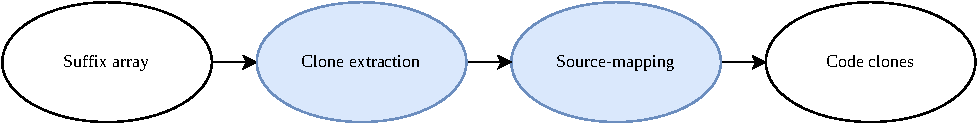
\includegraphics[width=1\textwidth]{figures/phases/phases_extractionandsourcemap.drawio.pdf}
    \end{center}
\end{figure}

The LCP array is no longer implemented as an array, but as a balanced tree. As trees are
more costly to traverse linearly compared to arrays, we also want to improve how we
extract clones in this phase. The goal of the clone extraction phase is still to find the
indices in the fingerprint which corresponds to the beginning of a code clone in the
original source code. These indices will be mapped back to the original source code in the
source-mapping phase.

Recall that the initial detection clone extraction algorithm in \cref{initialdetection}
traversed the suffixes from beginning to end, and extracts indices of suffixes where the
LCP value is above the token threshold parameter. Also recall that some clones were
filtered, those being clones which extend past a single fragment, or clones which are
contained inside a larger clone. This algorithm will now be converted to run on the
balanced tree which contains the LCP values, which also optimizes the algorithm to reduce
the amount of LCP values we need to examine.

The idea for this algorithm is to always store a list of all the nodes in the tree which
have an LCP value above the token threshold. These are afterall the only nodes which could
possibly be the beginning of a code clone, even if some of them will be filtered out
later. When a value is updated, we can check to see if the new value is above the token
threshold. If the previous value was below the threshold, and the new value is above the
threshold, we know that this is a node which could potentially be a code clone, so storing
these nodes can reduce the amount of nodes we need to examine. When all LCP values have
been updated, we can filter out nodes which have had their LCP value updated to be below
the threshold.

After all LCP values are updated, we are left with a set of all the nodes with an LCP
value above the token threshold. In order to filter out clones which are contained within
other clones, we need to add a similar check to the loop which was added in Algorithm
\ref{alg:cloneextraction}, however since the set only contains nodes with LCP values above
the token threshold, the algorithm will be slightly different. Instead of adding a loop
which skips past indices which are contained clones, we can instead check if the last node
which was deemed the start of a code clone contains the current clone we are looking at.
Doing the process in this fashion allows us to skip checking many nodes if there are long
stretches of suffixes in the fingerprint with LCP values below the token threshold.
Algorithm \ref{alg:dynamiccloneextraction} shows how these clone indices are computed.

\begin{algorithm}[t]
  \SetAlgoLined\DontPrintSemicolon
    \algo{\DynamicCloneExtraction{nodesAboveTreshold}}{
        $\Var{clones} \gets \textrm{empty\ list}$

        $\Var{lastAdded} \gets -1$ \;
        $\Var{lastLCP} \gets -1$ \;

        \For{$\Var{node} \In \Var{nodesAboveTreshold}$}{
            
            $\Var{index} \gets \GetRankOfNode{$\Access{\Var{node}}{\Var{pointer}}$}$ \;

            \If{$\Var{lastAdded} \neq -1$}{
                $\Var{difference} \gets \Var{index} - \Var{lastAdded}$ \;
                \If{$\Access{\Var{node}}{\Var{key}} + \Var{difference} \leq \Var{lastLCP}$}{
                    \Continue
                }
            }

            \Add{$\Var{clones}, \Var{node}$} \;
            $\Var{lastAdded} \gets \Var{index}$ \;
            $\Var{lastLCP} \gets \Access{\Var{node}}{\Var{key}}$
        }

        \Return $\Var{clones}$
    }

  \vspace{0.5cm}
  \caption{Extract clone indices in dynamic extended suffix array}
  \label{alg:dynamiccloneextraction}
\end{algorithm}

After applying this algorithm we are left with the nodes with inorder ranks which
correspond to the same indices as in the initial detection For the final phase, which
involves mapping the clone indices back to the original source code, we can do almost the
same procedure as in the initial detection. This algorithm is almost the same as algorithm
\ref{alg:buildclonemap}, but some parts are changed to avoid traversing through the trees
many times to find the second index, which we would have to do if we used algorithm
\ref{alg:buildclonemap} without any modifications. The problem with algorithm
\ref{alg:buildclonemap} is that it computes the expression $\SA{\ISA{\Var{firstIndex}} -
1}$ to find the index of the matching clone. This is not a problem in the initial
detection, because SA and ISA are arrays, which give $O(1)$ time access. This is not the
case for the dynamic extended suffix array, which would require $O(\log n)$ access time
for that expression. Instead, only the nodes of the clone indices in algorithm
\ref{alg:dynamiccloneextraction} is stored, and for a node $firstNode$, when we can find
the node of the matching $secondNode$ in $O(1)$ time by finding the predecessor of
$\Var{firstNode}$ and following its pointer. Remember that the nodes we have stored as
clone indices are nodes in the $A$ tree which corresponds to $SA$ indices. Following the
pointer corresponds to SA values, or alternatively, ISA indices. After we have both the
$\Var{firstNode}$ and $\Var{secondNode}$, we can get their fingerprint indices by getting
the inorder rank of their pointer, with Algorithm \ref{alg:getrankofnode}. Afterwards, the
algorithm continues as previously. While this still requires traversing the tree in
$O(\log n)$ time, we have reduced the number of traversals needed from $5$ with a direct
translation of Algorithm \ref{alg:buildclonemap} to $2$ with the smarter traversal of
nodes described here.

Now that we have successfully source-mapped from our dynamic extended suffix arrays to
code clones, we are finished, and we have the set of clones ready to be sent to the
client.


\chapter{Evaluation}


We will evaluate this tool based on different criteria, which combined will provide a
basis for evaluating the tool as a whole.

Since the tool is focused on efficient detection and management of code clones, real-time
performance of the tool will be a high priority in its evaluation. The tool will implement
different techniques of detecting and merging clones. These will be empirically compared
against each other. The tool will also be evaluated against existing tools empirically. We
will utilize BigCloneBench~\cite{BigCloneBench} to evaluate detection techniques, by
running our detection techniques in a standalone mode. We will distinguish between initial
detection and incremental detection when evaluating.

The tool will also be evaluated in how well it fits into the software development cycle.
Can we determine if this tool is an effective way to detect a clone early in its lifecycle
so that they can be removed before it manifests in the source code? In relation to this,
we will evaluate if LSP is a suitable tool for use in clone management and refactoring in
general. Can LSP provide all the features one would want in a modern analysis tool? What
is missing, and how could the LSP protocol be extended in order to facilitate this? We
believe that if LSP is an appropriate tool to use for clone management, LSP will also be
an appropriate tool for static analysis tools in general.


\chapter{Discussion}

\section{Performance}

\section{Clones}

\chapter{Conclusion and future work}

The results show that CCDetect incremental algorithm outperforms the other two algorithms
both in terms of time and memory on larger code bases. Our algorithm was able to handle
large edits in an IDE environment for 5.8MLOC in under 2 second,

\section{Future work}

In this section we list future work and research in order of what we consider
most interesting to do more research on, to least.

\subsection*{Type-2 and type-3 clones}

\subsection*{Optimal edit operations}

\subsection*{Refactoring of clones}

\subsection*{Compressing data structures}

\subsection*{Lazy LCP array updates}

\section{Related work}


\section{Conclusion}

\chapter{Appendix}

The appendix contains supplementary figures, logs and algorithms which do not naturally
fit into the thesis. Algorithms in this chapter are generally very verbose, and it is
recommended to read them alongside their respective explanations in the implementation
chapters.

\begin{algorithm}[htp]
  \SetAlgoLined\DontPrintSemicolon
  \algo{\WagnerFischerOperations{$S_1$, $S_2$, $\Var{matrix}$}}{
      $\Var{operations} \gets \textrm{Empty list}$\;
      $\Var{currentOperation} \gets \textrm{None operation}$ \;
      $\Var{lastOperationIndex} \gets -1$ \;
      $\Var{x} \gets \Len(\Var{matrix}) - 1$ \;
      $\Var{y} \gets \Len(\ArrayAccess{\Var{matrix}}{\Var{x}}) - 1$ \;\;

    \While{$\Var{x} > 0 \And \Var{y} > 0$}{
          $\Var{subValue} \gets \MatrixAccess{\Var{matrix}}{\Var{x} - 1}{\Var{y} - 1}$ \;
          $\Var{delValue} \gets \MatrixAccess{\Var{matrix}}{\Var{x} - 1}{\Var{y}}$ \;
          $\Var{insValue} \gets \MatrixAccess{\Var{matrix}}{\Var{x}}{\Var{y - 1}}$ \;

          \If{$\Var{subValue} \leq \Var{delValue} \And \Var{subValue} \leq \Var{insValue} \And $}{
              \If{$\Var{subValue} \neq \MatrixAccess{\Var{matrix}}{\Var{x}}{\Var{y}}$}{

                \If{$\mathrm{currentOperation\ is\ not\ a\ substitute} \Or \Var{lastOperationIndex} \neq \Var{x}$}{
                    $\Var{currentOperation} \gets \textrm{New\ substitute\ operation with
                    position } \Var{x} - 1$ \;
                    $\Insert{$\Var{operations}, 0, \Var{currentOperation}$}$ \Comment{Add operation at index 0}
                }
                \Else {
                    $\Access{\Var{currentOperation}}{\Var{position}} \gets \Access{\Var{currentOperation}}{\Var{position}} - 1$ \;
                }
              }
              Add $\ArrayAccess{\Var{S_2}}{\Var{y} - 1}$ to beginning of $\Access{\Var{currentOperation}}{\Var{chars}}$ \;
              $\Var{lastOperationIndex} \gets \Var{x} - 1$ \;
              $\Var{x} \gets \Var{x} - 1$ \;
              $\Var{y} \gets \Var{y} - 1$ \;
          }
          \ElseIf{$\Var{insValue} \leq \Var{delValue}$}{

                \If{$\mathrm{currentOperation\ is\ not\ an\ insert} \Or \Var{lastOperationIndex} \neq \Var{x}$}{
                    $\Var{currentOperation} \gets \textrm{New\ delete\ operation with position } \Var{y} - 1$ \;
                    $\Insert{$\Var{operations}, 0, \Var{currentOperation}$}$ \Comment{Add operation at index 0}
                }
                
              Add $\ArrayAccess{\Var{S_1}}{\Var{x} - 1}$ to beginning of $\Access{\Var{currentOperation}}{\Var{chars}}$ \;
              $\Var{lastOperationIndex} \gets \Var{x - 1}$ \;
              $\Var{y} \gets \Var{y} - 1$ \;
          }
          \Else{

                \If{$\mathrm{currentOperation\ is\ not\ a\ delete} \Or \Var{lastOperationIndex} \neq \Var{x}$}{
                    $\Var{currentOperation} \gets \textrm{New\ insert\ operation with position } \Var{x} - 1$ \;
                    $\Insert{$\Var{operations}, 0, \Var{currentOperation}$}$ \Comment{Add operation at index 0}
                }
                
              Add $\ArrayAccess{\Var{S_1}}{\Var{x} - 1}$ to beginning of $\Access{\Var{currentOperation}}{\Var{chars}}$ \;
                $\Var{lastOperationIndex} \gets \Var{x} - 1$ \;
              $\Var{x} \gets \Var{x} - 1$ \;
          }

      }
      \Return $\Var{operations}$
    }

  \vspace{0.5cm}
  \caption{Compute aggregated edit operations from Wagner-Fischer matrix}
  \label{alg:wagnerfischeroperations}
\end{algorithm}

\begin{algorithm}[htp]
  \SetAlgoLined\DontPrintSemicolon
    \algo{\WagnerFischerEditDistance{$S_1$, $S_2$}}{
        $\Var{n} \gets \Len{$\Var{S}_1$}$ \;
        $\Var{m} \gets \Len{$\Var{S}_2$}$ \;
        $\Var{matrix} \gets \mathrm{new\ array}[\Var{n} + 1][\Var{m} + 1]$ \;\;


        \For{$i \From 0 \To n$}{
            $\MatrixAccess{\Var{matrix}}{\Var{i}}{0} = \Var{i}$
        } \;

        \For{$i \From 0 \To m$}{
            $\MatrixAccess{\Var{matrix}}{\Var{0}}{i} = \Var{i}$
        } \;

        \For{$i \From 1 \To n$}{
            \For{$j \From 1 \To m$}{
                \If{$\ArrayAccess{\Var{S}_1}{\Var{i} - 1} = \ArrayAccess{\Var{S}_2}{\Var{j} - 1}$}{
                    $\MatrixAccess{\Var{matrix}}{\Var{i}}{\Var{j}}  = \MatrixAccess{\Var{matrix}}{\Var{i - 1}}{\Var{j - 1}} $
                }
                \Else {
                    $\Var{delete} \gets \MatrixAccess{\Var{matrix}}{\Var{i} - 1}{\Var{j}}$ \;

                    $\Var{insert} \gets \MatrixAccess{\Var{matrix}}{\Var{i}}{\Var{j - 1}}$ \;

                    $\Var{substitute} \gets \MatrixAccess{\Var{matrix}}{\Var{i - 1}}{\Var{j - 1}}$ \;\;

                    $\MatrixAccess{\Var{matrix}}{\Var{i}}{\Var{j}}  = \Min{$\Var{insert},
                    \Var{delete}, \Var{substitute}$} + 1$

                }
            }
        }

        \Return $\Var{matrix}$
    }

  \vspace{0.5cm}
  \caption{Fill edit distance matrix using Wagner-Fischer algorithm}
  \label{alg:wagnerfischerfill}
\end{algorithm}

\begin{figure}
    \begin{alltt}
        \input{logs/ccdetect.report}
    \end{alltt}
    \caption{BigCloneEval evaluation report on CCDetect-LSP}
    \label{bcblog}
\end{figure}


\printbibliography
\end{document}
